% !TEX root = ThesisGchatzi.tex

\graphicspath{{Papers/SIGSpatial2017/}{Papers/SIGSpatial2018/}}

\section{Experimental Evaluation} 
\label{sec:exp_btsr}

This chapter experimentally evaluates all our hybrid queries processing approaches and discusses the obtained results. First, we evaluate the \tsr and \btsr indices in terms of construction time and index size, in contrast with the standard R-tree. Then we evaluate the performance of \tsr and \btsr against a standard R-tree implementation, where we first apply spatial filtering and then scan through all the obtained geolocated time series to keep only the ones that satisfy $\epsilon_{ts}$. Next, we evaluate our hybrid similarity join approach using $i$SAX, R-tree and \btsr. Finally, we compare our distributed similarity join algorithm against a basic version that utilizes standard R-trees for local indexing. We first describe our experimental setup, the datasets and the applied parameterizations.

\subsection{Experimental Setup}
\label{subsec:evaluation_setup}

\begin{table}[!ht]
	\centering
	\caption{Datasets and default thresholds used in the similarity search experiments.}
	\centering
	\resizebox{\linewidth}{!}{
	\begin{tabular}{lcccccc}
	\hline
	\multirow{2}{*}{Dataset} & Area & Number of & Length of & \multicolumn{3}{c}{Default query thresholds} \\
	 & (km$^2$) & locations & timeseries & $\theta_{sp}$ & $\theta_{ts}$ & $\theta_h$ \\
	\hline
	Water & 114 & 200,000 & 168 &  0.15 & 0.175 & 0.15  \\
	Taxi & 2,500 & 417,960 & 168 & 0.2 & 0.001 & 0.0025 \\
	Flickr & Earth & 414,967 & 96 & 0.25 & 0.0005 & 0.001 \\
    Crime & 392,000 & 362,215 & 76 & 0.3 & 0.01 & 0.02 \\
	\hline
	\end{tabular}}
	\label{tab:datasets_btsr}
\end{table}

\subsubsection{Datasets}

We use four real-world datasets, which are selected from various application domains and have different characteristics, in order to evaluate our approach with diverse types of geolocated time series. Next, we describe the characteristics of each dataset. A summary is listed in Table \ref{tab:datasets_btsr}.

\emph{DAIAD Water Consumption (Water)}. Courtesy of the DAIAD project (\url{http://daiad.eu/}), we acquired a geolocated time series dataset of hourly water consumption for 822 households in Alicante, Spain from 1/1/2015 to 20/1/2017. In order to get a more representative dataset for our tests, we first calculated the weekly  ($24 \times 7$) time series per household by averaging corresponding hourly values over the entire period. Then, these weekly time series were used as seeds in order to synthetically increase the size of the dataset to 200,000, by introducing some random variations in their location and pattern.

\emph{NYC taxi drop-offs (Taxi)}. This dataset contains time series extracted from yellow taxi rides in New York City during 2015. The original data\footnote{\url{http://www.nyc.gov/html/tlc/html/about/trip_record_data.shtml}} provide pick-up and drop-off locations, as well as corresponding timestamps for each ride. For each month, we generated time series by applying a uniform spatial grid over the entire city (cell side was 200 meters) and counting all drop-offs therein for each day of the week at the time granularity of one hour. Thus, we obtained the number of drop-offs for $24 \times 7$ time intervals in every cell, which essentially captures the weekly fluctuation of taxi destinations there. Without loss of generality, the centroid of each cell is used as the geolocation of the corresponding time series.

\emph{Flickr geotagged photos (Flickr)}. This dataset contains time series data extracted from geolocated Flickr images between 2006 and 2013 over the entire planet\footnote{\url{https://code.flickr.net/category/geo/}}. In order to get meaningful geolocated time series, we partitioned the space by a uniform grid of $7200 \times 3600$ cells (each one spanning $0.05$ decimal degrees in each dimension) and we counted the number of photos contained in every cell each month, excluding cells with no data at all (e.g., in the oceans). Each time series conveys the visits pattern (in terms of number of photos taken per month) of that region over this period.

\emph{UK historical crime data (Crime)}. This dataset contains time series representing the temporal variation in the number of crime incidents reported across England and Wales over 76 months (December 2010-- March 2017). From the original data\footnote{\url{https://data.police.uk/data/}}, we generated time series over a grid with cell size 200 meters. For each month, we counted incidents having their location within each cell.

For assessing the performance of hybrid similarity join, we generated several {\em synthetic} datasets of various sizes, using the DAIAD water consumption dataset as a seed. On this data, we first calculated the weekly  ($24 \times 7$) time series per household by averaging corresponding hourly values over the entire period. Then, these weekly sequences were used as seeds to synthetically increase the size of the dataset up to 2 million geolocated time series, by introducing small random variations in their location and pattern.

\subsubsection{Index Parameters} 

For hybrid similarity search queries, we set the minimum ($m$) and maximum ($M$) number of entries stored in each node to $60$ and $200$, respectively. To insert time series in the \tsr and the \btsr in the same manner as in the R-tree, the weight parameter $\lambda$, used in Equation \ref{eq:insertion_cost} to select the node with the least cost during an insertion, is set to $1$. This implies that only the spatial cost is considered during insertion. This way, the performance benefits observed in the experiments are only due to the pruning conditions. Finally, for the \btsr, we fix the number of bundles $\beta_0 = 5$ for its leaf nodes; factor $c$, specifying the increase (decrease) rate of the number of bundles (respectively, time series resolution) at each higher level in the tree hierarchy, is set to $c=2$.

Regarding hybrid similarity join, we fine-tuned parameters for the various indices used against this data. For {\btsr}s and {\rtree}s, the number of entries per node ranges between $m$=10 and $M$=50. In \isax, up to $M$=250 time series can be stored per leaf and the length of each SAX word is $w$=8.

\subsubsection{Query Parameters}

For hybrid similarity search, the query parameters involve the different types of distance thresholds for queries involving boolean filtering, namely spatial ($\theta_{sp}$), time series ($\theta_{ts}$) and hybrid ($\theta_h$), as well as the number $k$ of results to return for queries involving top-$k$ filtering. Values to these parameters are set differently for each dataset, based on their characteristics; default values are shown in Table \ref{tab:datasets_btsr}. Moreover, for queries involving hybrid distance, we fix the exponential decay constant $\gamma$ to $0.025$ for the Water and Taxi, $0.001$ for the Flickr and $0.05$ for the Crime dataset, to better reflect the spatial distribution and coverage of each particular dataset.

For hybrid similarity join, Table~\ref{tab:parameters} lists the range of values for the rest of parameters used in our tests; default values are in bold.

\begin{table}[!ht]
	\centering
	\caption{Parameters tested in the hybrid similarity join experiments.}
	\begin{tabular}{lc} 
	\hline
	{\em Parameter} &{\em Values} \\
	\hline
	Dataset size ({\em centralized}) & 50K, 100K, 150K, {\bf 200K}, 500K, 1000K \\
	Dataset size ({\em distributed}) & 500K, {\bf 1000K}, 1500K, 2000K \\
	Number of partitions $g\times g$ ({\em distributed}) & $10^2$, $20^2$, ${\bf 30^2}$,$40^2$,$50^2$,$60^2$,$70^2$ \\
	Distance radius $\epsilon_{sp}$ (meters) in queries & 100, 125, {\bf 150}, 175, 200 \\
	Time series deviation $\epsilon_{ts}$ in queries & 0.3, {\bf 0.35}, 0.4, 0.45, 0.5 \\
	\hline
	\end{tabular}
	\label{tab:parameters}
\end{table}

\subsubsection{Evaluation Setting}

All algorithms were implemented in Java. For hybrid similarity search, we compare the performance of our hybrid indices to the standard R-tree, used as baseline. In the R-tree, query evaluation is done by traversing the index according to the spatial predicate of the query, retrieving a set of intermediate results that satisfy the spatial condition, and then filtering out candidates according to the time series predicate to produce the final result set. We measure the portion of tree nodes accessed by each method, since this is the dominant performance factor for each index. Moreover, for each index, we measure its size and the time required for its construction. The implementations of all indices are in-memory and developed in Java. The tests are run on a Debian Linux machine with 4 CPUs, each containing 8 cores clocked at 2.13GHz, and 256 GB RAM. Query workloads were created by randomly picking $500$ geolocated time series separately for each dataset.

Regarding hybrid similarity join, distributed methods were developed on Apache Spark 2.3.0. The centralized experiments were executed on a machine running MacOS 10.13.5 with a 2GHz CPU and 8GB of RAM. The distributed tests were conducted on a cluster with 7 virtual machines running Ubuntu 16.04.3 LTS, with 4 cores each, clocked at 2100MHz. Each node had a total of 5GB of RAM. Next, we report performance in terms of average response time per query. Each query runs against two instances of the same dataset (i.e., {\em self-join}), excluding identity matches from resulting pairs. In the distributed case, we also measure the amount of raw data transferred between workers during the cross-partition phase.

\subsection{Index Construction Time and Size}

Figure \ref{fig:index_construction} shows the index construction time and the resulting index size (i.e., memory footprint) for each dataset. Construction time of the \tsr index is slightly higher than that of the R-tree, and the same holds for the index size. This is natural, because after building the spatial part of the index, it has to be traversed in order to calculate the MBTS of each node, which incurs additional cost both for computing and for storing it in each node. Compared to the \tsr, building the \btsr index is even more costly, since it incurs an additional time and space overhead to compute the time series bundles in each node and maintain the MBTS of each bundle. Still, these costs are not considered significant. Even for the largest dataset (Taxi), which contains $417,960$ time series and has an original size of $153$ MB, the index construction time is around $43$ seconds for \tsr and $45$ seconds for \btsr, while the index size is around $610$ MB and $710$ MB, respectively. Note that the extra space for the \btsr is needed for storing the bounds for each of the progressively multiple bundles in internal nodes.

\begin{figure}[!ht]
 \centering
 \subfloat[Index construction time]{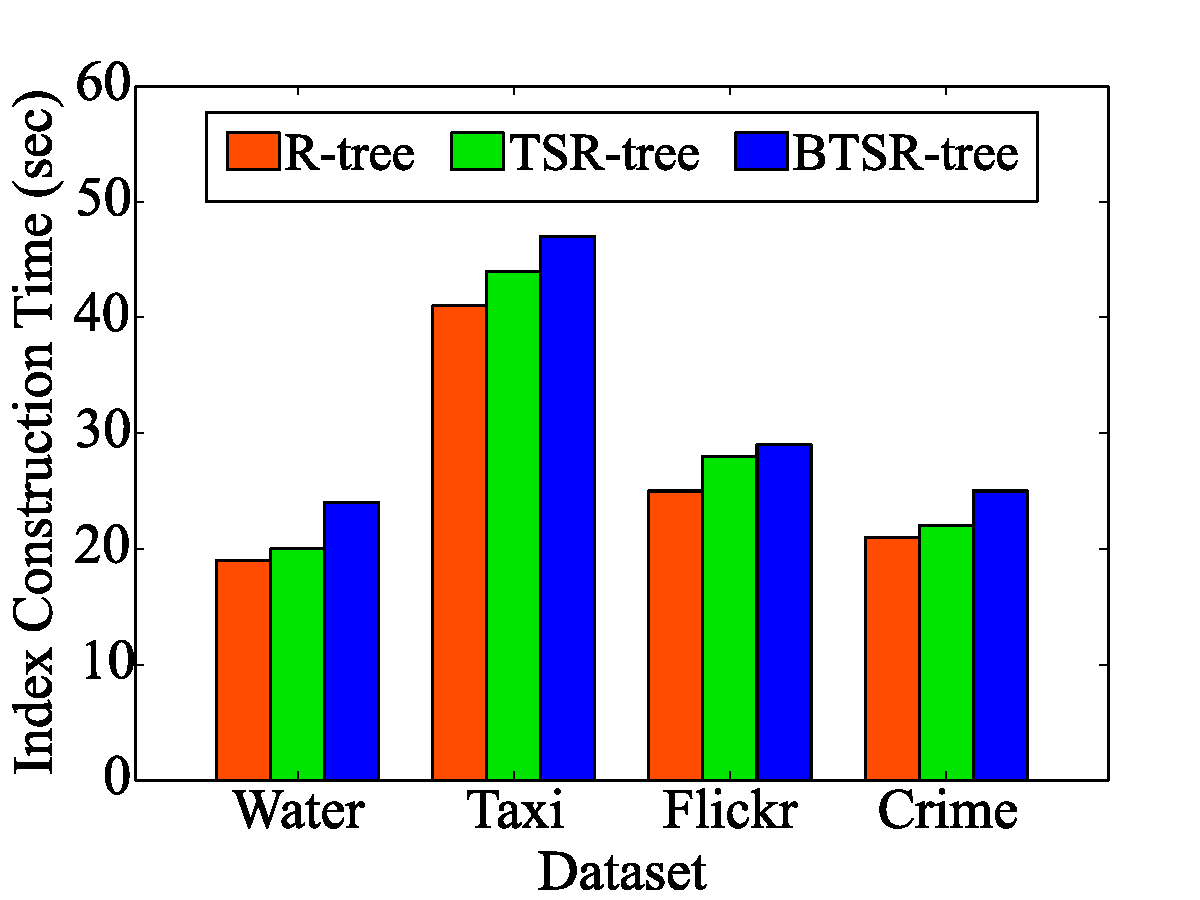
\includegraphics[width=0.45\textwidth]{figures/plots/index_time.pdf}\label{subfig:index_time}}
 \subfloat[Index size]{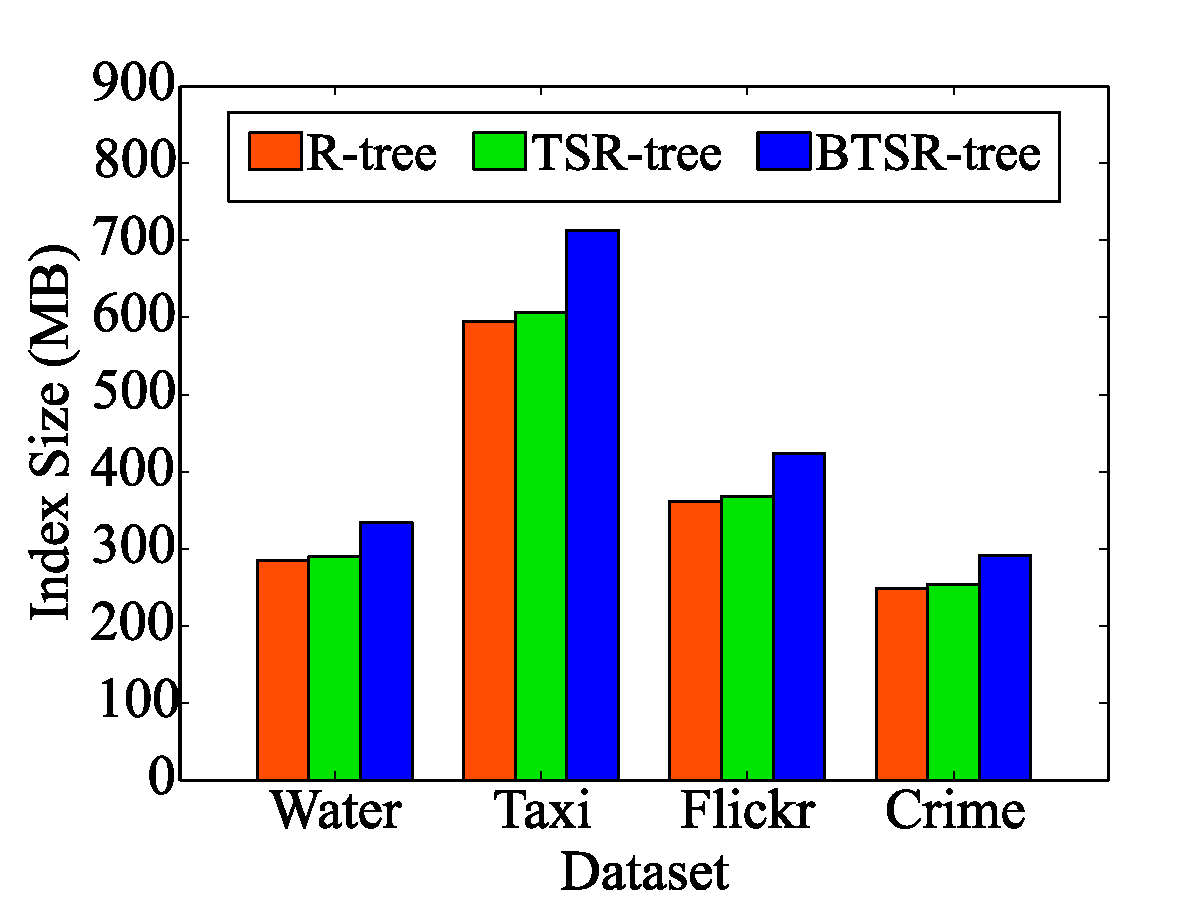
\includegraphics[width=0.45\textwidth]{figures/plots/index_size.pdf}\label{subfig:index_size}}
 \caption{Comparison of index construction time and size for each dataset.}
 \label{fig:index_construction}
\end{figure}

\subsection{Hybrid Similarity Search Query Performance}

We compare the percentage of nodes accessed by each index in each query. All measurements are average cost per query in each particular workload.

\paragraph{$Q_{bb}$.} Figure \ref{fig:query_qbb_theta_sp} illustrates the performance of the $Q_{bb}$ query on each dataset for varying spatial distance threshold ($\theta_{sp}$). Both the \tsr and the \btsr clearly outperform the standard R-tree in all datasets, with gains in performance increasing even further as the threshold $\theta_{sp}$ increases. The standard R-tree needs to access a significant amount of nodes as it can only prune in the spatial domain. As a result, it performs increasingly worse than the \tsr and the \btsr. Due to its tighter bounds, the \btsr manages to prune more nodes than the \tsr, especially for larger spatial threshold values.

\begin{figure}[!ht]
 \centering
 \subfloat[Water]{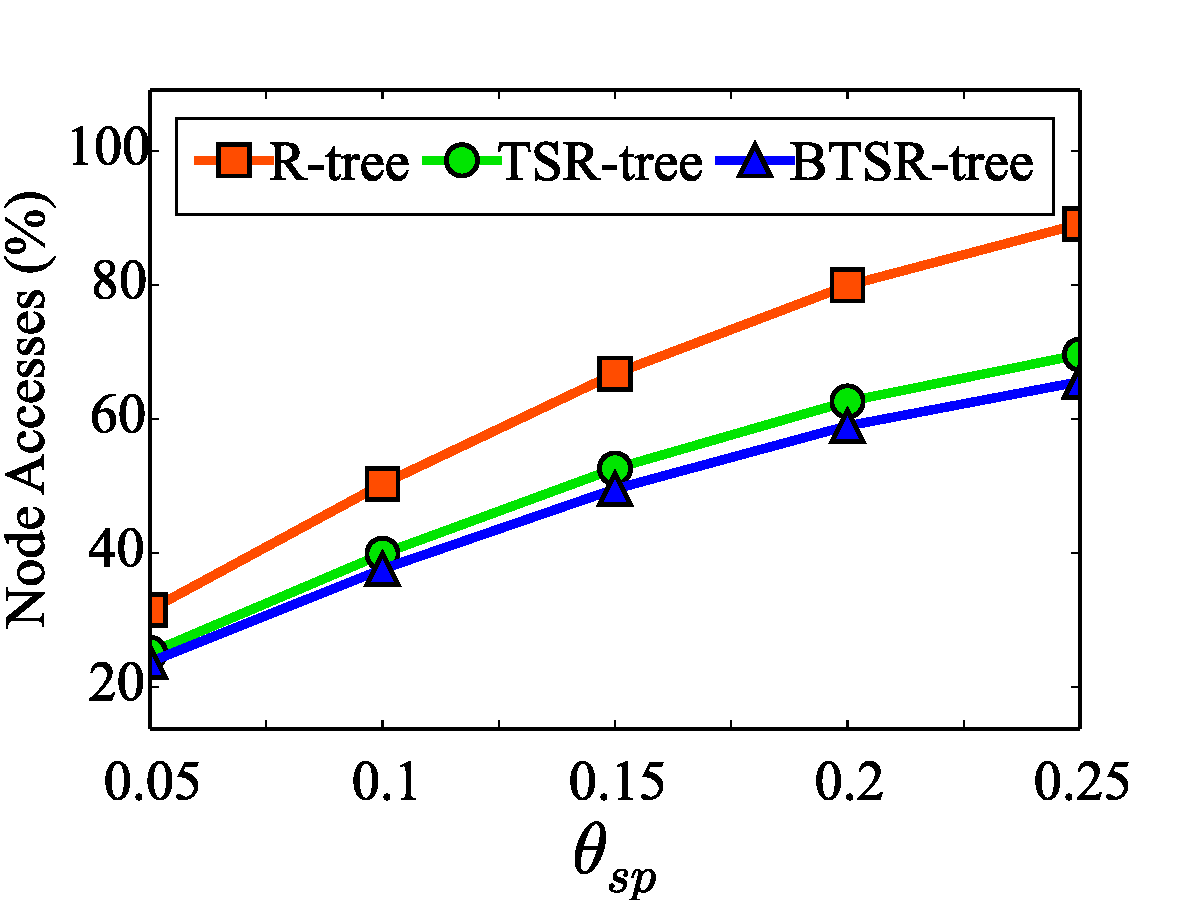
\includegraphics[width=0.45\textwidth]{figures/plots/water/qbb_theta_sp.pdf}\label{subfig:qbb_theta_sp_water}}
 \subfloat[Taxi]{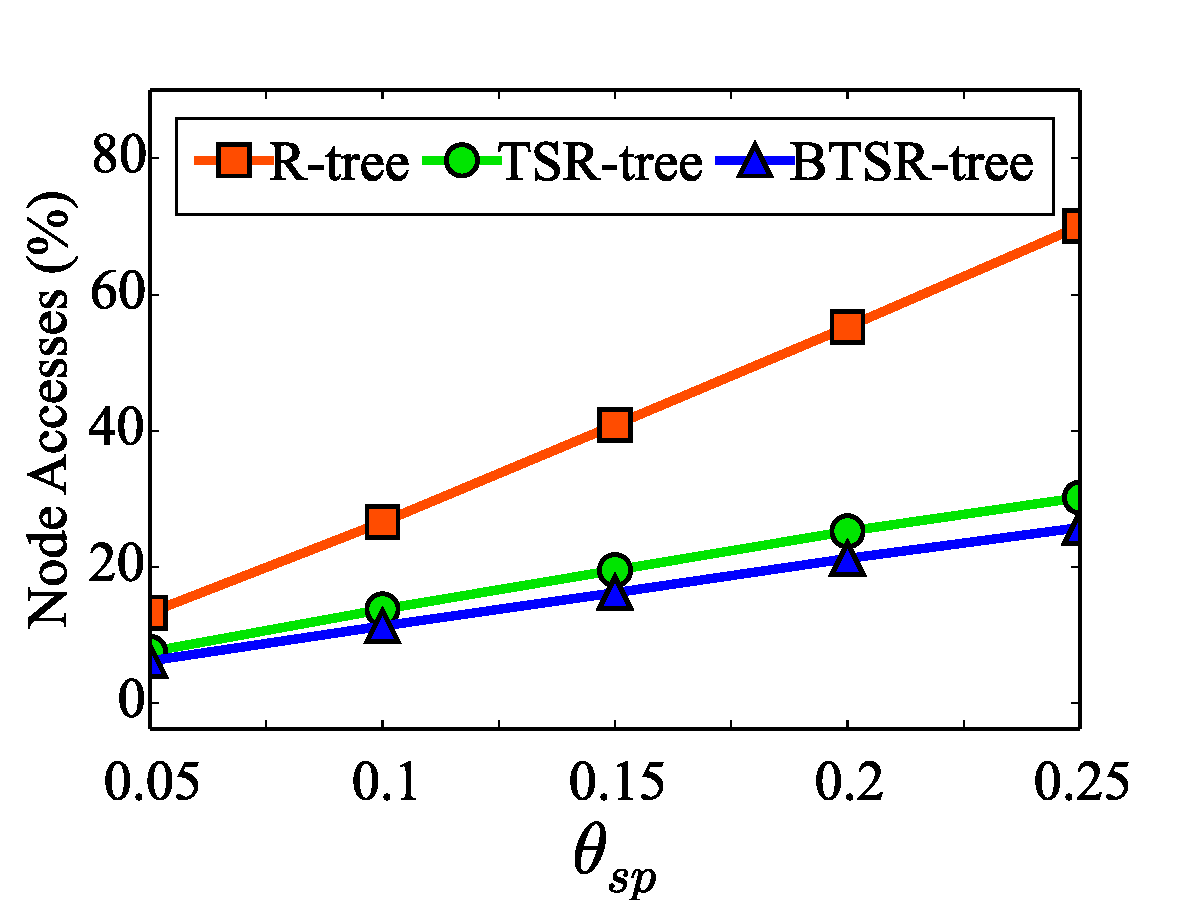
\includegraphics[width=0.45\textwidth]{figures/plots/taxi/qbb_theta_sp.pdf}\label{subfig:qbb_theta_sp_taxi}} \\
 \subfloat[Flickr]{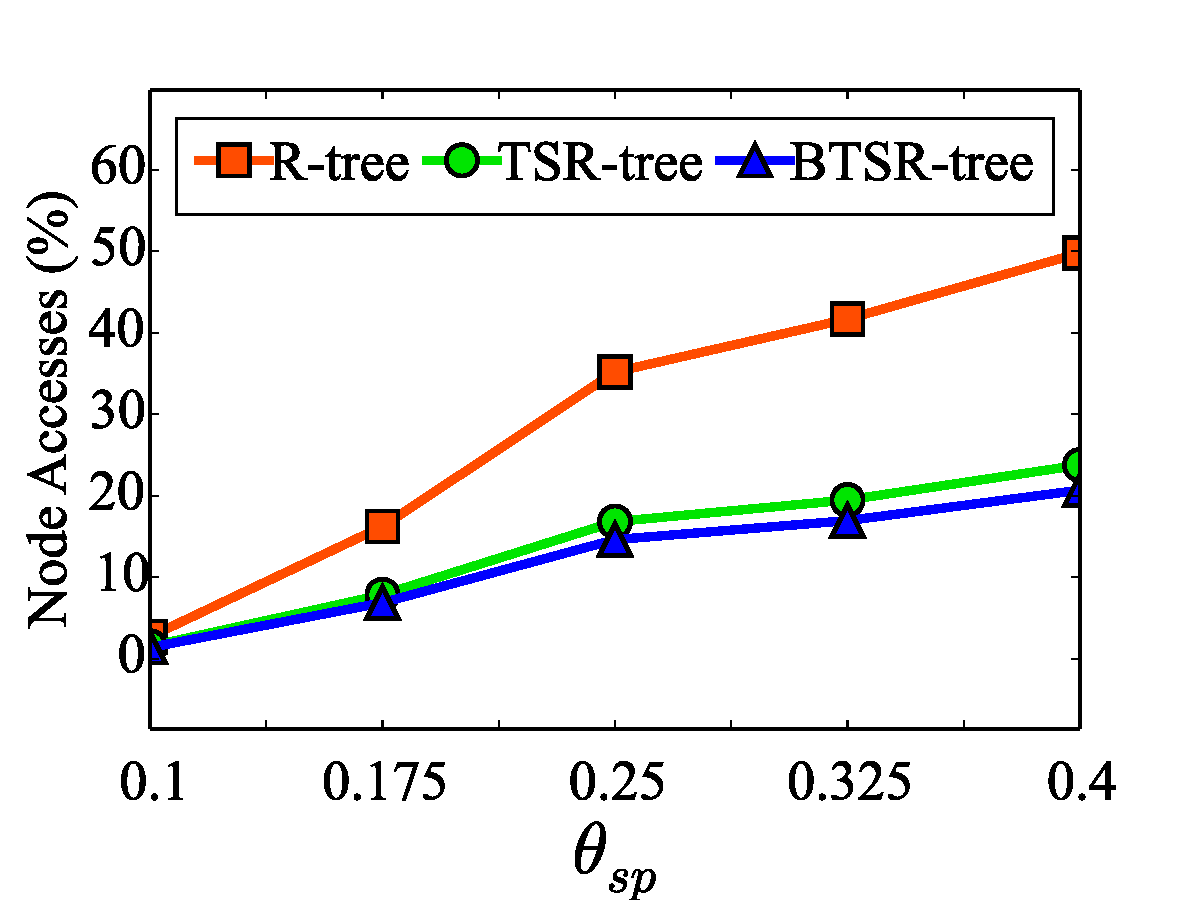
\includegraphics[width=0.45\textwidth]{figures/plots/flickr/qbb_theta_sp.pdf}\label{subfig:qbb_theta_sp_flickr}}
 \subfloat[Crime]{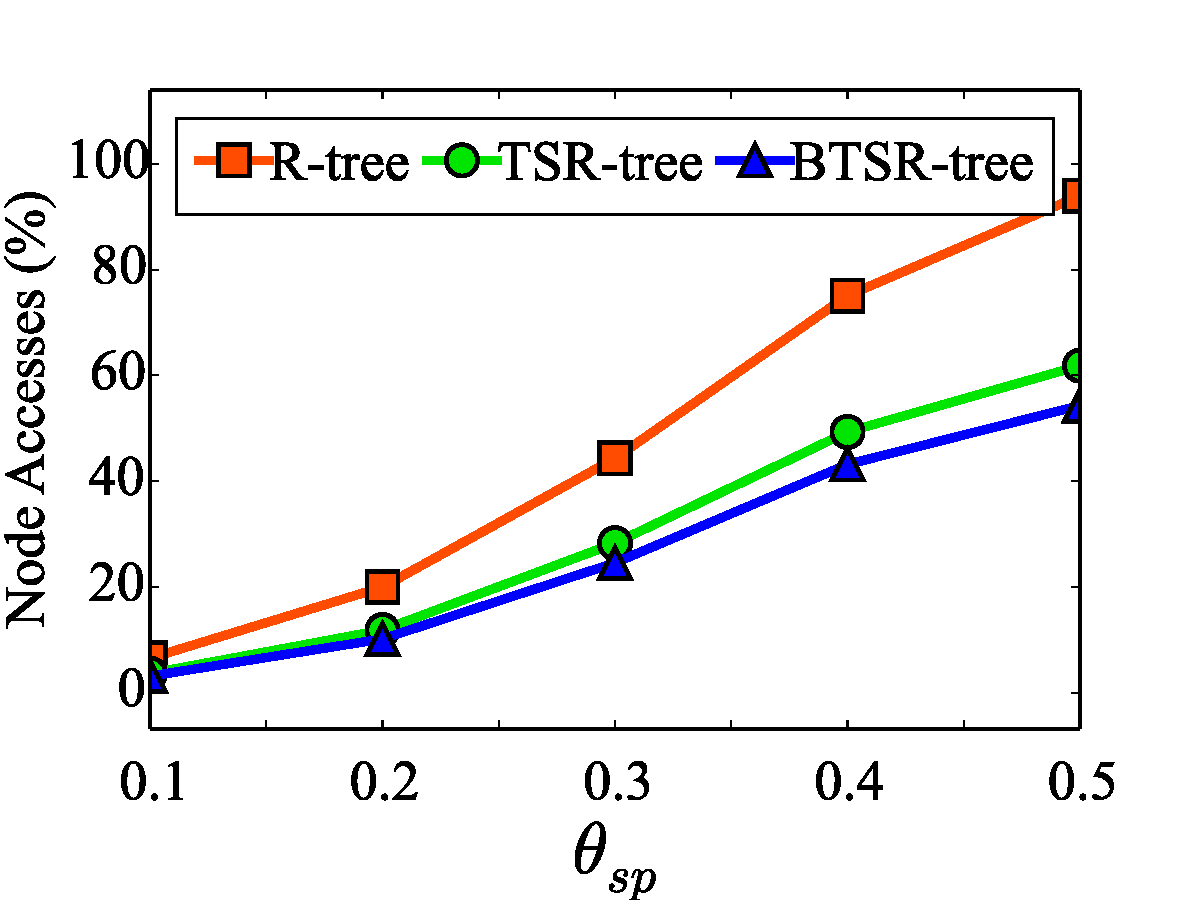
\includegraphics[width=0.45\textwidth]{figures/plots/crime/qbb_theta_sp.pdf}\label{subfig:qbb_theta_sp_crime}}
 \caption{Query $Q_{bb}(T_q, \theta_{sp}, \theta_{ts})$ with varying spatial distance threshold $\theta_{sp}$.}
 \label{fig:query_qbb_theta_sp}
\end{figure}

Obviously, increasing the time series threshold (Figure \ref{fig:query_qbb_theta_ts}) has absolutely no impact on the performance of the standard R-tree. On the contrary, the node accesses required by the \tsr and the \btsr are much lower. Nevertheless, these also increase with more relaxed $\theta_{ts}$, asymptotically reaching those of the R-tree. Performance of the \btsr is better for lower values of $\theta_{ts}$, as it allows more pruning thanks to the tighter bounds of bundles. It is apparent that the sensitivity of the threshold heavily depends on the dataset. Even slightly increasing $\theta_{ts}$ in the Taxi and Flickr datasets (Figure \ref{subfig:qbb_theta_ts_taxi} and \ref{subfig:qbb_theta_ts_flickr}), significantly affects performance of both the \tsr and the \btsr, as they are more sparse than the Water and Crime datasets (Figure \ref{subfig:qbb_theta_ts_water} and \ref{subfig:qbb_theta_ts_crime}), with a large number of time series having many zero values. Consequently, even a small increase in this threshold causes a larger amount of nodes to be probed.

\begin{figure}[!ht]
 \centering
 \subfloat[Water]{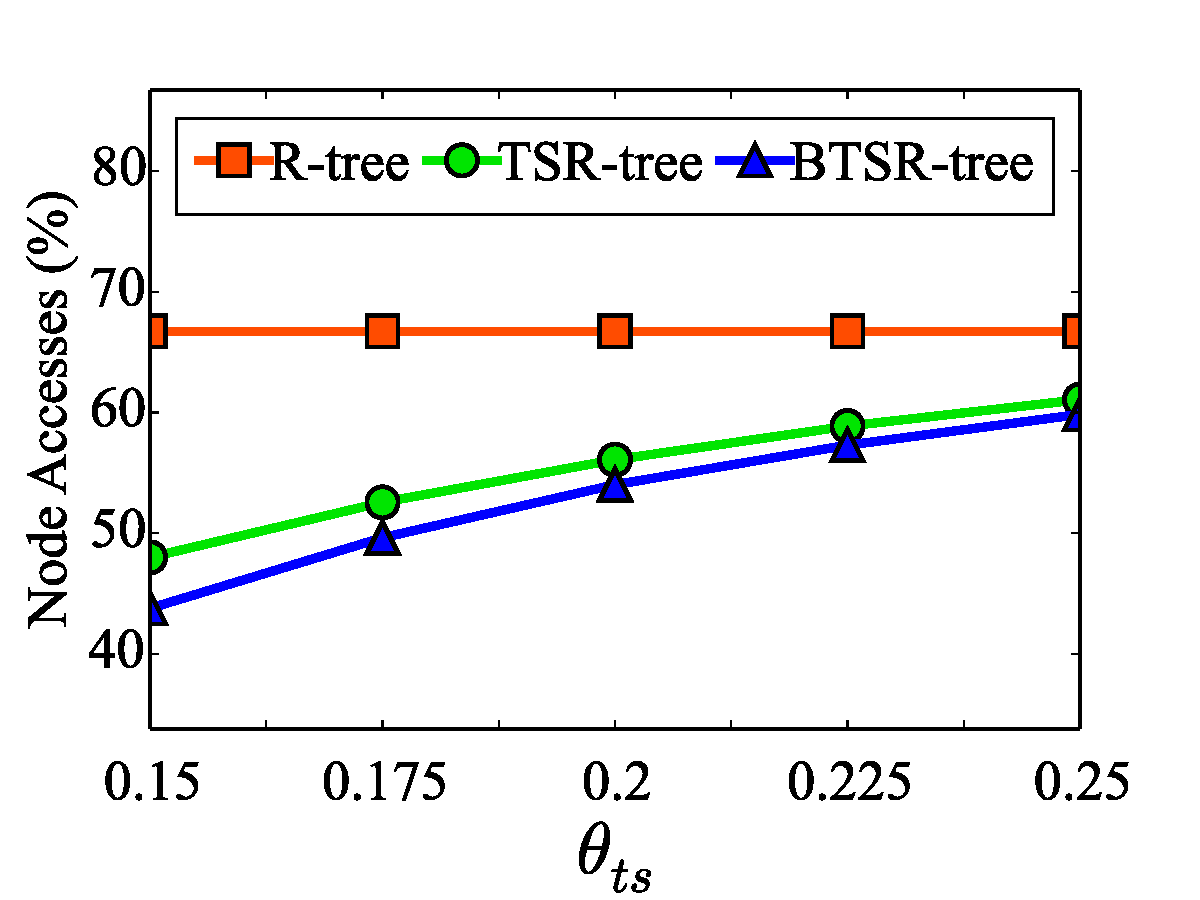
\includegraphics[width=0.45\textwidth]{figures/plots/water/qbb_theta_ts.pdf}\label{subfig:qbb_theta_ts_water}}
 \subfloat[Taxi]{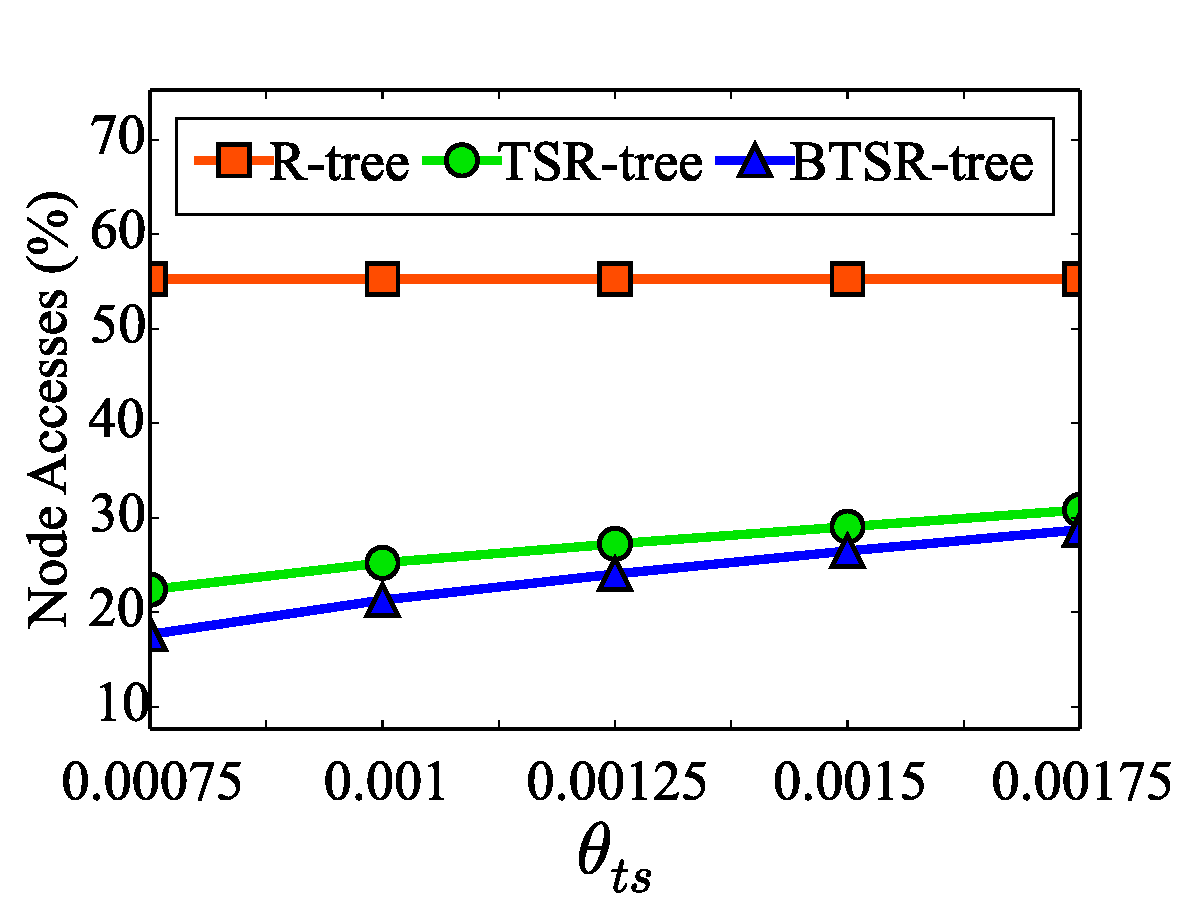
\includegraphics[width=0.45\textwidth]{figures/plots/taxi/qbb_theta_ts.pdf}\label{subfig:qbb_theta_ts_taxi}} \\
 \subfloat[Flickr]{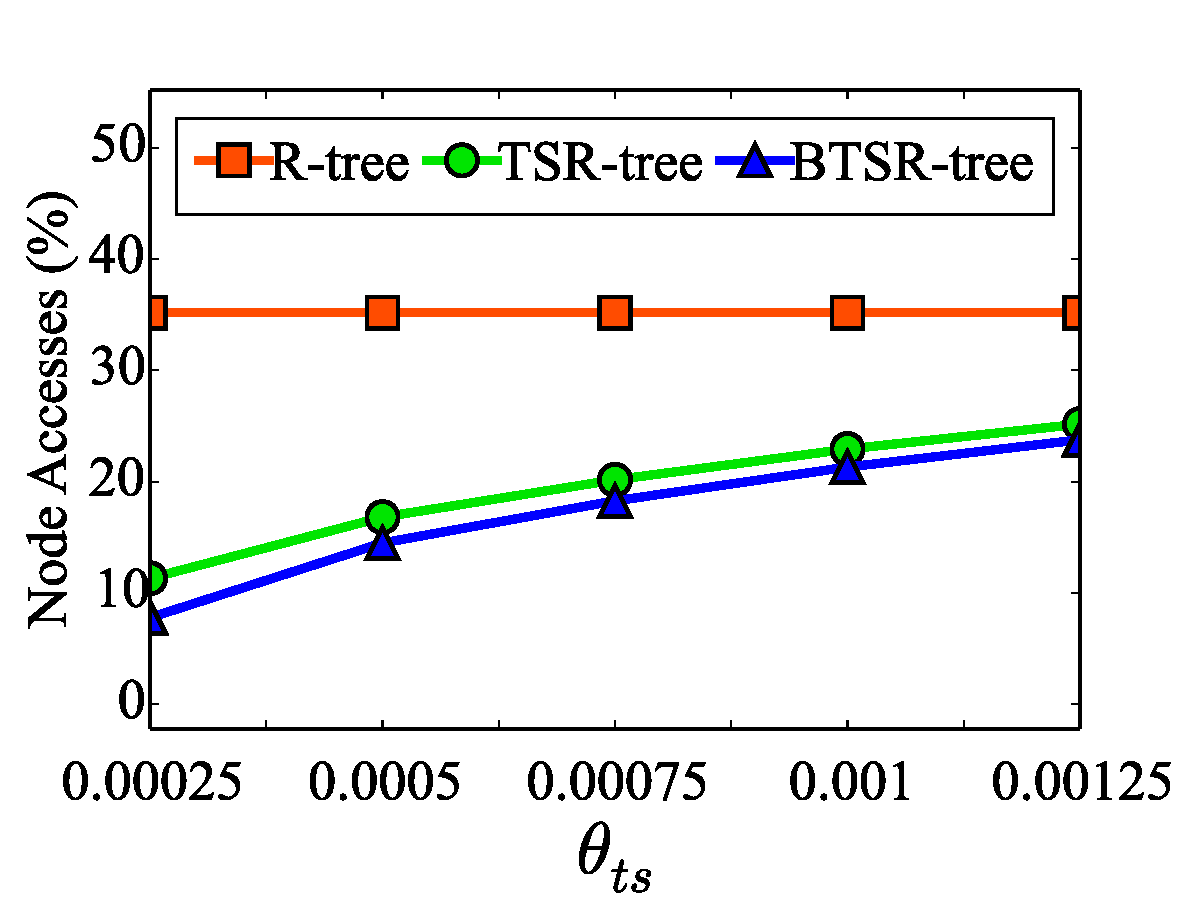
\includegraphics[width=0.45\textwidth]{figures/plots/flickr/qbb_theta_ts.pdf}\label{subfig:qbb_theta_ts_flickr}}
 \subfloat[Crime]{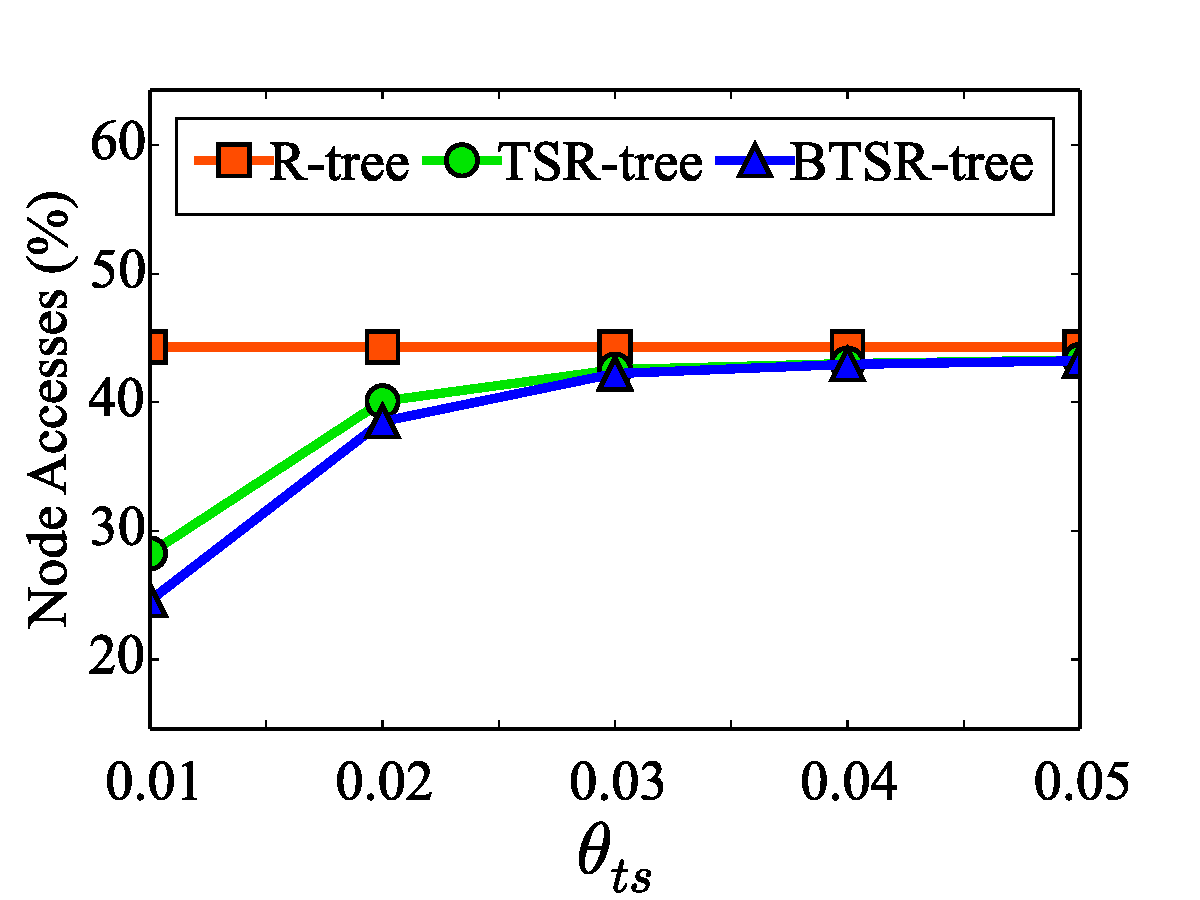
\includegraphics[width=0.45\textwidth]{figures/plots/crime/qbb_theta_ts.pdf}\label{subfig:qbb_theta_ts_crime}}
 \caption{Query $Q_{bb}(T_q, \theta_{sp}, \theta_{ts})$ with varying time series distance threshold $\theta_{ts}$.}
 \label{fig:query_qbb_theta_ts}
\end{figure}

\paragraph{$Q_{kb}$.} Performance of $Q_{kb}$ for varying number $k$ of results is depicted in Figure \ref{fig:query_qkb_k}.  In all cases, both the \tsr and the \btsr cope better compared to the standard R-tree. Varying the number $k$  of results does not significantly affect performance, as nearby elements tend to have similar time series values and all required results are found in close distance. This is an interesting insight, especially for the Water dataset, which suggests that neighboring households tend to have similar water consumption. The R-tree performs really poor in the Crime dataset (Figure \ref{subfig:qkb_k_crime}), requiring a full traversal ($100\%$ of its nodes), as the sought number of results cannot be found. This is not the case with the \tsr and the \btsr, respectively accessing $65\%$ and $58\%$ of their nodes due to their effective pruning in the time series domain.

\begin{figure}[!ht]
 \centering
 \subfloat[Water]{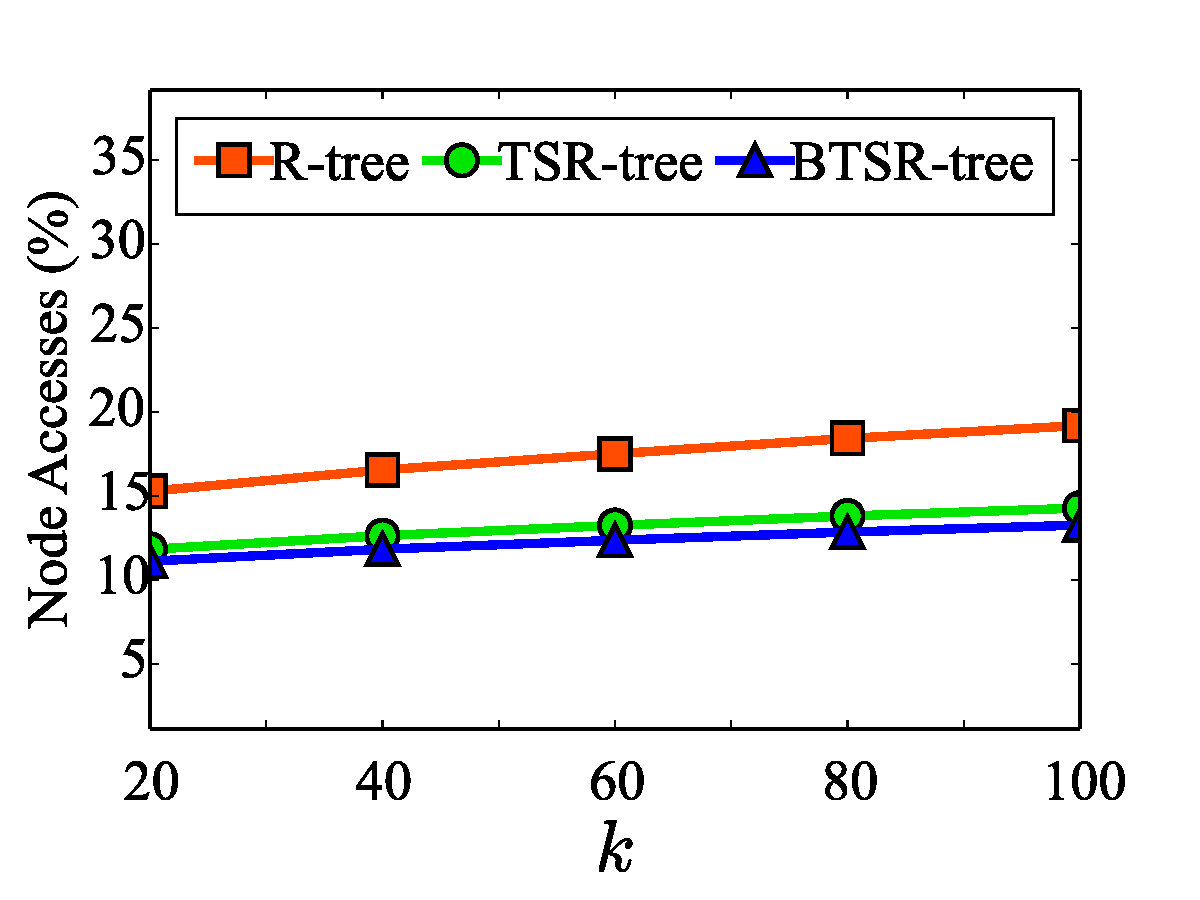
\includegraphics[width=0.45\textwidth]{figures/plots/water/qkb_k.pdf}\label{subfig:qkb_k_water}}
 \subfloat[Taxi]{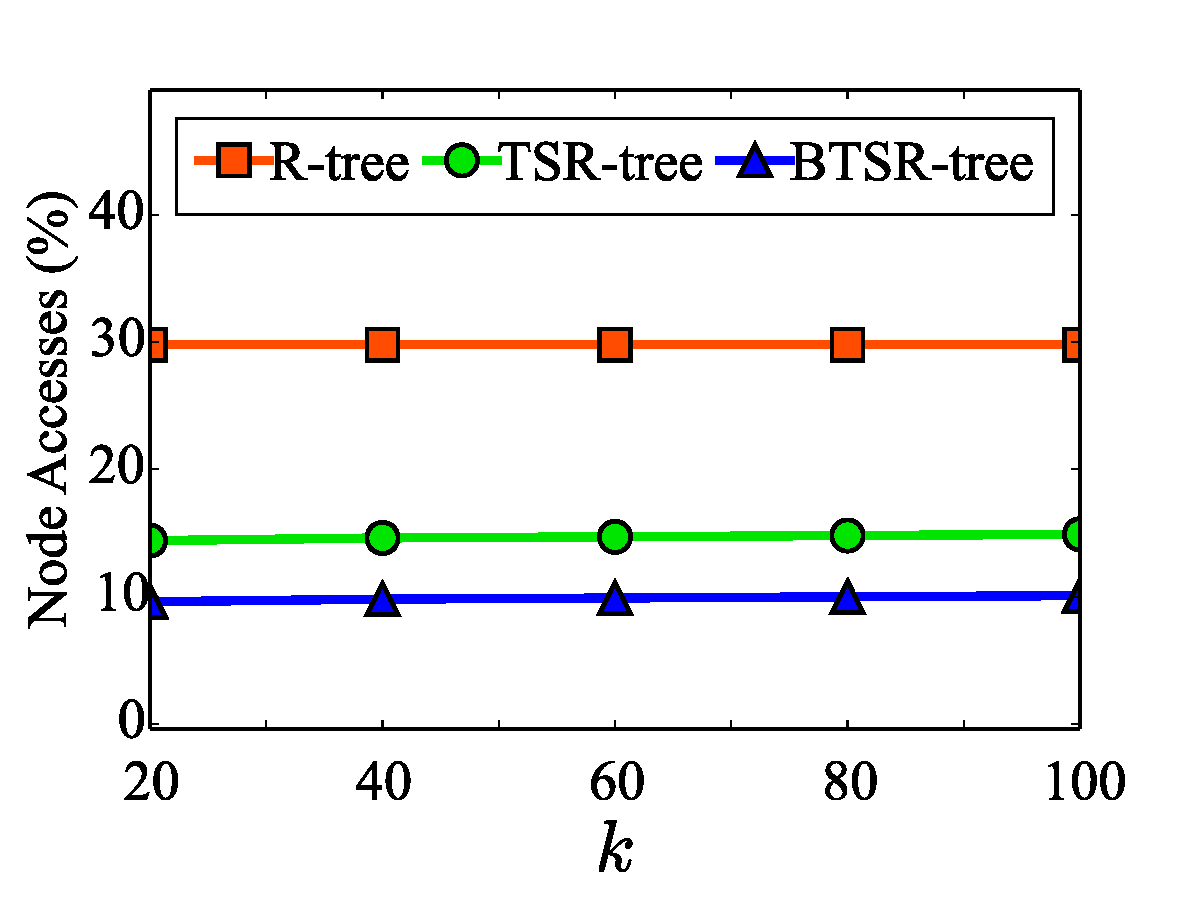
\includegraphics[width=0.45\textwidth]{figures/plots/taxi/qkb_k.pdf}\label{subfig:qkb_k_taxi}} \\
 \subfloat[Flickr]{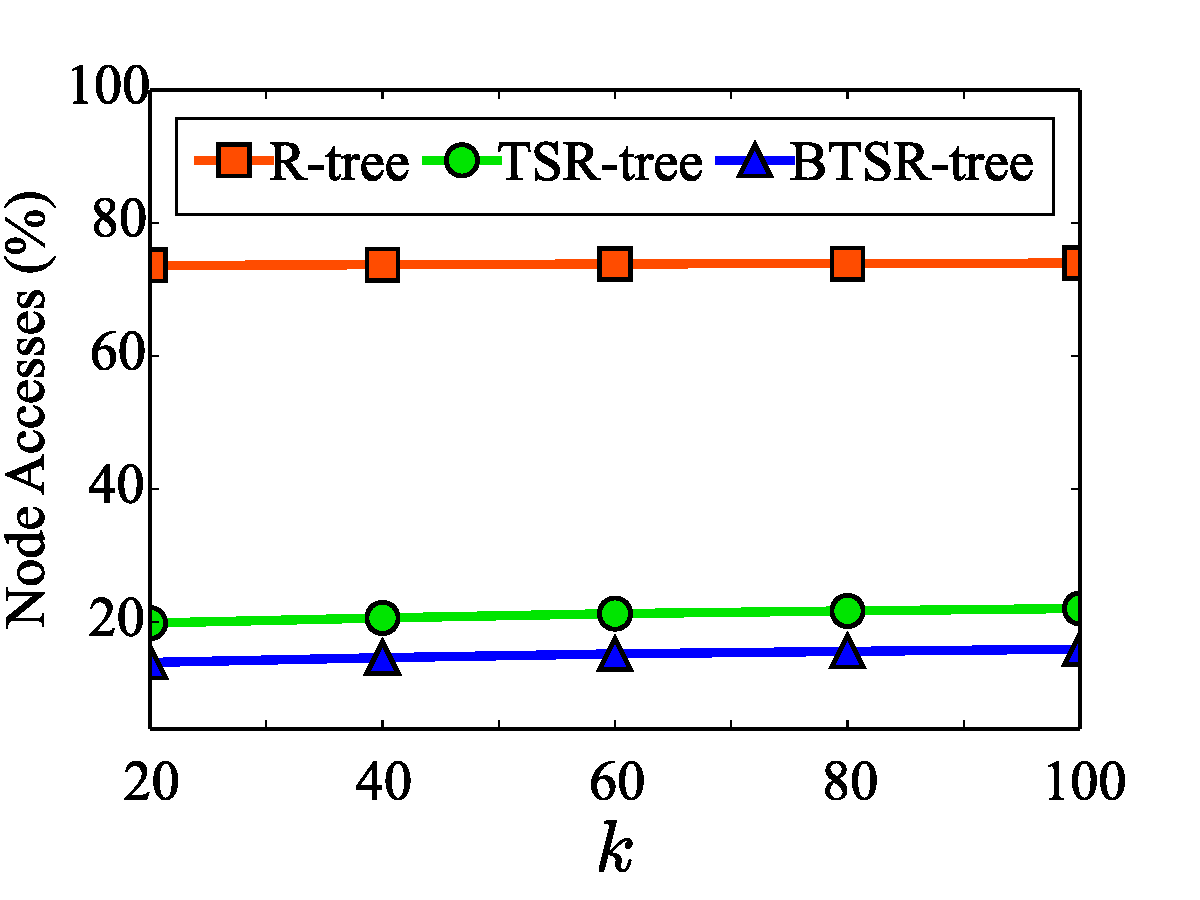
\includegraphics[width=0.45\textwidth]{figures/plots/flickr/qkb_k.pdf}\label{subfig:qkb_k_flickr}}
 \subfloat[Crime]{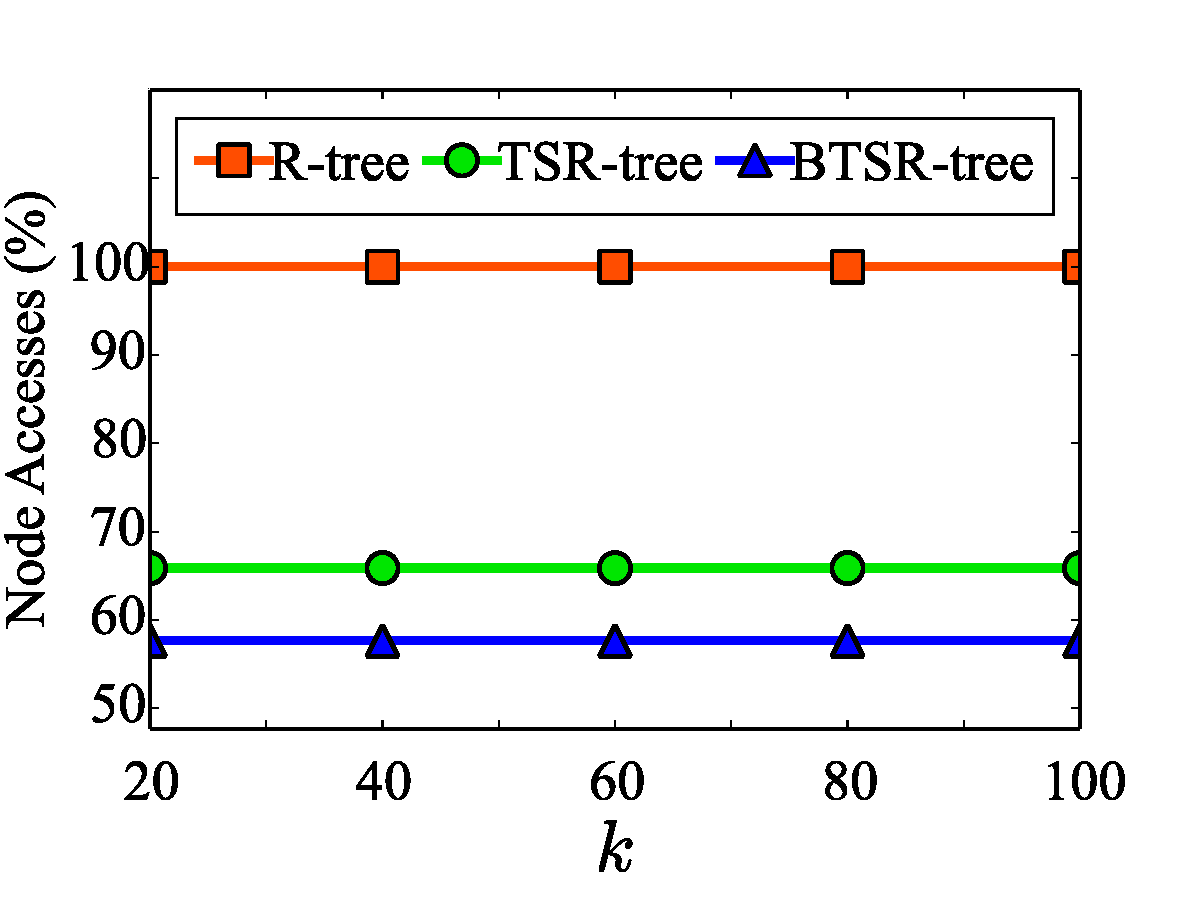
\includegraphics[width=0.45\textwidth]{figures/plots/crime/qkb_k.pdf}\label{subfig:qkb_k_crime}}
 \caption{Query $Q_{kb}(T_q, k, \theta_{ts})$ with varying number $k$ of results.}
 \label{fig:query_qkb_k}
\end{figure}

Increasing the time series threshold $\theta_{ts}$ (Figure \ref{fig:query_qkb_theta_ts}) in $Q_{kb}$, improves performance of the R-tree and it is sometimes competitive to that of the \tsr and the \btsr, as more nearby elements qualify as results and are thus quickly found. However, this is strongly influenced by dataset characteristics. For the Taxi dataset (Figure \ref{subfig:qkb_theta_ts_taxi}), node accesses in the R-tree are similar for different values of $\theta_{ts}$, but performance for the \btsr slightly decreases with higher threshold values. Indeed, relaxing this threshold effectively allows more tolerance in the similarity of time series and thus, extra nodes need to be visited for checking.

\begin{figure}[!ht]
	\centering
	\subfloat[Water]{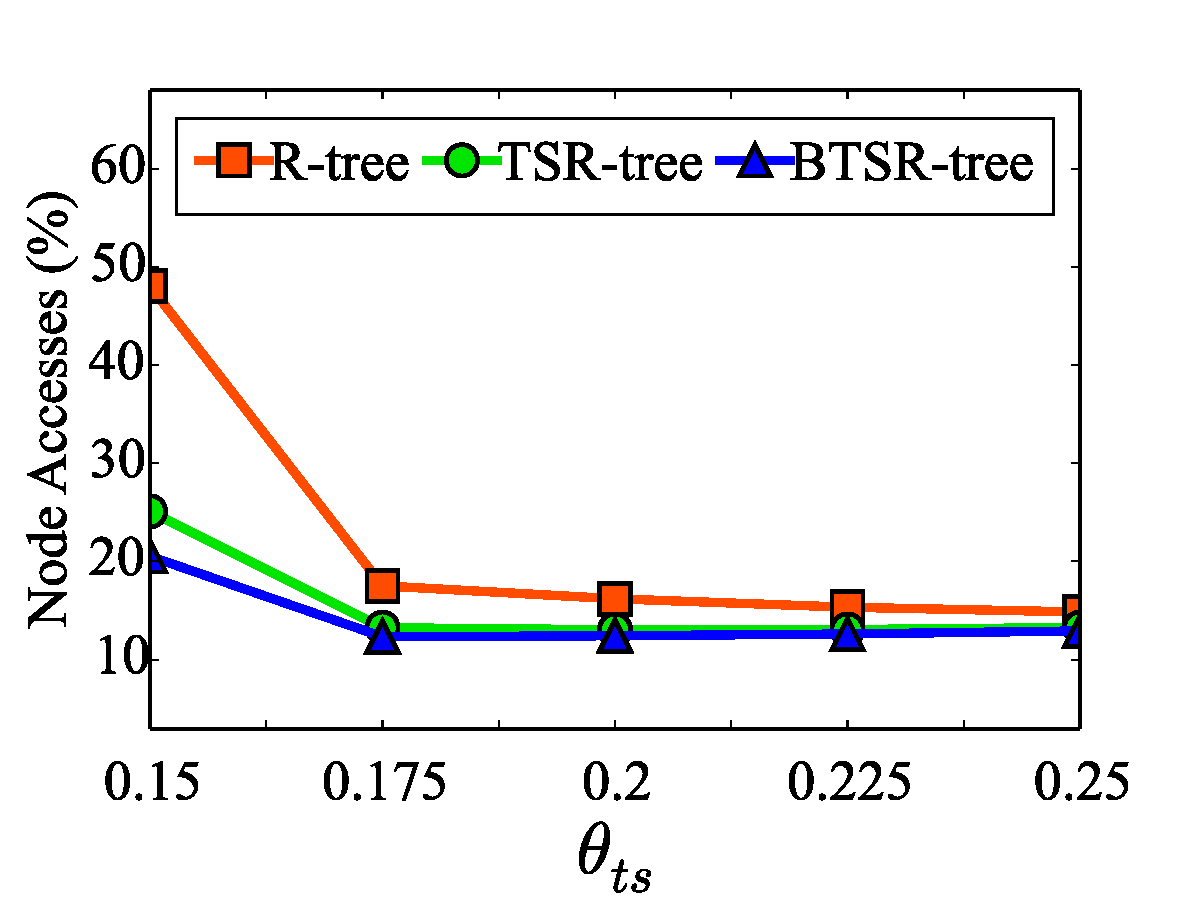
\includegraphics[width=0.45\textwidth]{figures/plots/water/qkb_theta_ts.pdf}\label{subfig:qkb_theta_ts_water}}
	\subfloat[Taxi]{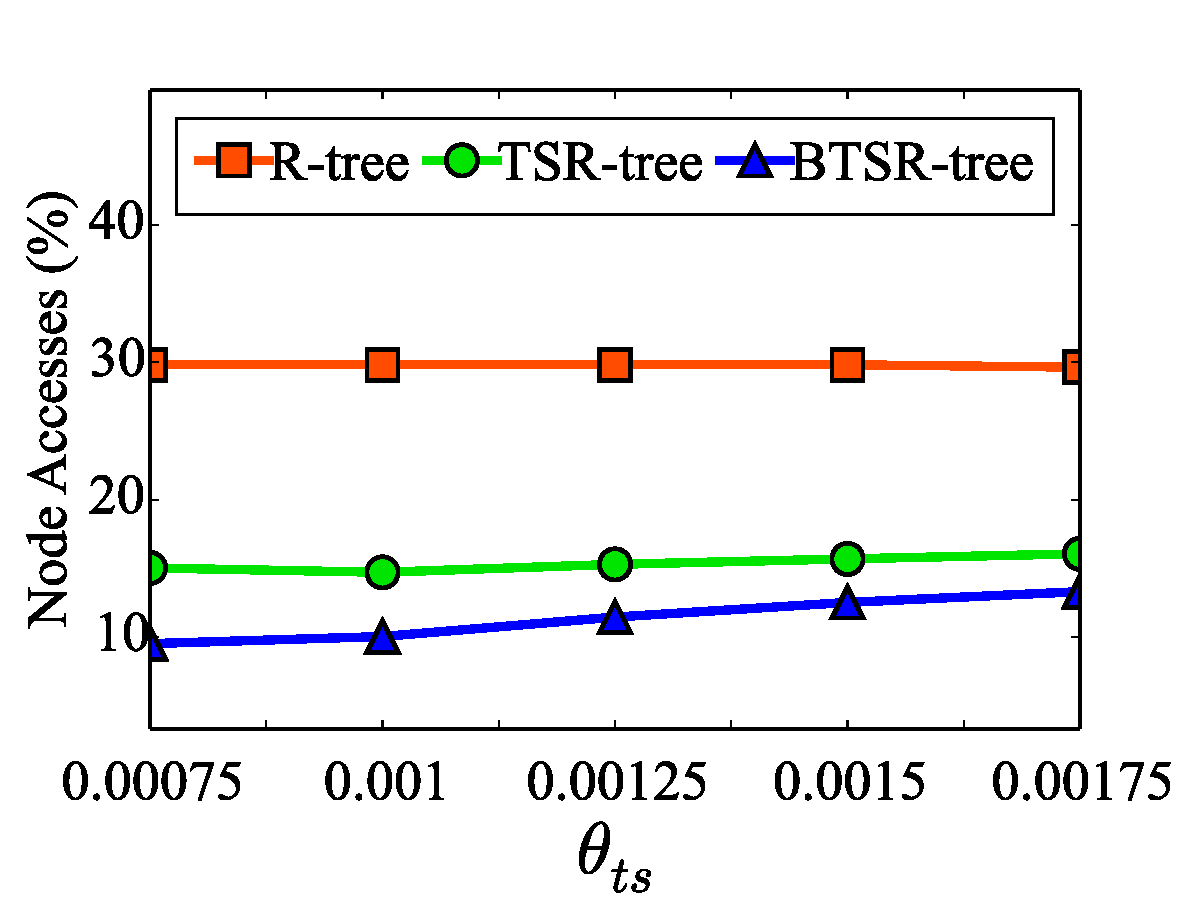
\includegraphics[width=0.45\textwidth]{figures/plots/taxi/qkb_theta_ts.pdf}\label{subfig:qkb_theta_ts_taxi}} \\
	\subfloat[Flickr]{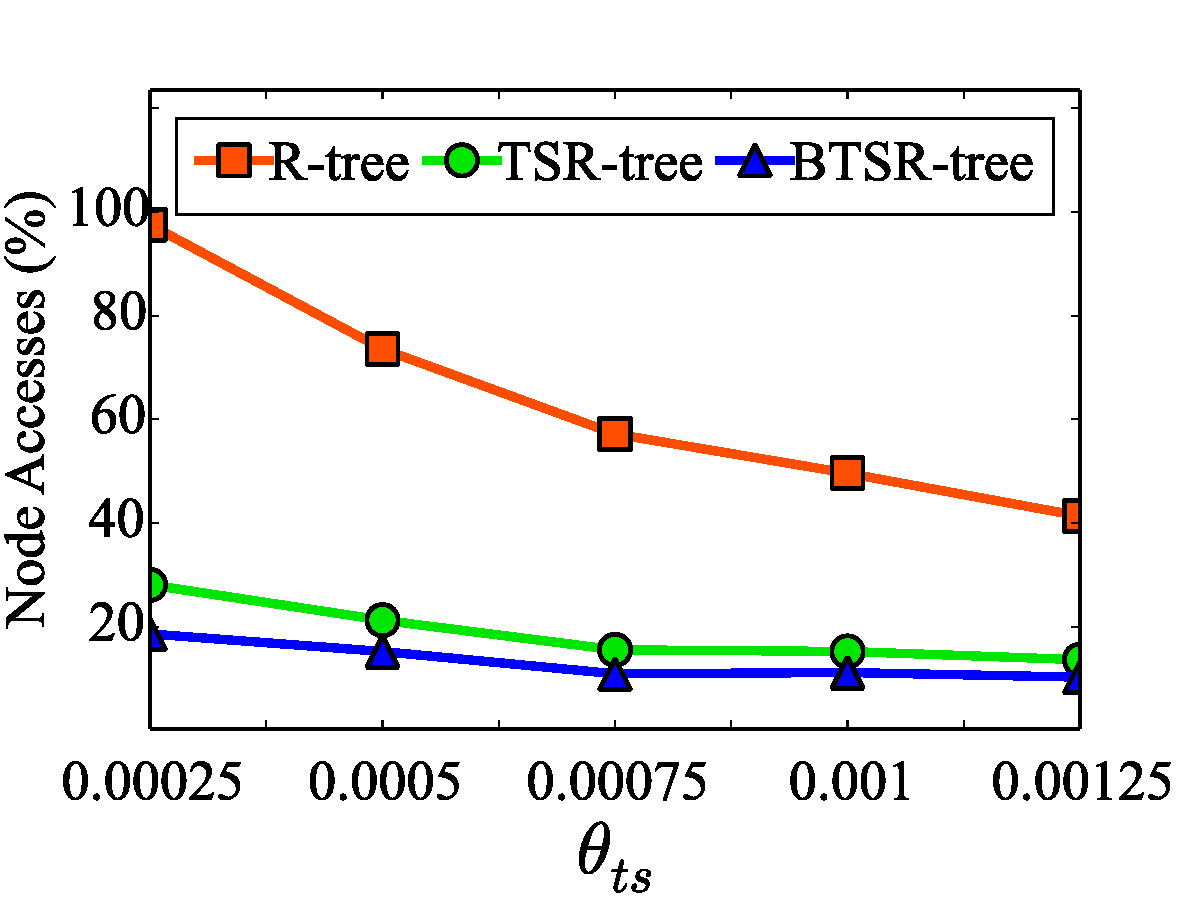
\includegraphics[width=0.45\textwidth]{figures/plots/flickr/qkb_theta_ts.pdf}\label{subfig:qkb_theta_ts_flickr}}
	\subfloat[Crime]{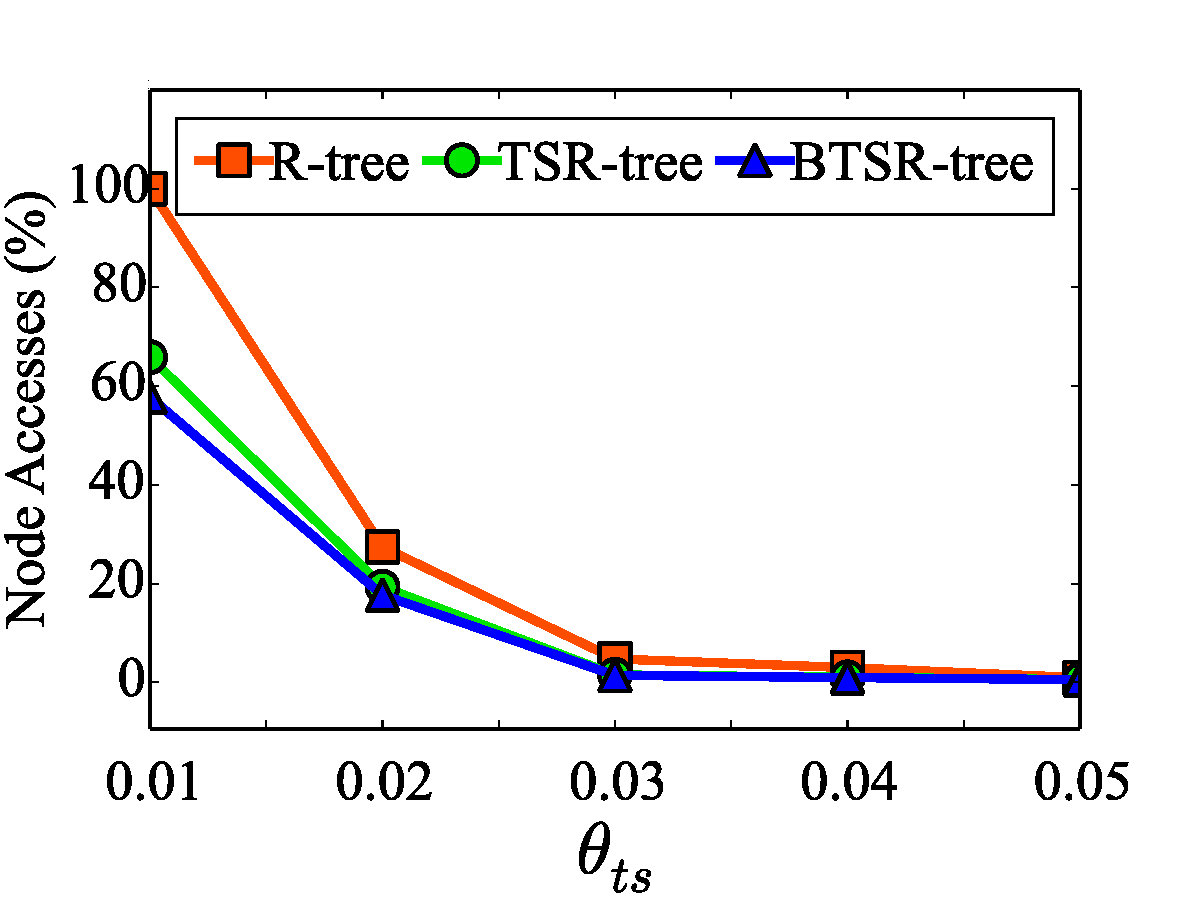
\includegraphics[width=0.45\textwidth]{figures/plots/crime/qkb_theta_ts.pdf}\label{subfig:qkb_theta_ts_crime}}
	\caption{Query $Q_{kb}(T_q, k, \theta_{ts})$ with varying time series distance threshold $\theta_{ts}$.}
	\label{fig:query_qkb_theta_ts}
\end{figure}


\paragraph{$Q_{bk}$.} Varying the number $k$ of results in the $Q_{bk}$ query (Figure \ref{fig:query_qbk_k}), shows similar behavior to the $Q_{kb}$ query. Similar time series are located close to each other, so $k$ results are quickly obtained once the first qualifying time series is retrieved. The R-tree is always significantly outperformed by the \tsr and \btsr;  the effect is less apparent in the Crime dataset (Figure \ref{subfig:qbk_k_crime}).

\begin{figure}[!ht]
	\centering
	\subfloat[Water]{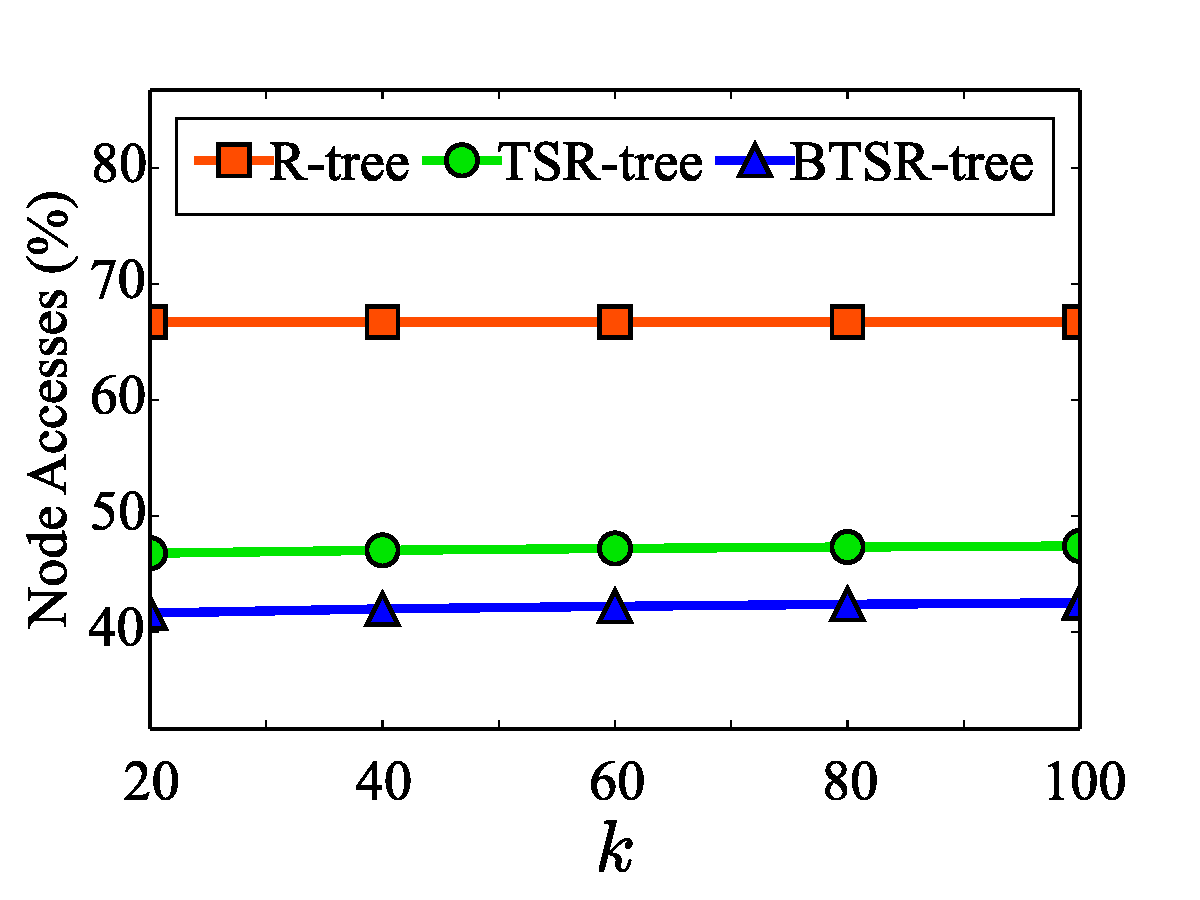
\includegraphics[width=0.45\textwidth]{figures/plots/water/qbk_k.pdf}\label{subfig:qbk_k_water}}
	\subfloat[Taxi]{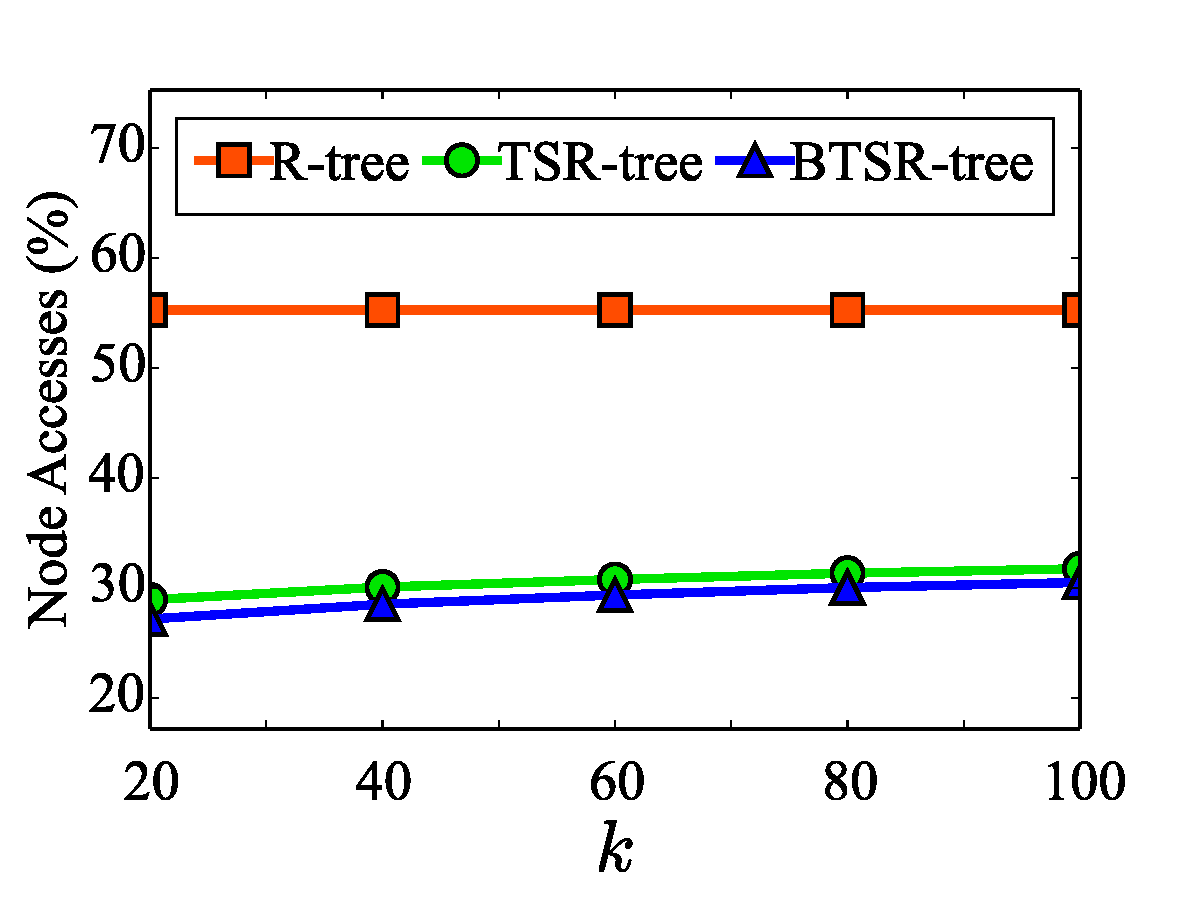
\includegraphics[width=0.45\textwidth]{figures/plots/taxi/qbk_k.pdf}\label{subfig:qbk_k_taxi}} \\
	\subfloat[Flickr]{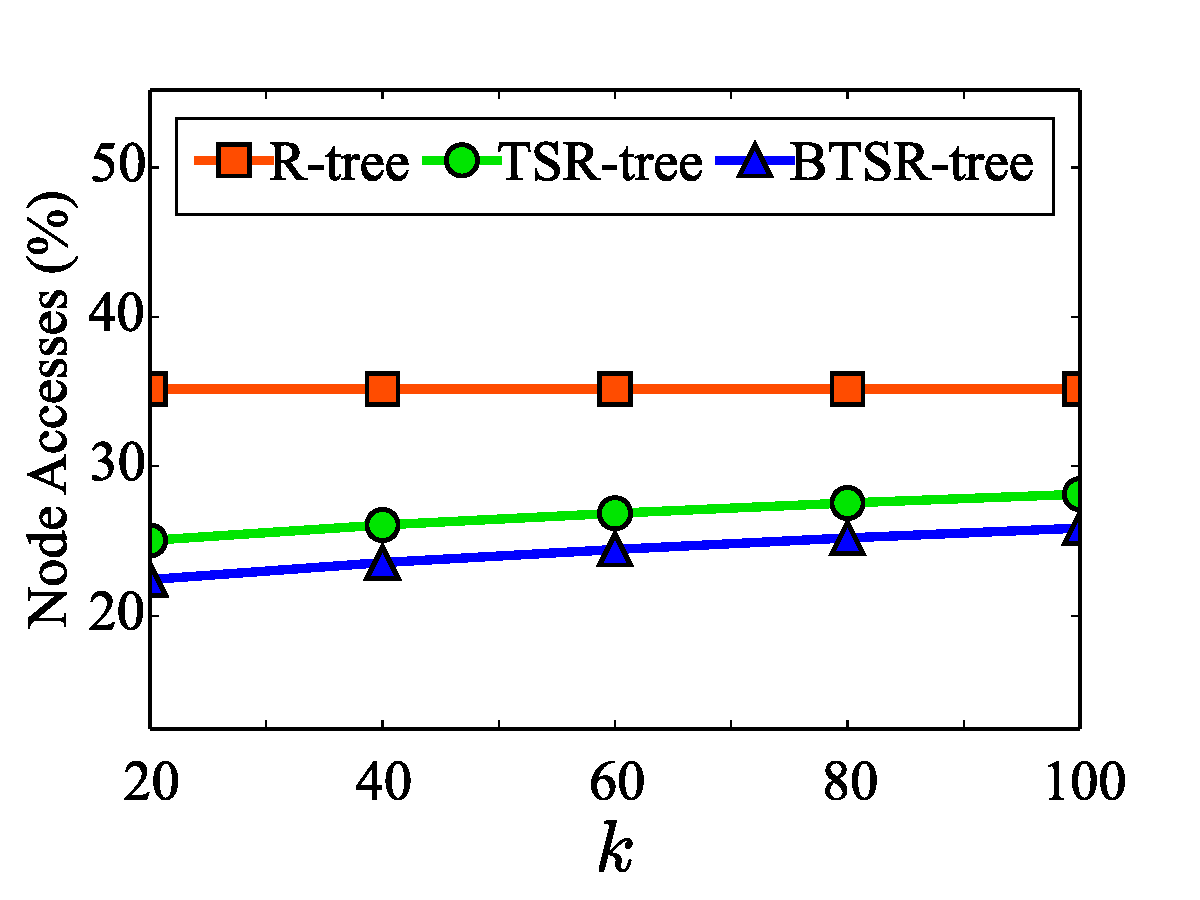
\includegraphics[width=0.45\textwidth]{figures/plots/flickr/qbk_k.pdf}\label{subfig:qbk_k_flickr}}
	\subfloat[Crime]{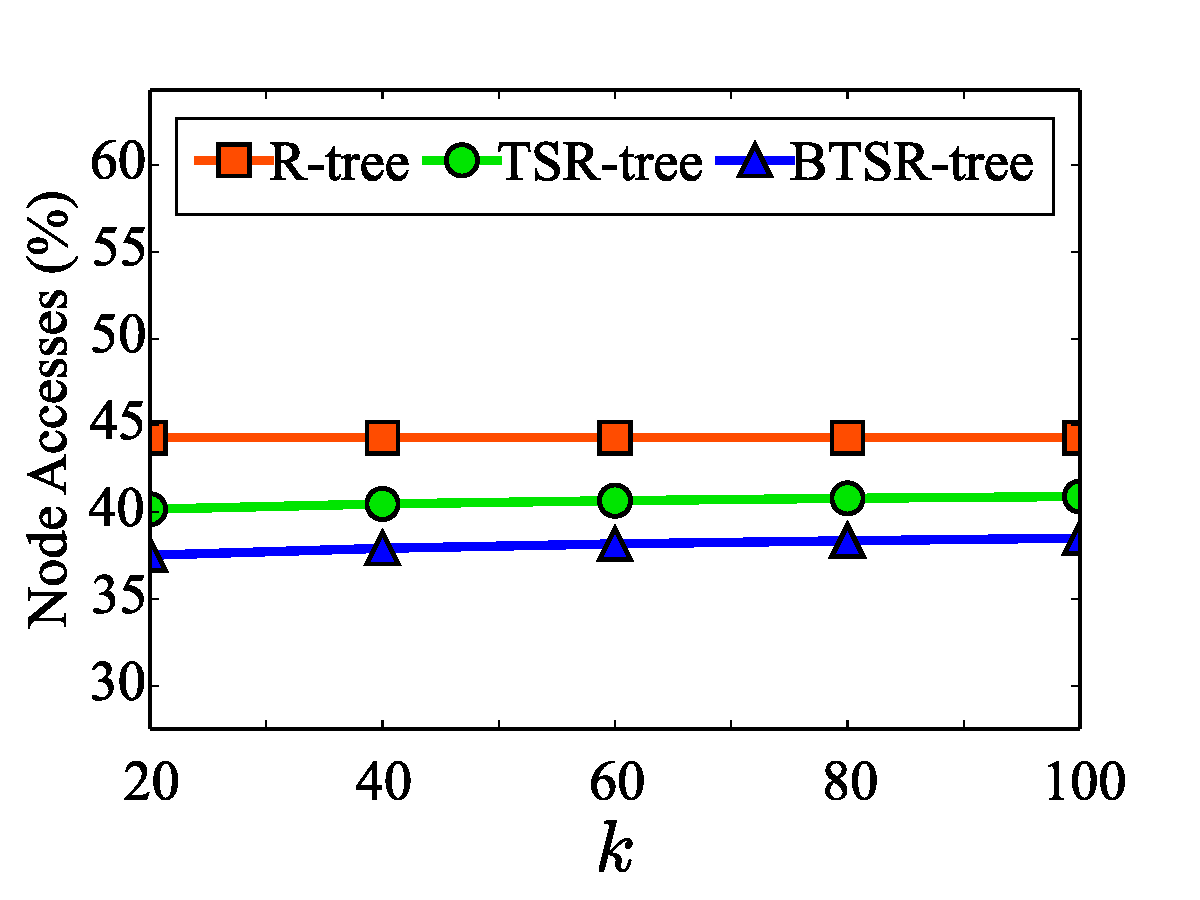
\includegraphics[width=0.45\textwidth]{figures/plots/crime/qbk_k.pdf}\label{subfig:qbk_k_crime}}
	\caption{Query $Q_{bk}(T_q, \theta_{sp}, k)$ with varying number $k$ of results.}
	\label{fig:query_qbk_k}
\end{figure}

Figure \ref{fig:query_qbk_theta_sp} illustrates performance of the $Q_{bk}$ query for varying spatial distance threshold ($\theta_{sp}$). The significantly better performance of the \tsr and the \btsr is also apparent here, with the difference getting more pronounced with larger thresholds (i.e., wider radii). This advantage is less manifest in the Crime dataset (Figure \ref{subfig:qbk_theta_sp_crime}) because the applied thresholds cover increasingly larger spatial areas (practically the entire dataset for $\theta_{sp} =0.5$), thus more nodes need to be examined in order to identify the $k$ results. In the Taxi dataset, the performance improvement of the \btsr compared to the \tsr is smaller due to data sparsity, which diminishes the pruning effect of bundles in the nodes of the \btsr.

\begin{figure}[!ht]
	\centering
	\subfloat[Water]{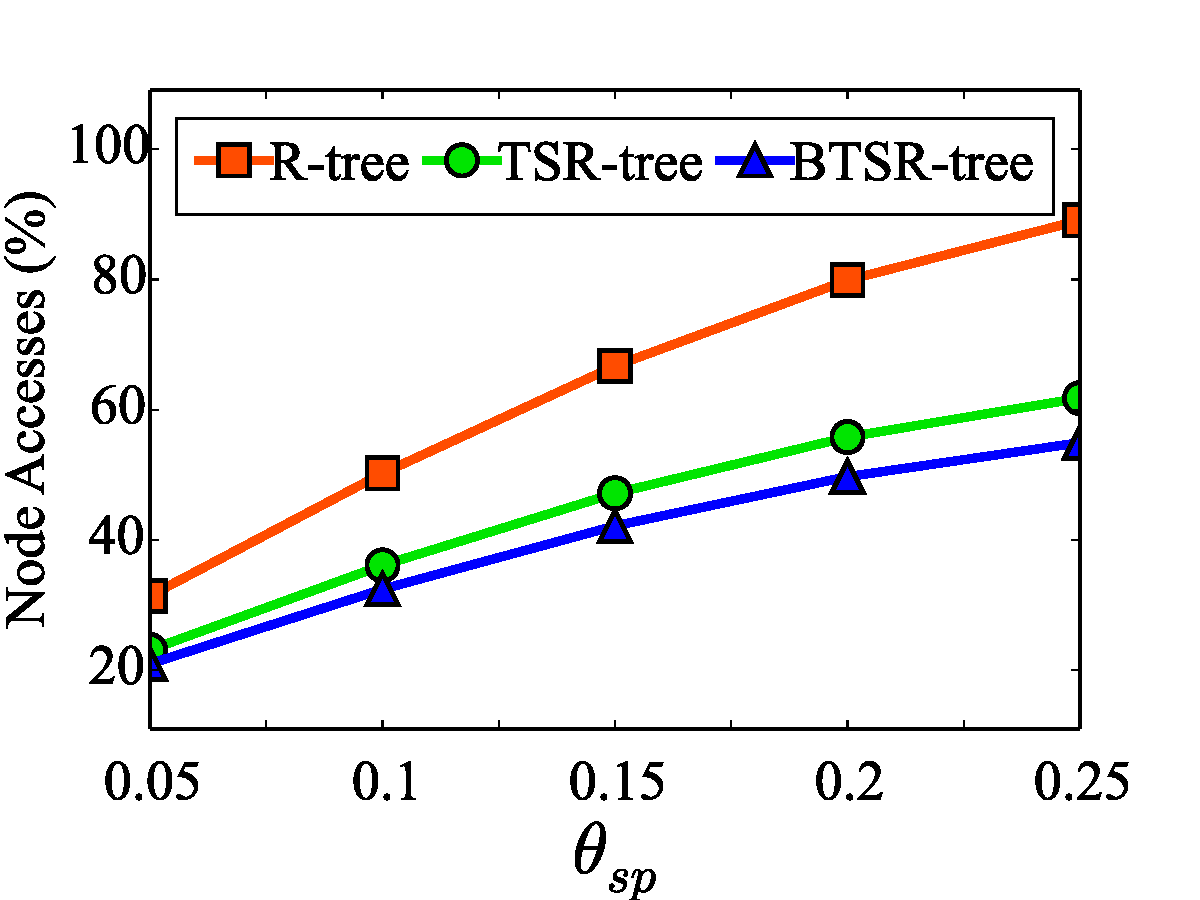
\includegraphics[width=0.45\textwidth]{figures/plots/water/qbk_theta_sp.pdf}\label{subfig:qbk_theta_sp_water}}
	\subfloat[Taxi]{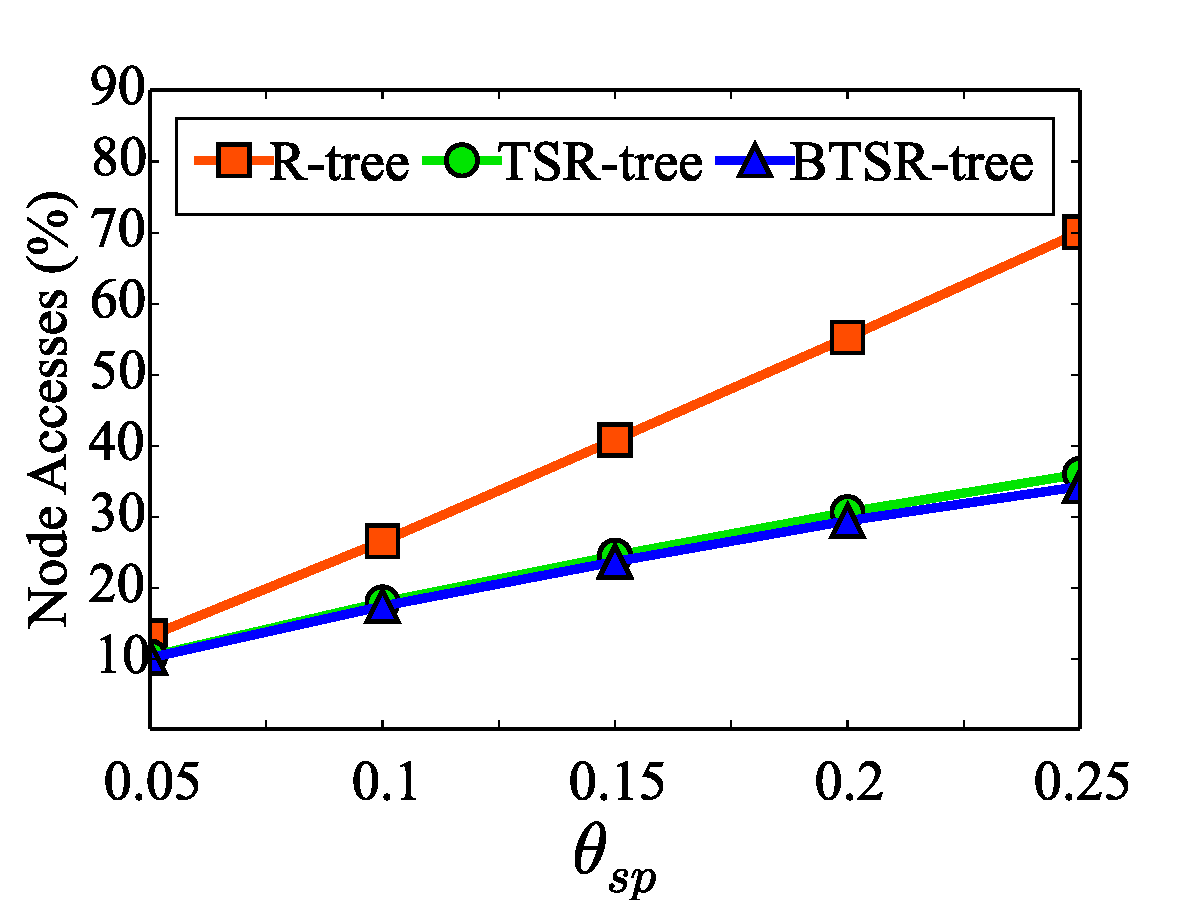
\includegraphics[width=0.45\textwidth]{figures/plots/taxi/qbk_theta_sp.pdf}\label{subfig:qbk_theta_sp_taxi}} \\
	\subfloat[Flickr]{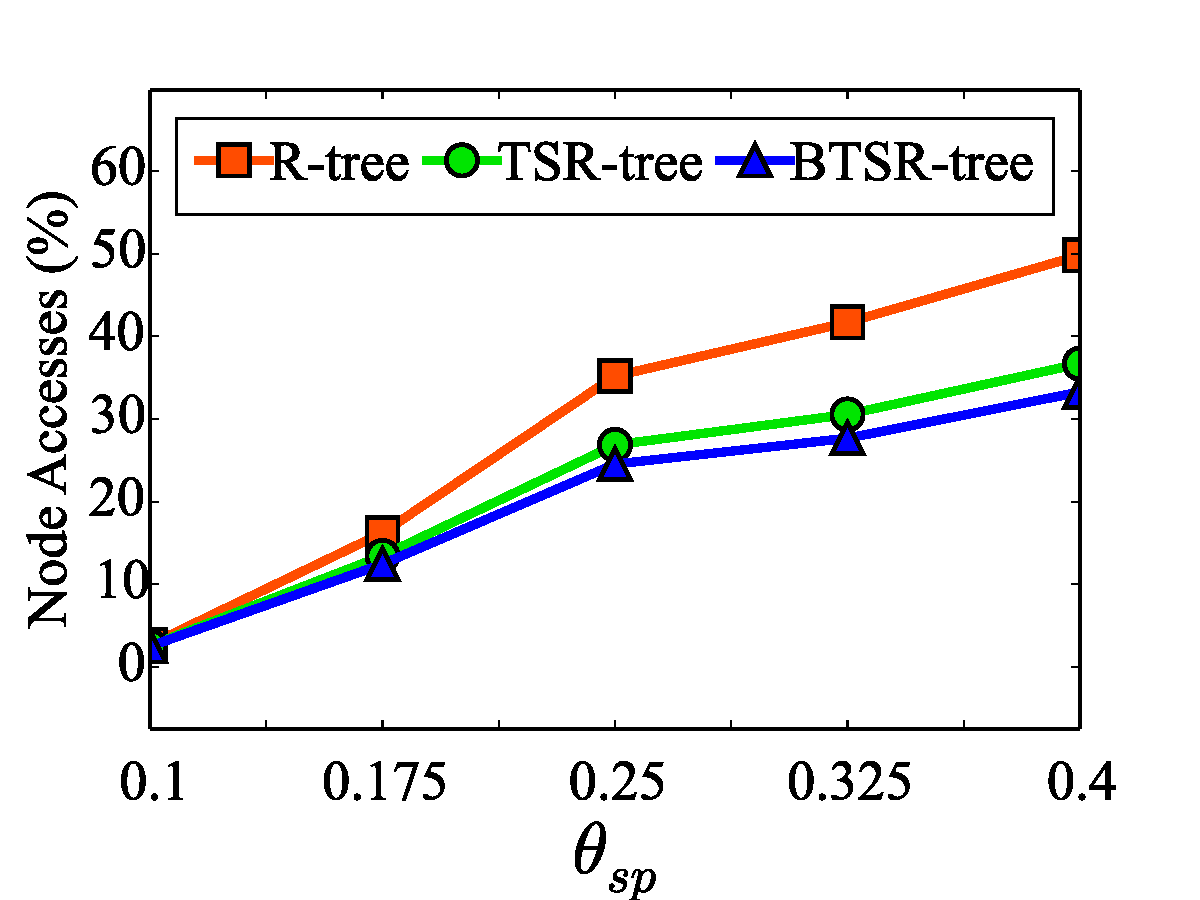
\includegraphics[width=0.45\textwidth]{figures/plots/flickr/qbk_theta_sp.pdf}\label{subfig:qbk_theta_sp_flickr}}
	\subfloat[Crime]{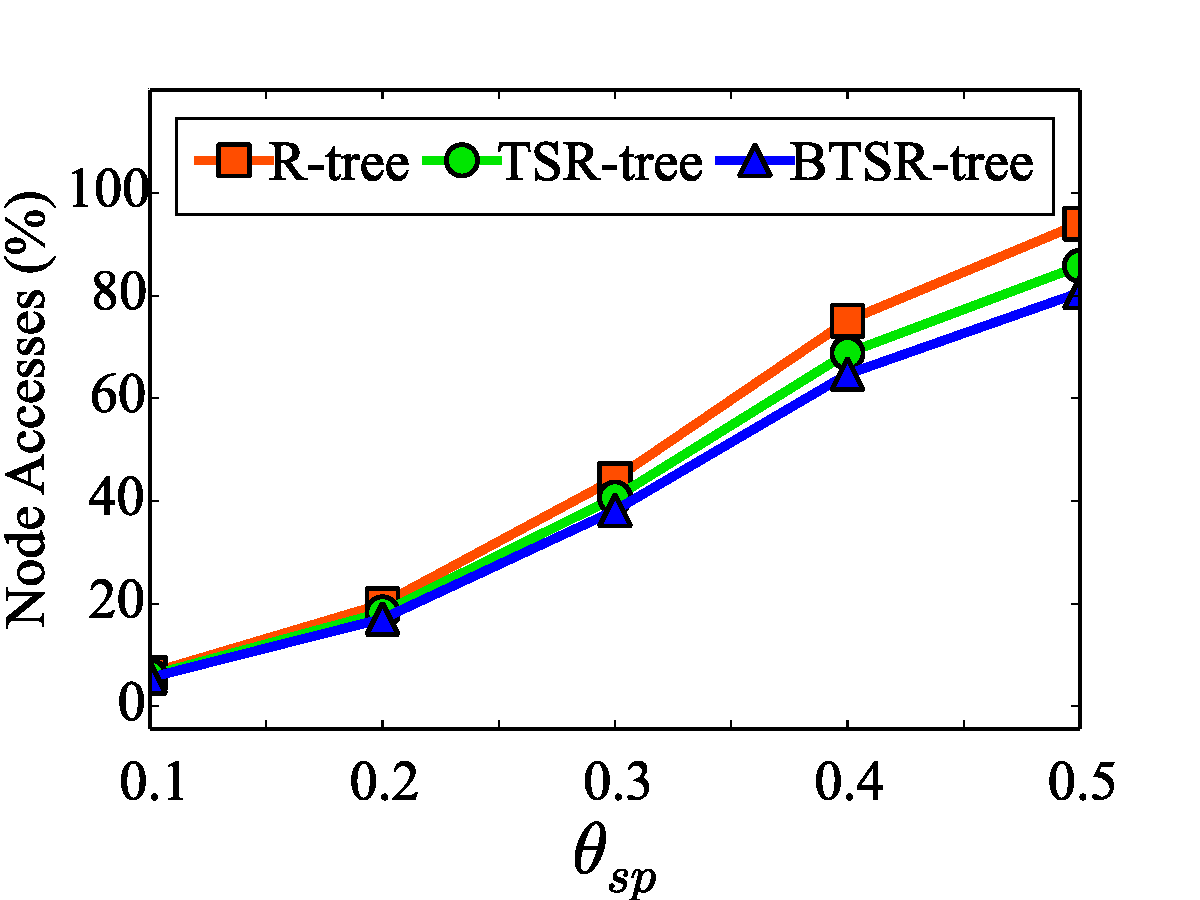
\includegraphics[width=0.45\textwidth]{figures/plots/crime/qbk_theta_sp.pdf}\label{subfig:qbk_theta_sp_crime}}
	\caption{Query $Q_{bk}(T_q, \theta_{sp}, k)$ with varying spatial distance threshold $\theta_{sp}$.}
	\label{fig:query_qbk_theta_sp}
\end{figure}

\paragraph{$Q_{hb}$ and $Q_{hk}$.} First, note that such hybrid queries cannot be possibly applied on the R-tree at all. Regarding the $Q_{hb}$ query, Figure \ref{fig:query_qhb_theta_h} plots performance for varying hybrid distance threshold ($\theta_{hb}$). The \btsr fares better than the \tsr in all cases. The effect is more intense with smaller $\theta_{hb}$ values, since the tighter bundles in the \btsr allow more effective pruning. For each dataset, divergence in performance between the two indices largely depends on variance among closely located time series. For instance, taxi dropoffs exhibit similar patterns locally, so the derived bounds also tend to be similar, diminishing the pruning power of both indices as shown in Figure \ref{subfig:qhb_theta_h_taxi}. Instead, when nearby time series have many diverse patterns, the \btsr becomes more effective by allocating them to distinct bundles and offering considerable performance gain as for the Water dataset (Figure~\ref{subfig:qhb_theta_h_water}).

\begin{figure}[!ht]
	\centering
	\subfloat[Water]{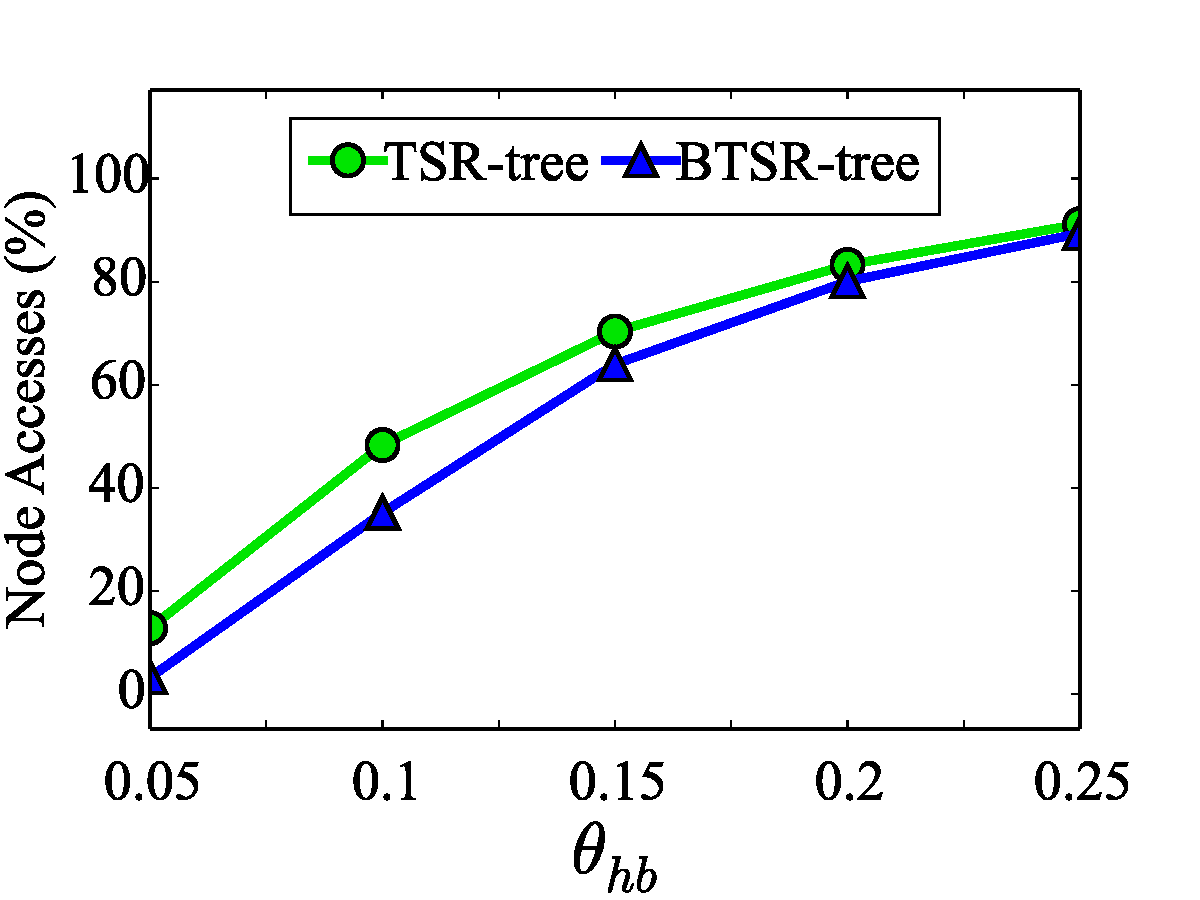
\includegraphics[width=0.45\textwidth]{figures/plots/water/qhb_theta_h.pdf}\label{subfig:qhb_theta_h_water}}
	\subfloat[Taxi]{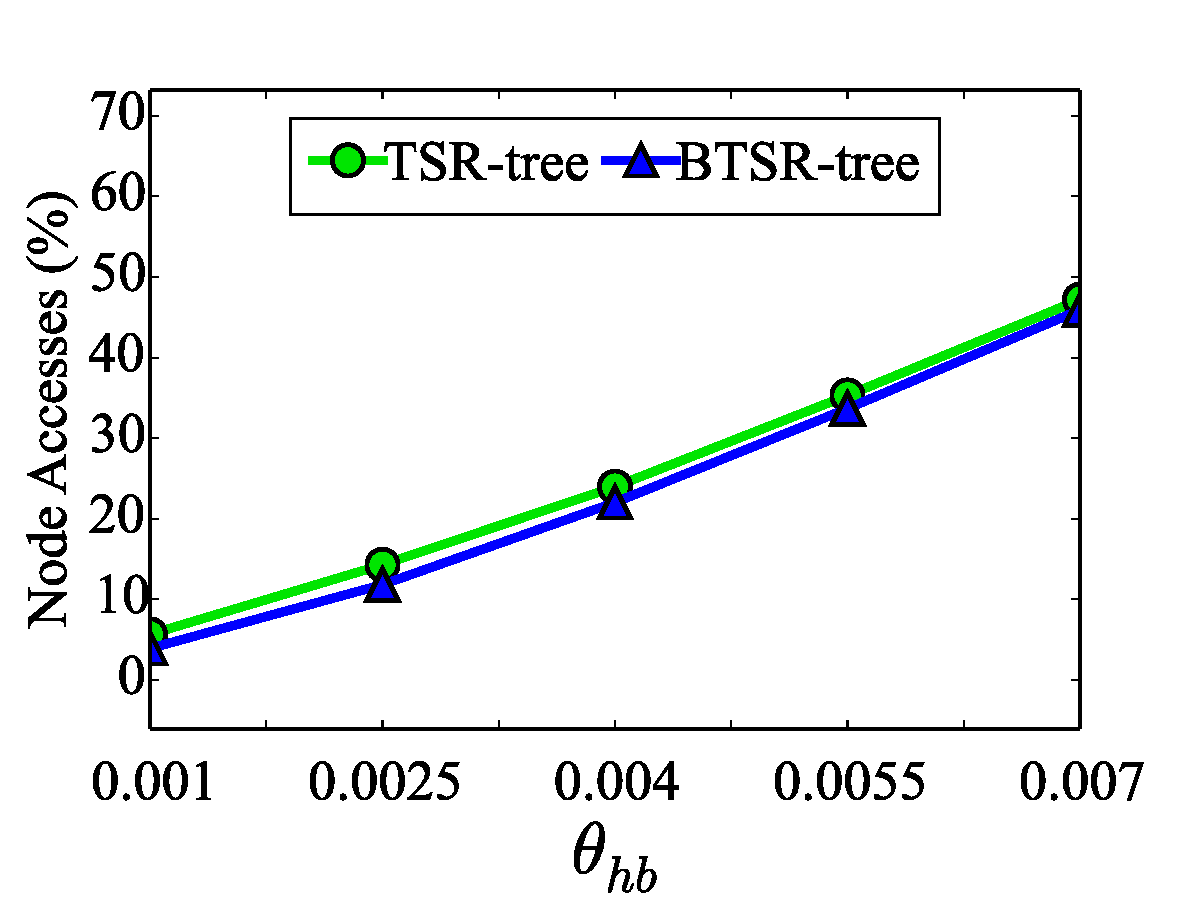
\includegraphics[width=0.45\textwidth]{figures/plots/taxi/qhb_theta_h.pdf}\label{subfig:qhb_theta_h_taxi}} \\
	\subfloat[Flickr]{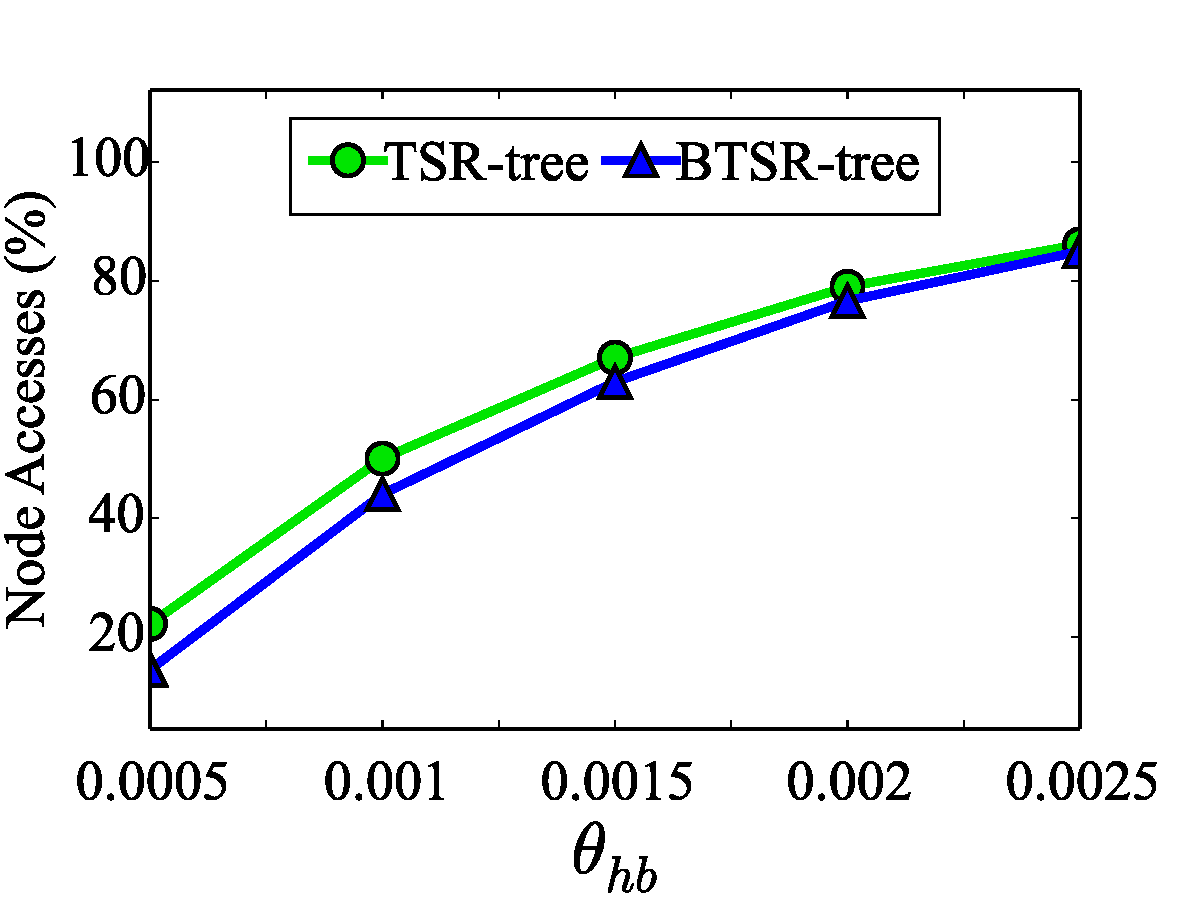
\includegraphics[width=0.45\textwidth]{figures/plots/flickr/qhb_theta_h.pdf}\label{subfig:qhb_theta_h_flickr}}
	\subfloat[Crime]{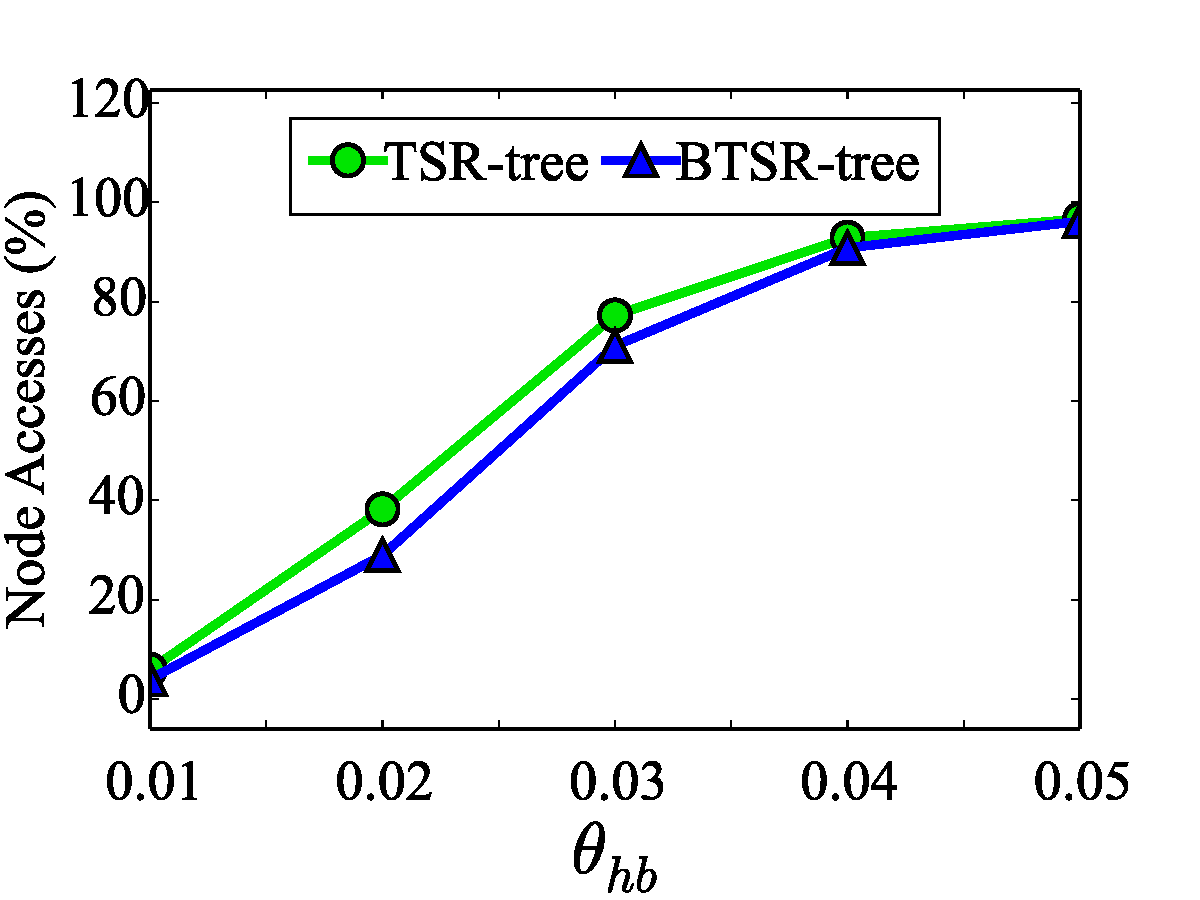
\includegraphics[width=0.45\textwidth]{figures/plots/crime/qhb_theta_h.pdf}\label{subfig:qhb_theta_h_crime}}
	\caption{Query $Q_{hb}(T_q, \theta_h, \gamma)$ with varying hybrid distance threshold $\theta_h$.}
	\label{fig:query_qhb_theta_h}
\end{figure}


Finally, Figure \ref{fig:query_qhk_k} depicts the performance of $Q_{hk}$ for varying number $k$ of results. \btsr always outperforms \tsr  with a margin of more than $10\%$ node accesses on average, again with the exception of the Taxi dataset (Figure \ref{subfig:qhk_k_taxi}), as mentioned before.

\begin{figure}[!ht]
	\centering
	\subfloat[Water]{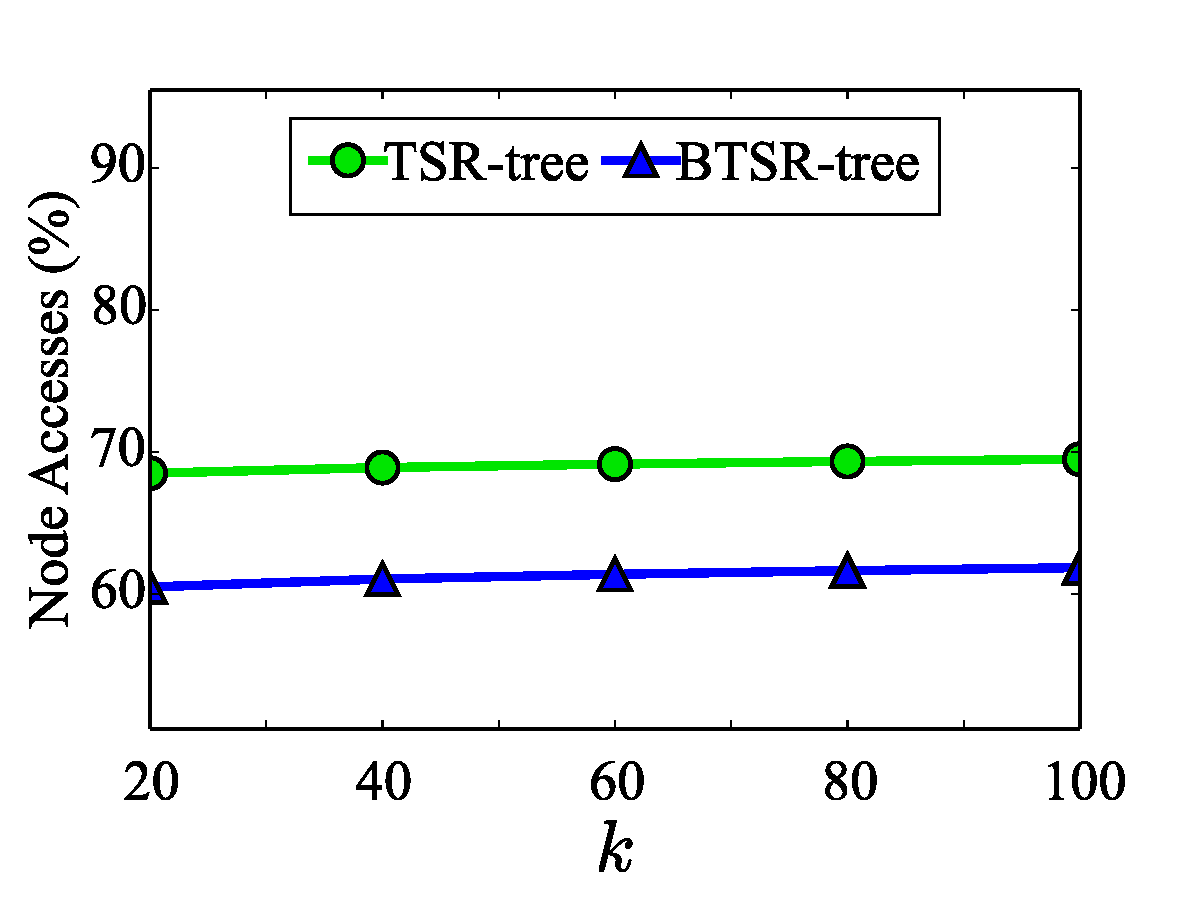
\includegraphics[width=0.45\textwidth]{figures/plots/water/qhk_k.pdf}\label{subfig:qhk_k_water}}
	\subfloat[Taxi]{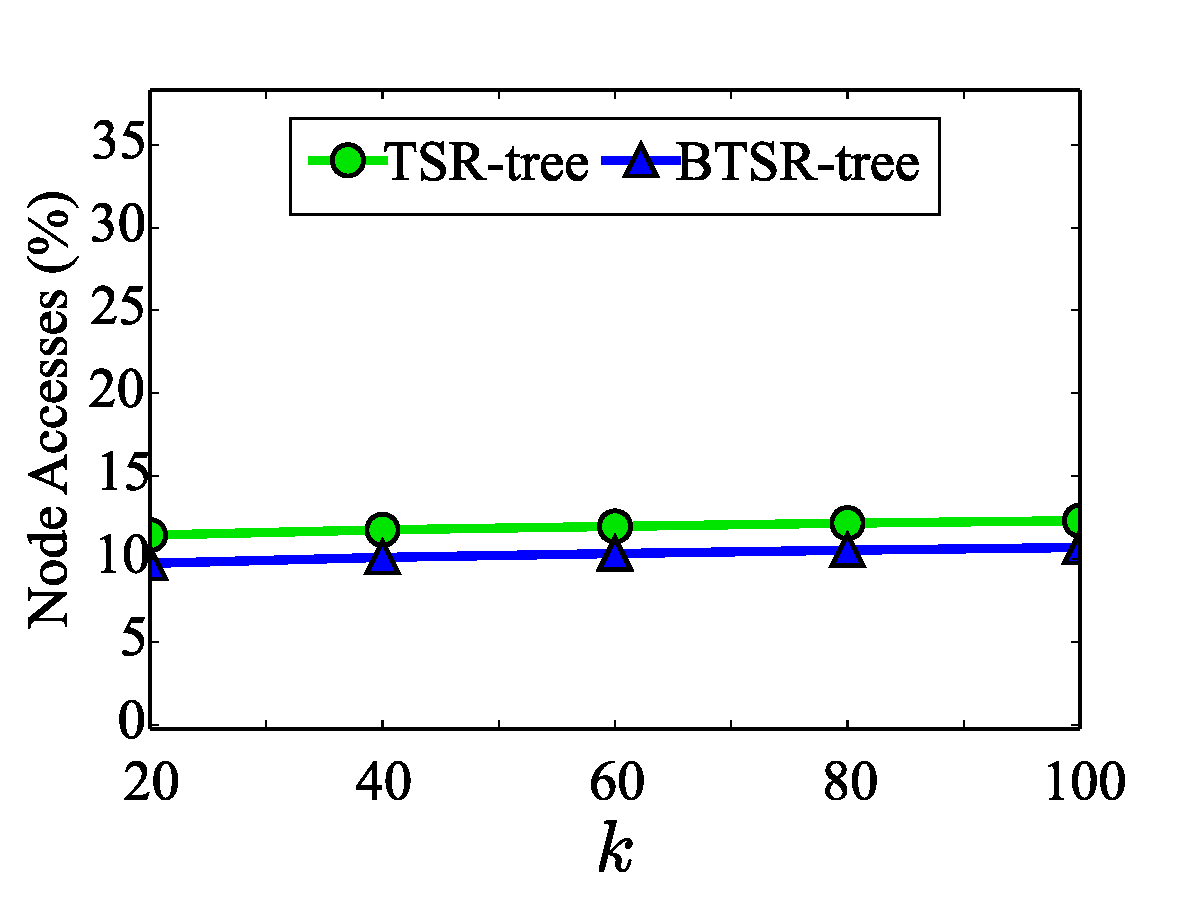
\includegraphics[width=0.45\textwidth]{figures/plots/taxi/qhk_k.pdf}\label{subfig:qhk_k_taxi}} \\
	\subfloat[Flickr]{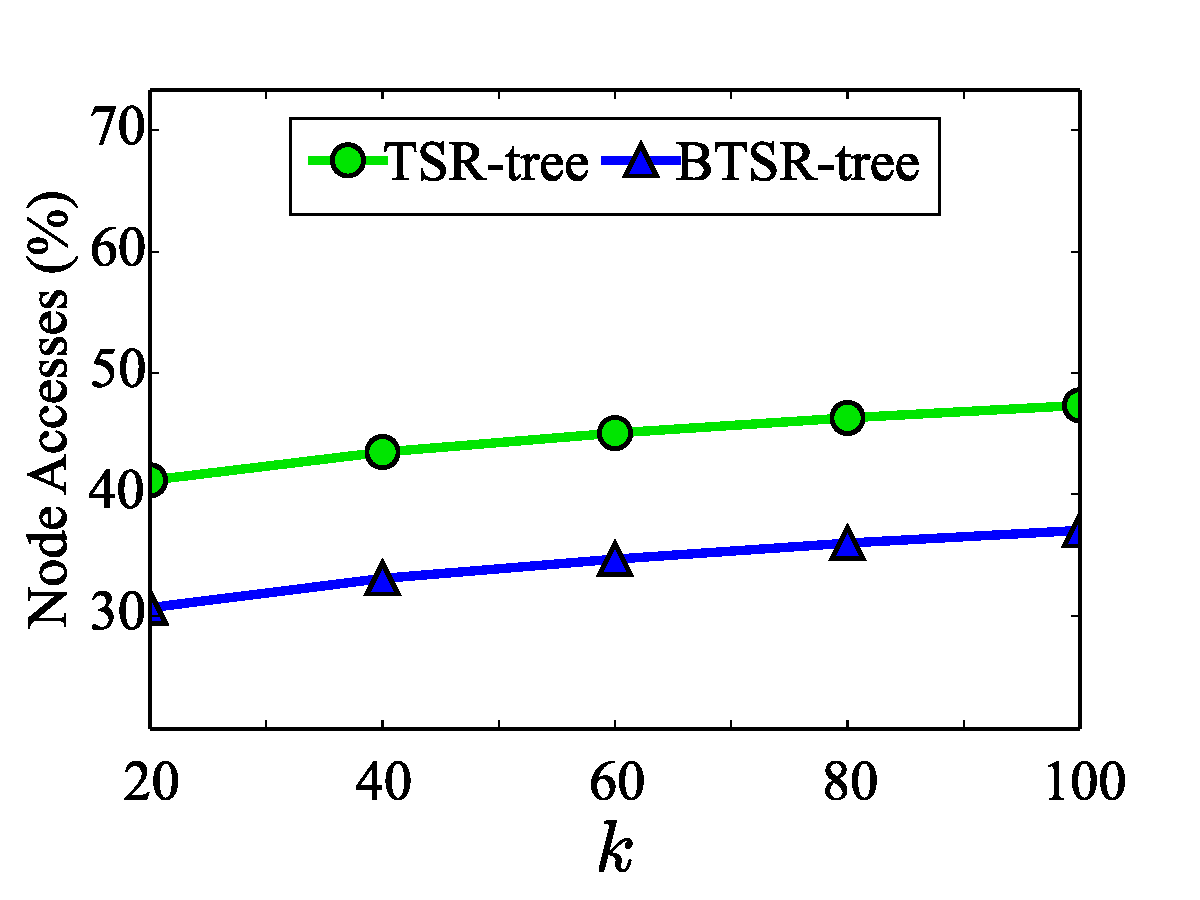
\includegraphics[width=0.45\textwidth]{figures/plots/flickr/qhk_k.pdf}\label{subfig:qhk_k_flickr}}
	\subfloat[Crime]{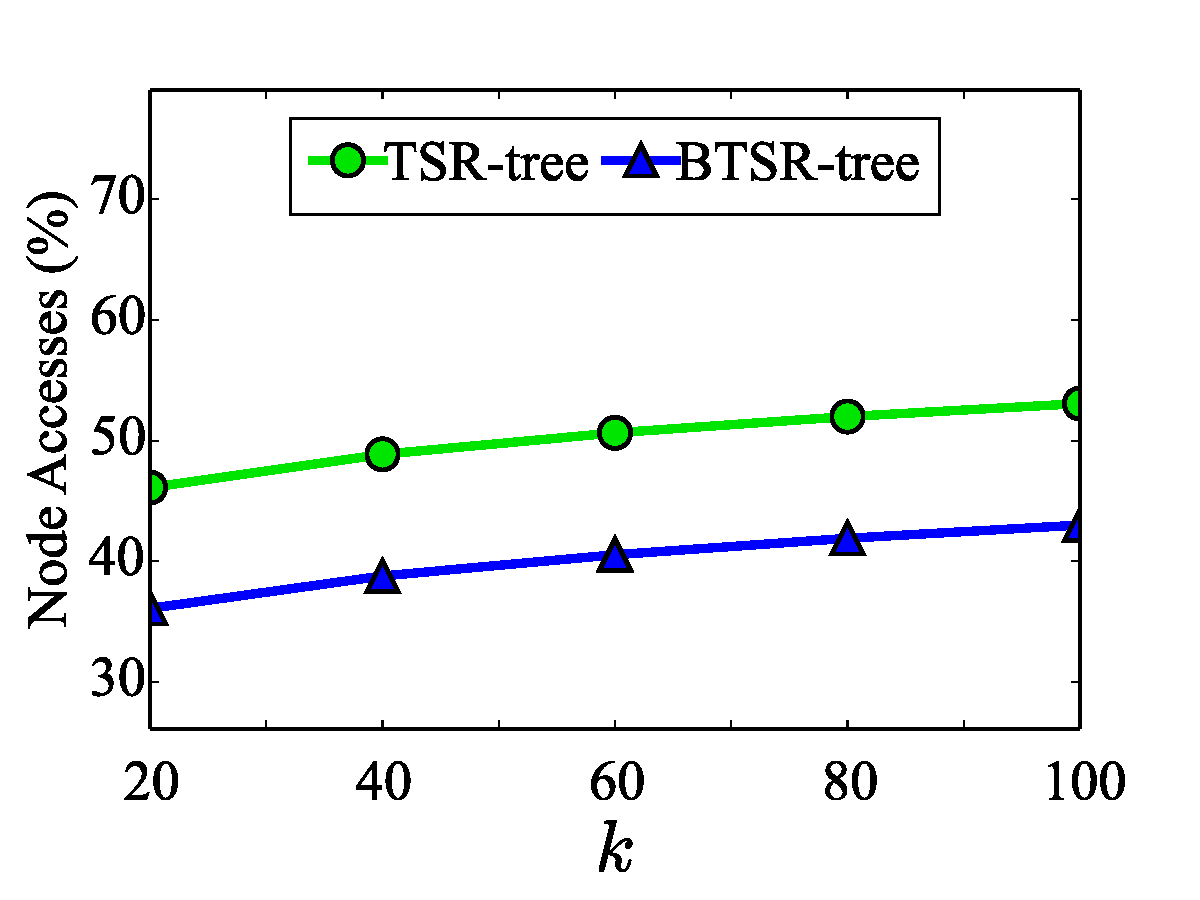
\includegraphics[width=0.45\textwidth]{figures/plots/crime/qhk_k.pdf}\label{subfig:qhk_k_crime}}
	\caption{Query $Q_{hk}(T_q, k, \gamma)$ with varying number $k$ of results.}
	\label{fig:query_qhk_k}
\end{figure}

\subsubsection{Centralized HSJ Results}
\label{subsec:centralized_results}

Figure \ref{exp:centralized} depicts performance for different parameter values and dataset sizes. The \isax-based algorithm performs significantly worse than the rest, mostly because each node comparison involves reconversion of the \isax symbols to the Euclidean space \cite{shieh2008kdd} and consequently, calculation of Euclidean distances over long sequences (up to 168 values in this data). \btsr is superior in all cases, as it is able to prune in both time series and spatial domains. As shown in Figure \ref{exp:EpsSPCentralized}, \btsr and \rtree-based methods perform similarly for smaller $\epsilon_{sp}$ values, as fewer candidates are found and need refinement in the time series domain. However, as the distance radius $\epsilon_{sp}$ is relaxed, \rtree search worsens significantly, while \btsr still copes well due to its hybrid pruning ability. \isax-based search is immune to different values of $\epsilon_{sp}$, as filtering with spatial distance is only involved at refinement. With varying $\epsilon_{ts}$ values (Figure \ref{exp:EpsTSCentralized}), \btsr and \rtree approaches have no fluctuations in performance, as $\epsilon_{sp}$ is fixed and refinement of candidates involves a similar cost in the time series domain. However, using \isax indexing is faster for lower $\epsilon_{ts}$ values and performance slowly degrades for larger $\epsilon_{ts}$, as more candidates become eligible. In terms of scalability (Figure \ref{exp:ScalabilityCentralized}), all algorithms are almost equally fast over small datasets. But, as dataset sizes grow, the \btsr approach scales better thanks to its hybrid pruning, although the number of matching pairs escalates. Indicatively, for 100K input data, we get 2K qualifying pairs; in the 500K dataset, we get 40K results. For input data sizes larger than 500K, all centralized methods fail to finish execution, issuing an out-of-memory error. This manifests the necessity of distributed processing schemes for similarity joins over larger datasets.

\begin{figure}[!ht]
 \centering
 \subfloat[Varying $\epsilon_{sp}$]{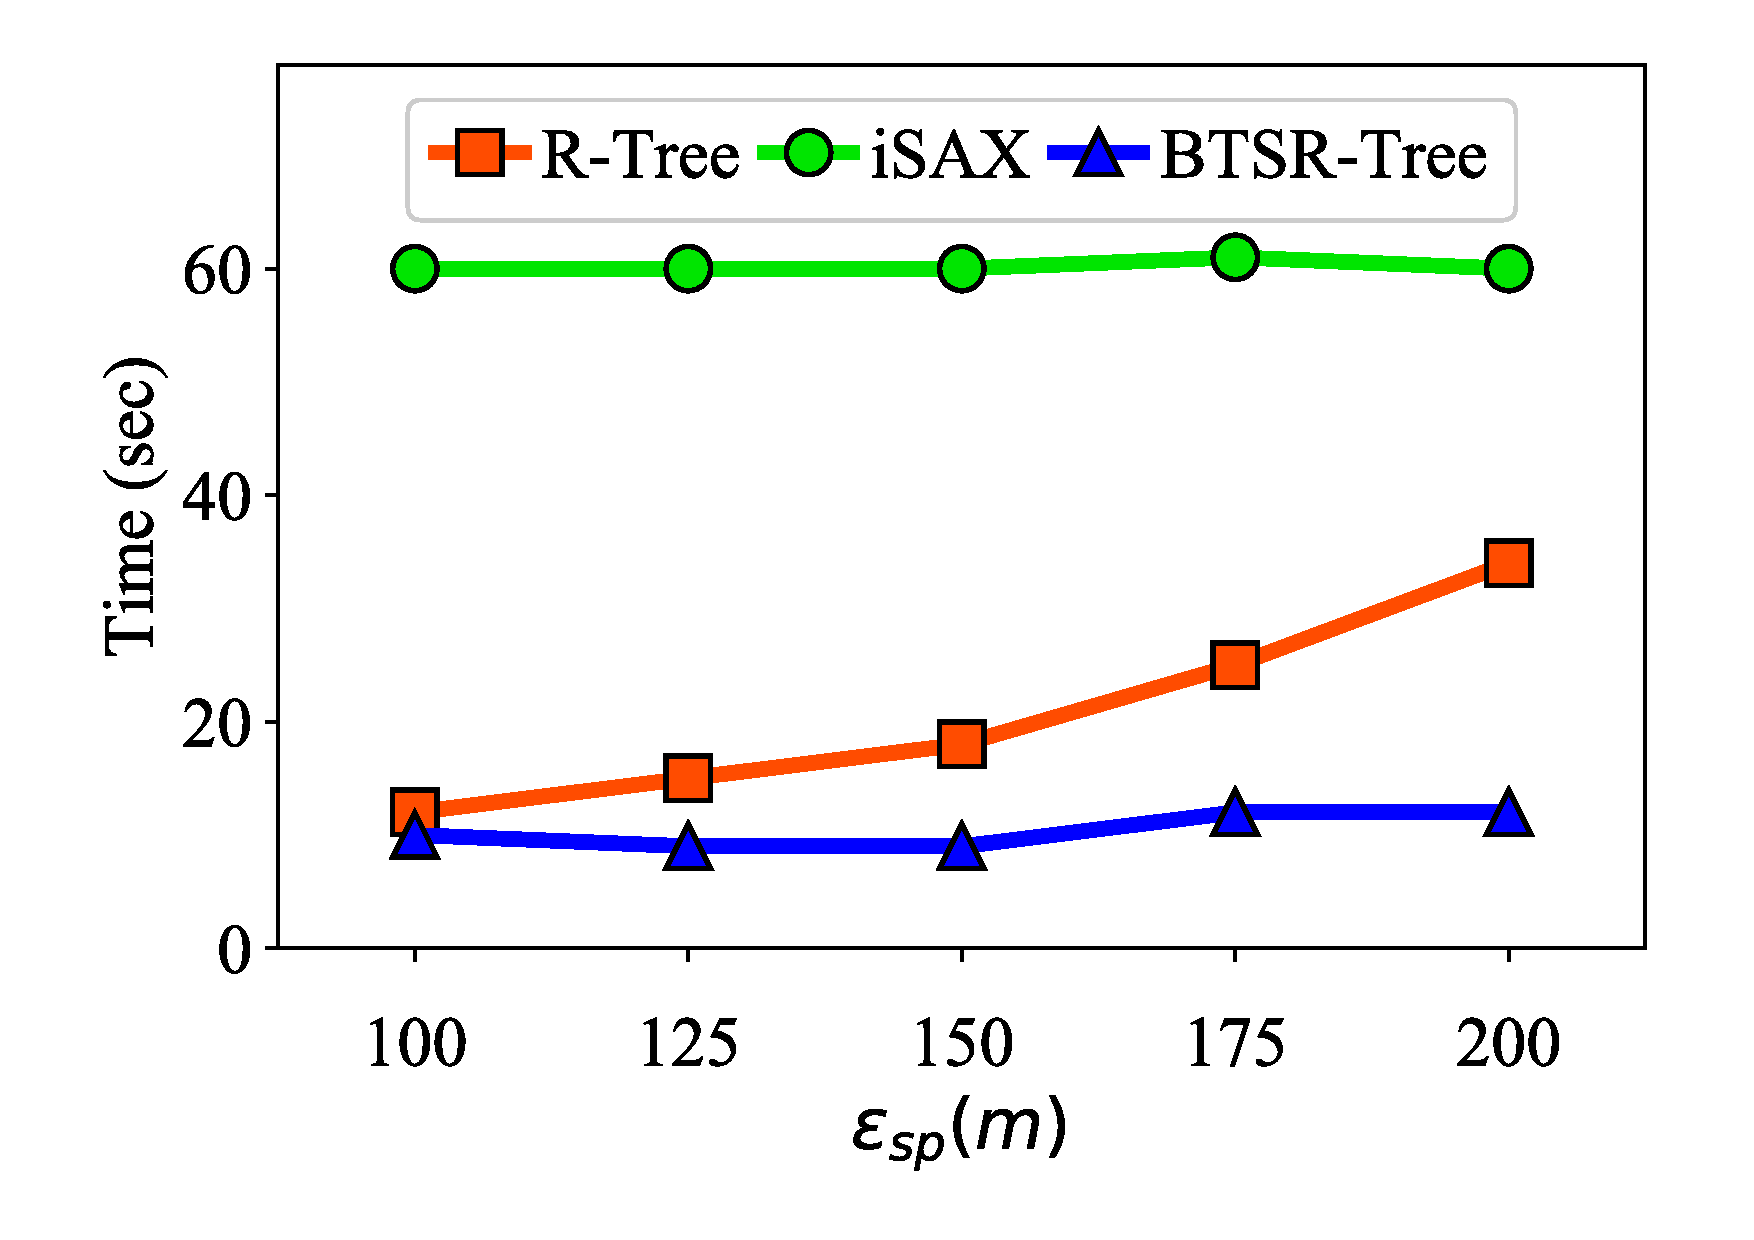
\includegraphics[trim=0.5cm 0.5cm 1cm 1cm, clip, width=0.325\textwidth]{figures/plots/EpsSPCentralized.pdf}\label{exp:EpsSPCentralized}}
 \subfloat[Varying $\epsilon_{ts}$]{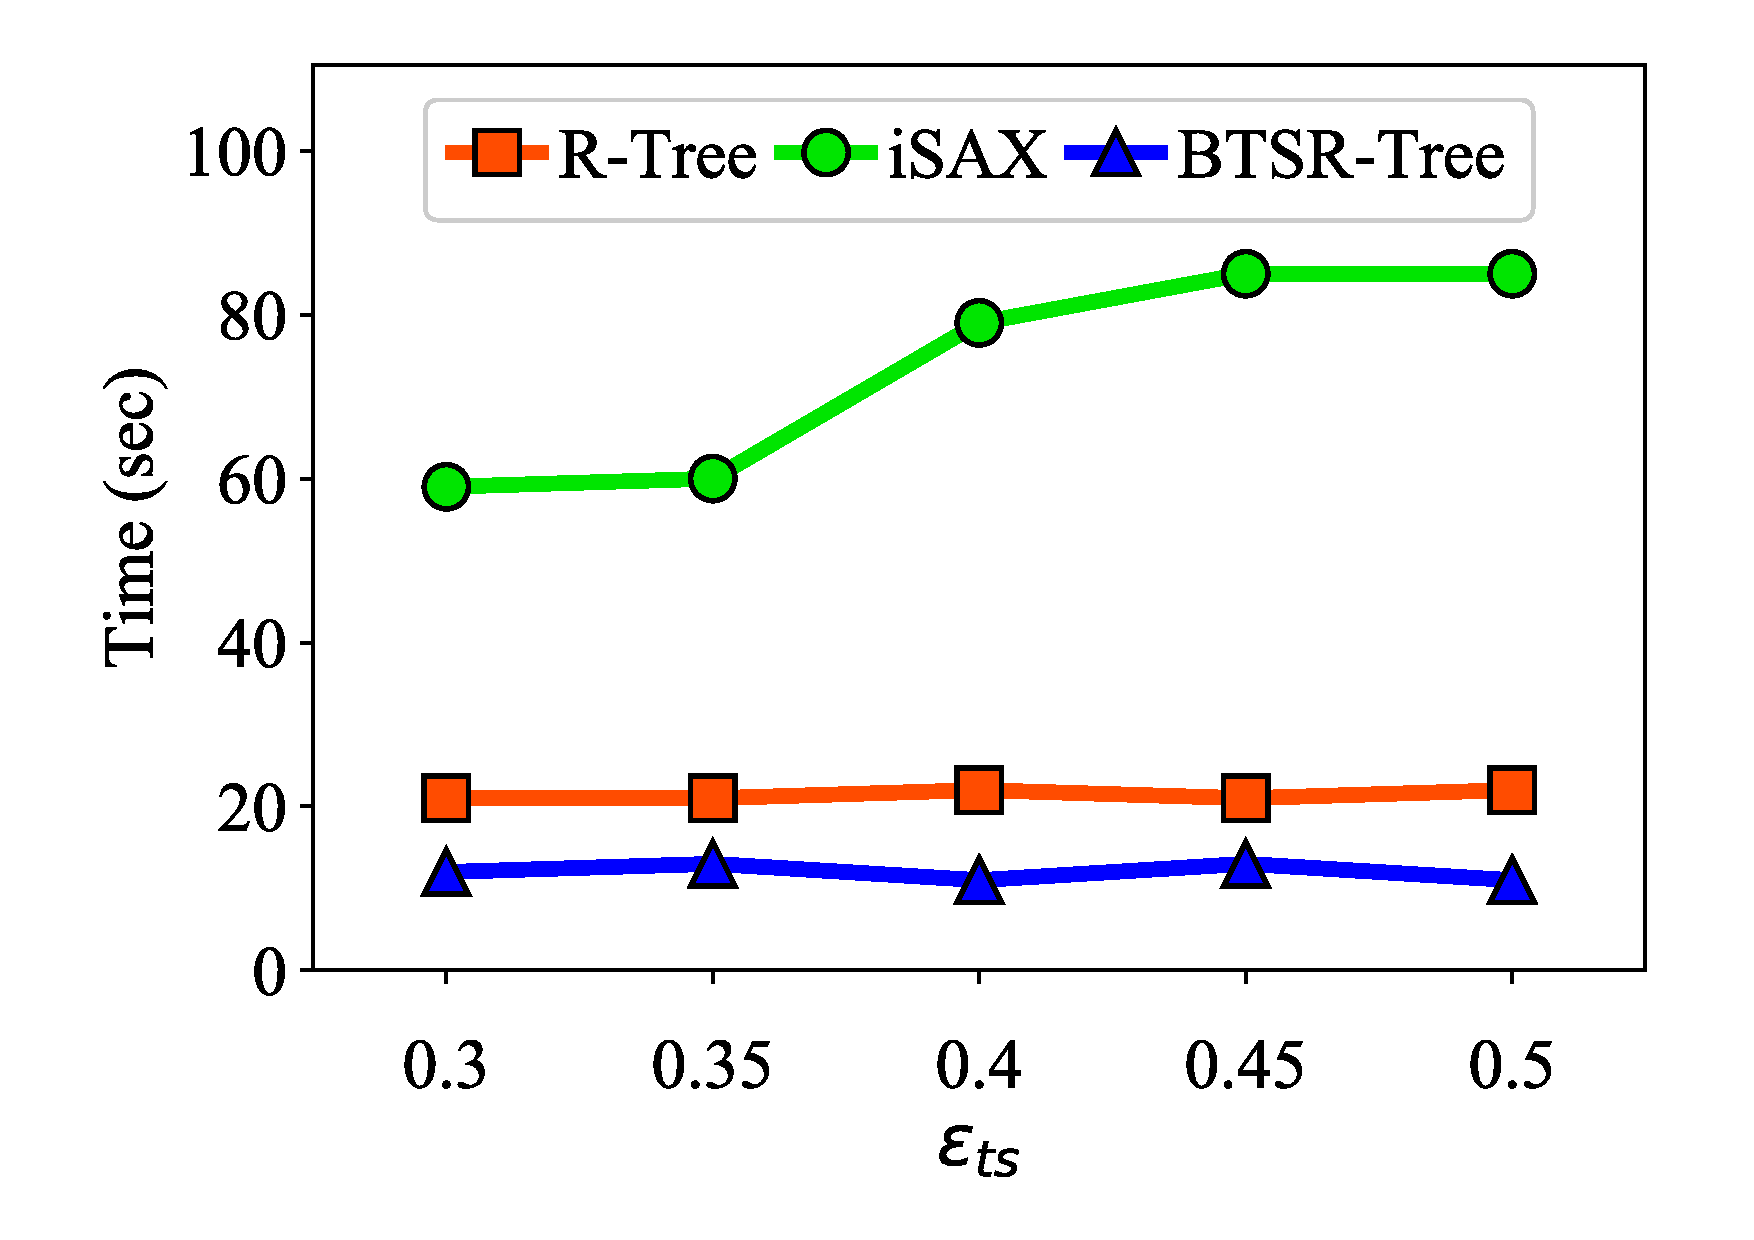
\includegraphics[trim=0.5cm 0.5cm 1cm 1cm, clip, width=0.325\textwidth]{figures/plots/EpsTSCentralized.pdf}\label{exp:EpsTSCentralized}}
 \subfloat[Scalability]{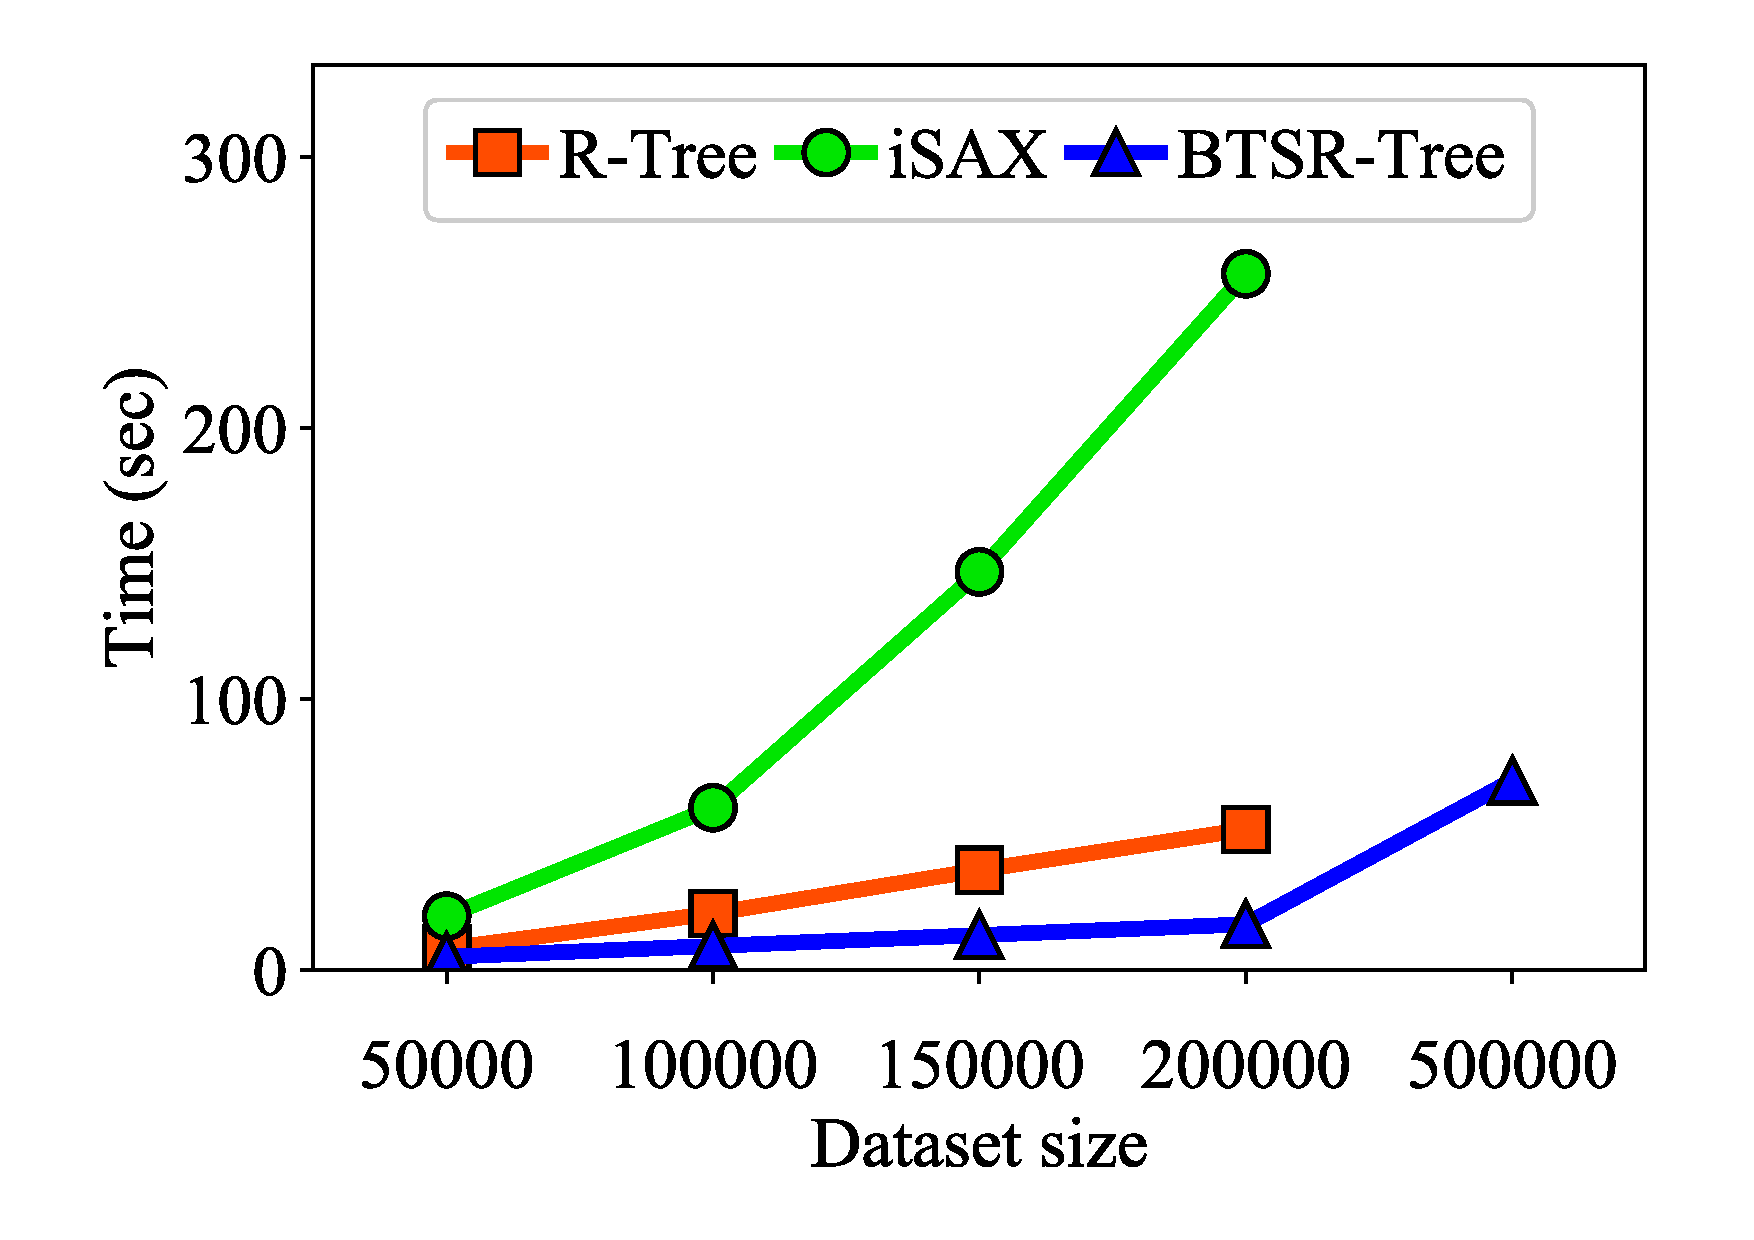
\includegraphics[trim=0.5cm 0.5cm 1cm 1cm, clip, width=0.325\textwidth]{figures/plots/ScalabilityCentralized.pdf}\label{exp:ScalabilityCentralized}}
 \caption{Processing cost for {\em centralized} execution of similarity join queries employing different indices.}
 \label{exp:centralized}
\end{figure}

\subsubsection{Distributed HSJ Results}
\label{subsec:distributed_results}

First, we compare \base (using R-trees for local indexing) with its \opt variant (employing {\btsr}s) for varying $\epsilon_{sp}$ values. It is apparent from Figure \ref{exp:EpsSPDist} that query response times for the \base method are increasing, since the underlying {\rtree}s fare worse for larger distance radii. With larger $\epsilon_{sp}$ values, more raw data has to be shuffled between workers during the cross-partition checks, as the size of bands and boxes involved gets bigger and covers more candidate geolocated time series. Concerning exactly this shuffling overhead, Figure~\ref{exp:EpsSPDistCommunication} reveals that this is indeed lower in the \opt variant, which explains its processing cost advantage. Finally, Figure \ref{exp:EpsSPDistResults} illustrates the number of results produced from the two stages; first locally in each partition, and then after cross-partition checks in bands and boxes. As distance constraint $\epsilon_{sp}$ gets more relaxed, more pairs qualify as answers. For smaller $\epsilon_{sp}$, the majority of results come locally from each partition. But as $\epsilon_{sp}$ is relaxed, many more pairs are found in neighboring partitions, as bands and boxes also become larger and increase their share in qualifying results much more.

\begin{figure}[!ht]
 \centering
 \subfloat[Query response time]{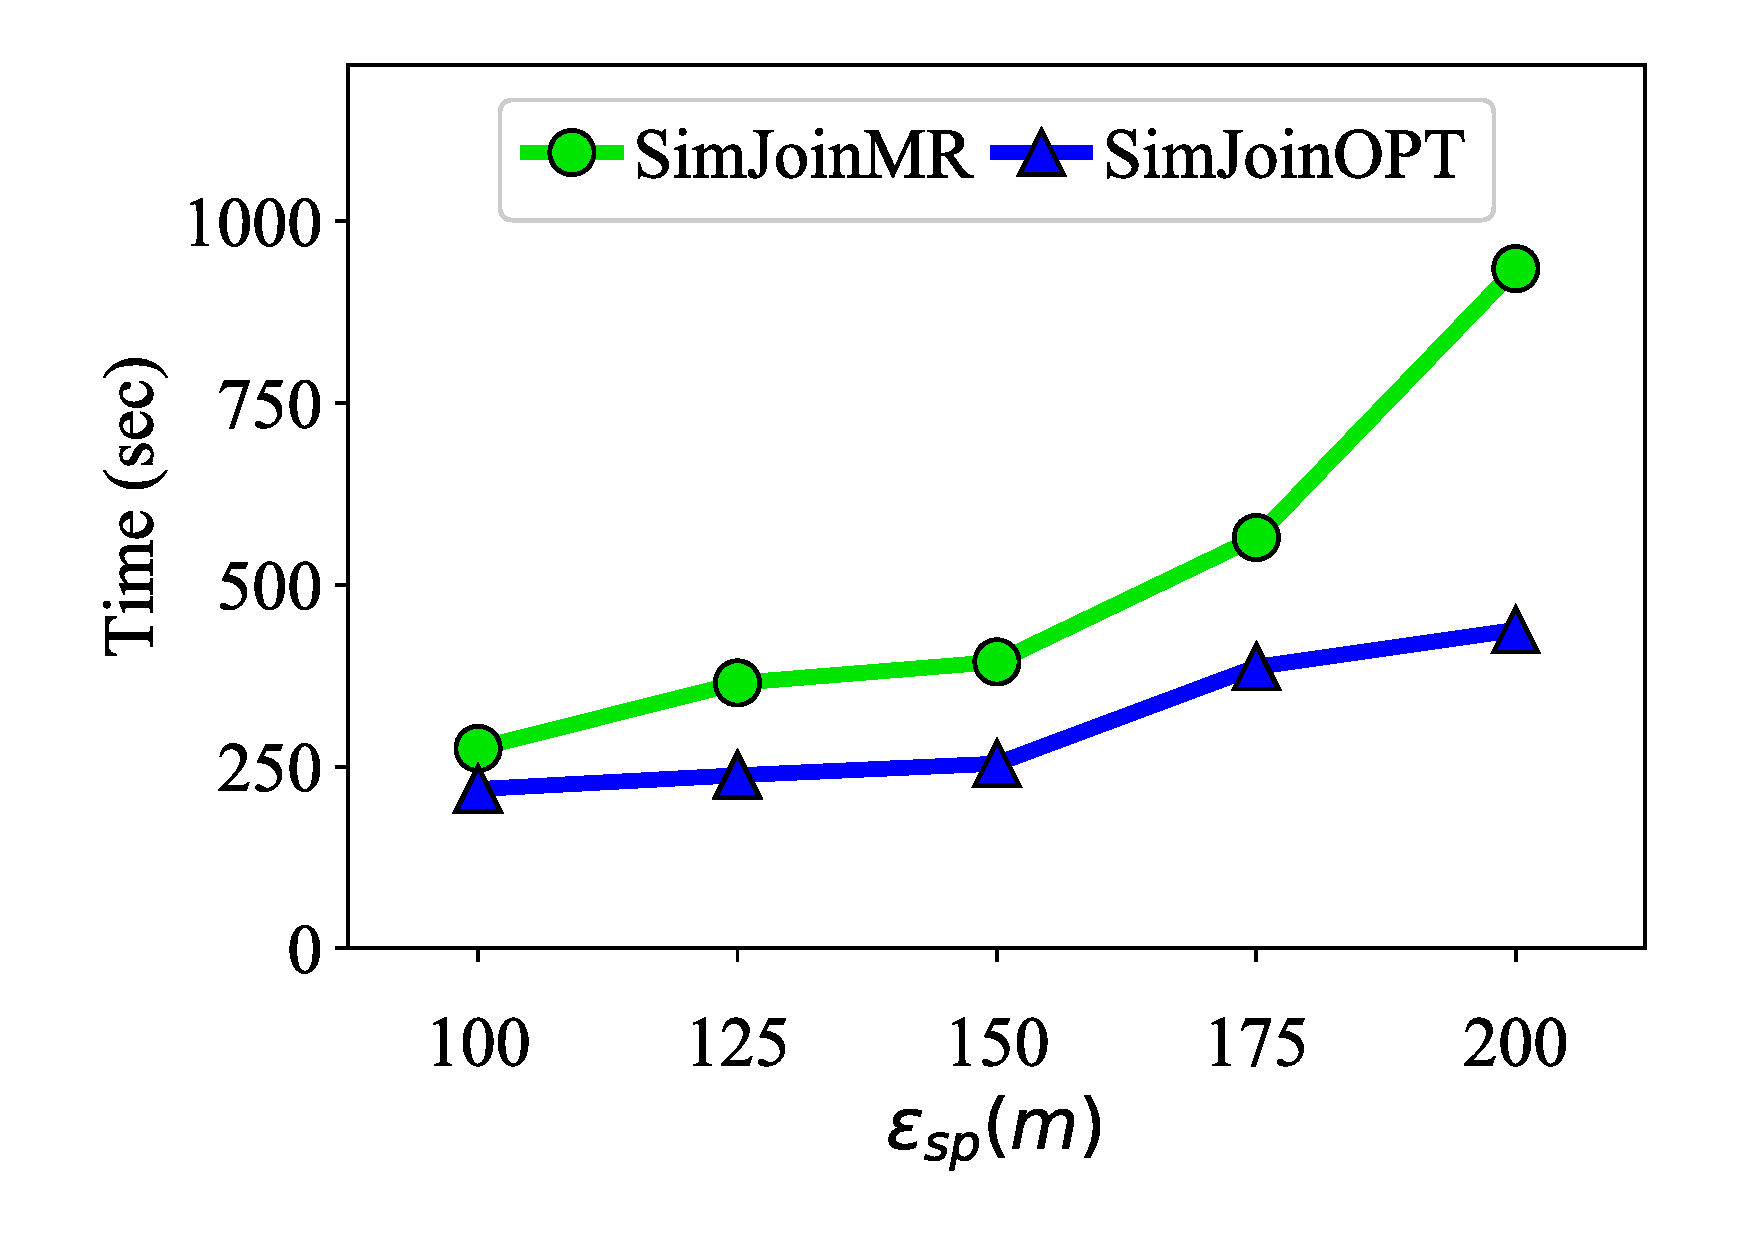
\includegraphics[trim=0.5cm 0.5cm 1cm 1cm, clip, width=0.325\textwidth]{figures/plots/EpsSPDist.pdf}\label{exp:EpsSPDist}}
 \subfloat[Geolocated time series shuffled]{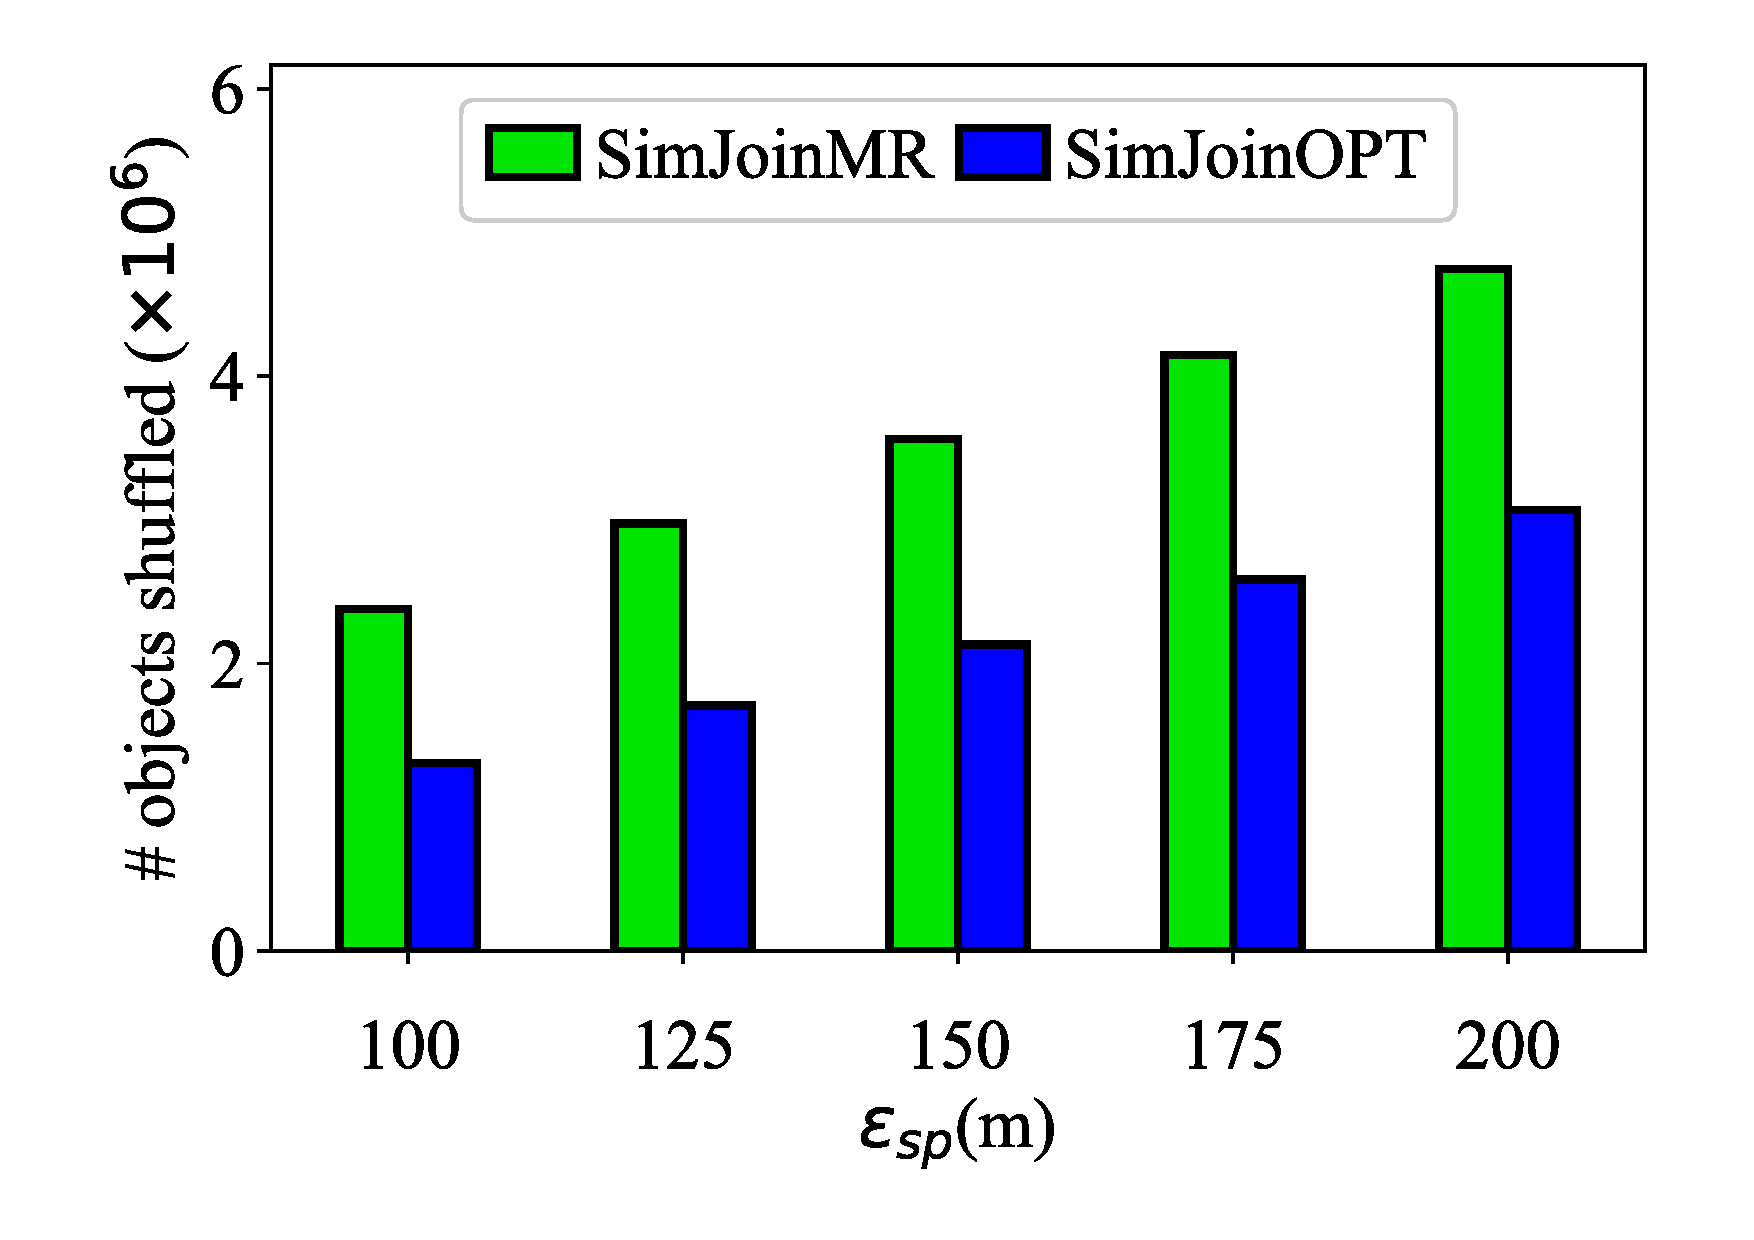
\includegraphics[trim=0.5cm 0.5cm 1cm 1cm, clip, width=0.325\textwidth]{figures/plots/EpsSPDistCommunication.pdf}\label{exp:EpsSPDistCommunication}}
 \subfloat[Query results per phase]{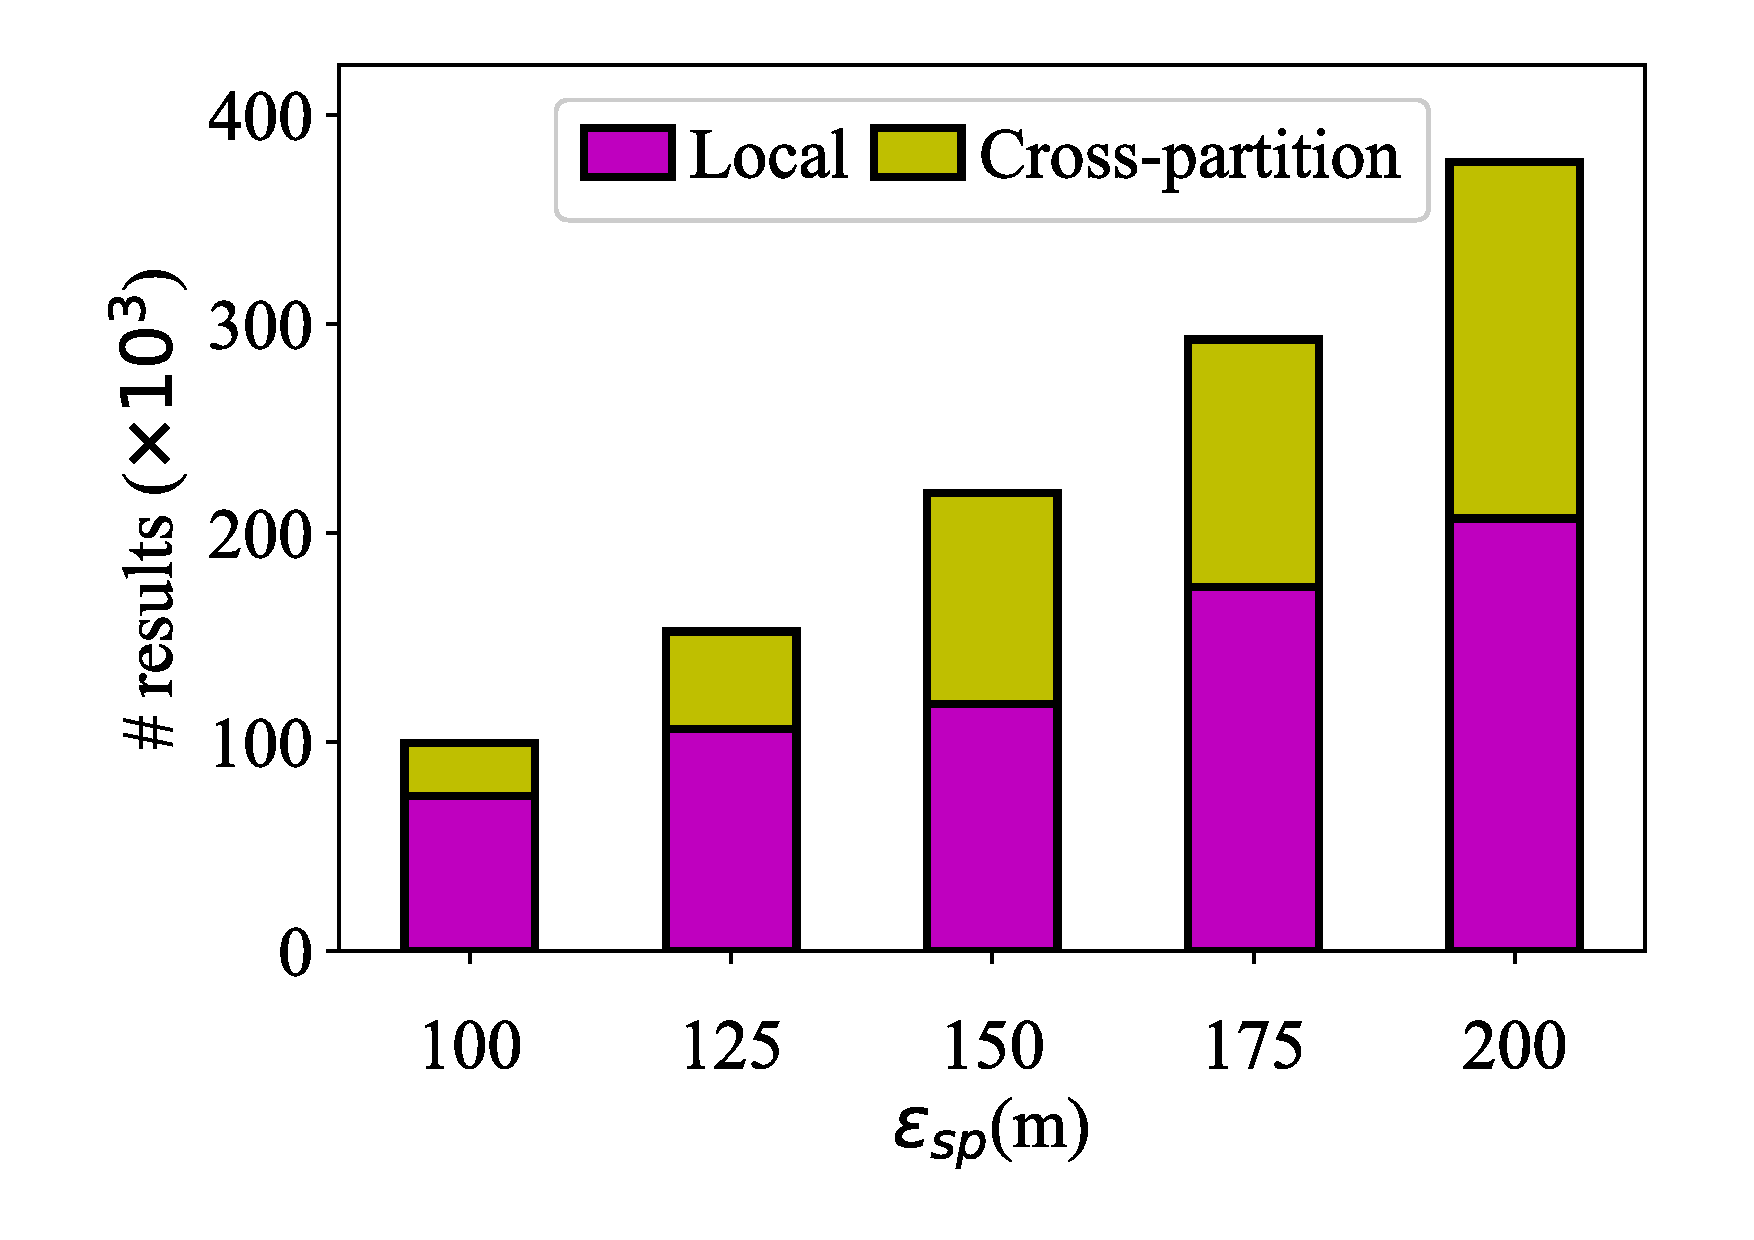
\includegraphics[trim=0.3cm 0.5cm 1.2cm 1cm, clip, width=0.325\textwidth]{figures/plots/EpsSPDistResults.pdf}\label{exp:EpsSPDistResults}}
 \caption{Performance results for the {\em distributed} methods with varying $\epsilon_{sp}$.}
 \label{exp:distr_EpsSP}
\end{figure}

With regard to increasing $\epsilon_{ts}$ values, observe in Figure \ref{exp:EpsTSDist} that method \base is consistently worse than \opt, basically due to the different pruning power of their respective indices. The former relies on R-trees, which have no effect with varying $\epsilon_{ts}$; in contrast, {\btsr}s employed by \opt can effectively filter candidates also in the time series domain. With a more relaxed $\epsilon_{ts}$, more results qualify, hence the linear increase in processing cost. Regarding the data shuffling overhead, this is practically stable for each method irrespective of the $\epsilon_{ts}$ constraint (Figure \ref{exp:EpsTSDistCommunication}). In \base, selection of geolocated time series that should be transmitted is solely based on their spatial containment in the respective bands and corner-wise boxes. But \opt avoids many irrelevant transfers, as it also uses filtering with $\epsilon_{ts}$; the amount of dispatched geolocated time series is only slightly increasing with $\epsilon_{ts}$. Regarding the number of generated results, Figure \ref{exp:EpsTSDistResults} reveals a rather steep increase for small variations of $\epsilon_{ts}$, which indicates that most time series are clustered within a small range of $\epsilon_{ts}$ deviations. As original data concern water consumption, this explains such highly correlated behavior, especially among neighboring households; of course, this pattern is replicated in the synthetic data as well. The percentage of results from cross-partition checks in each full answer is similar across various $\epsilon_{ts}$ values, as distance $\epsilon_{sp}$ is fixed and so are the respective bands and boxes involved in this phase.

\begin{figure}[!ht]
 \centering
 \subfloat[Query response time]{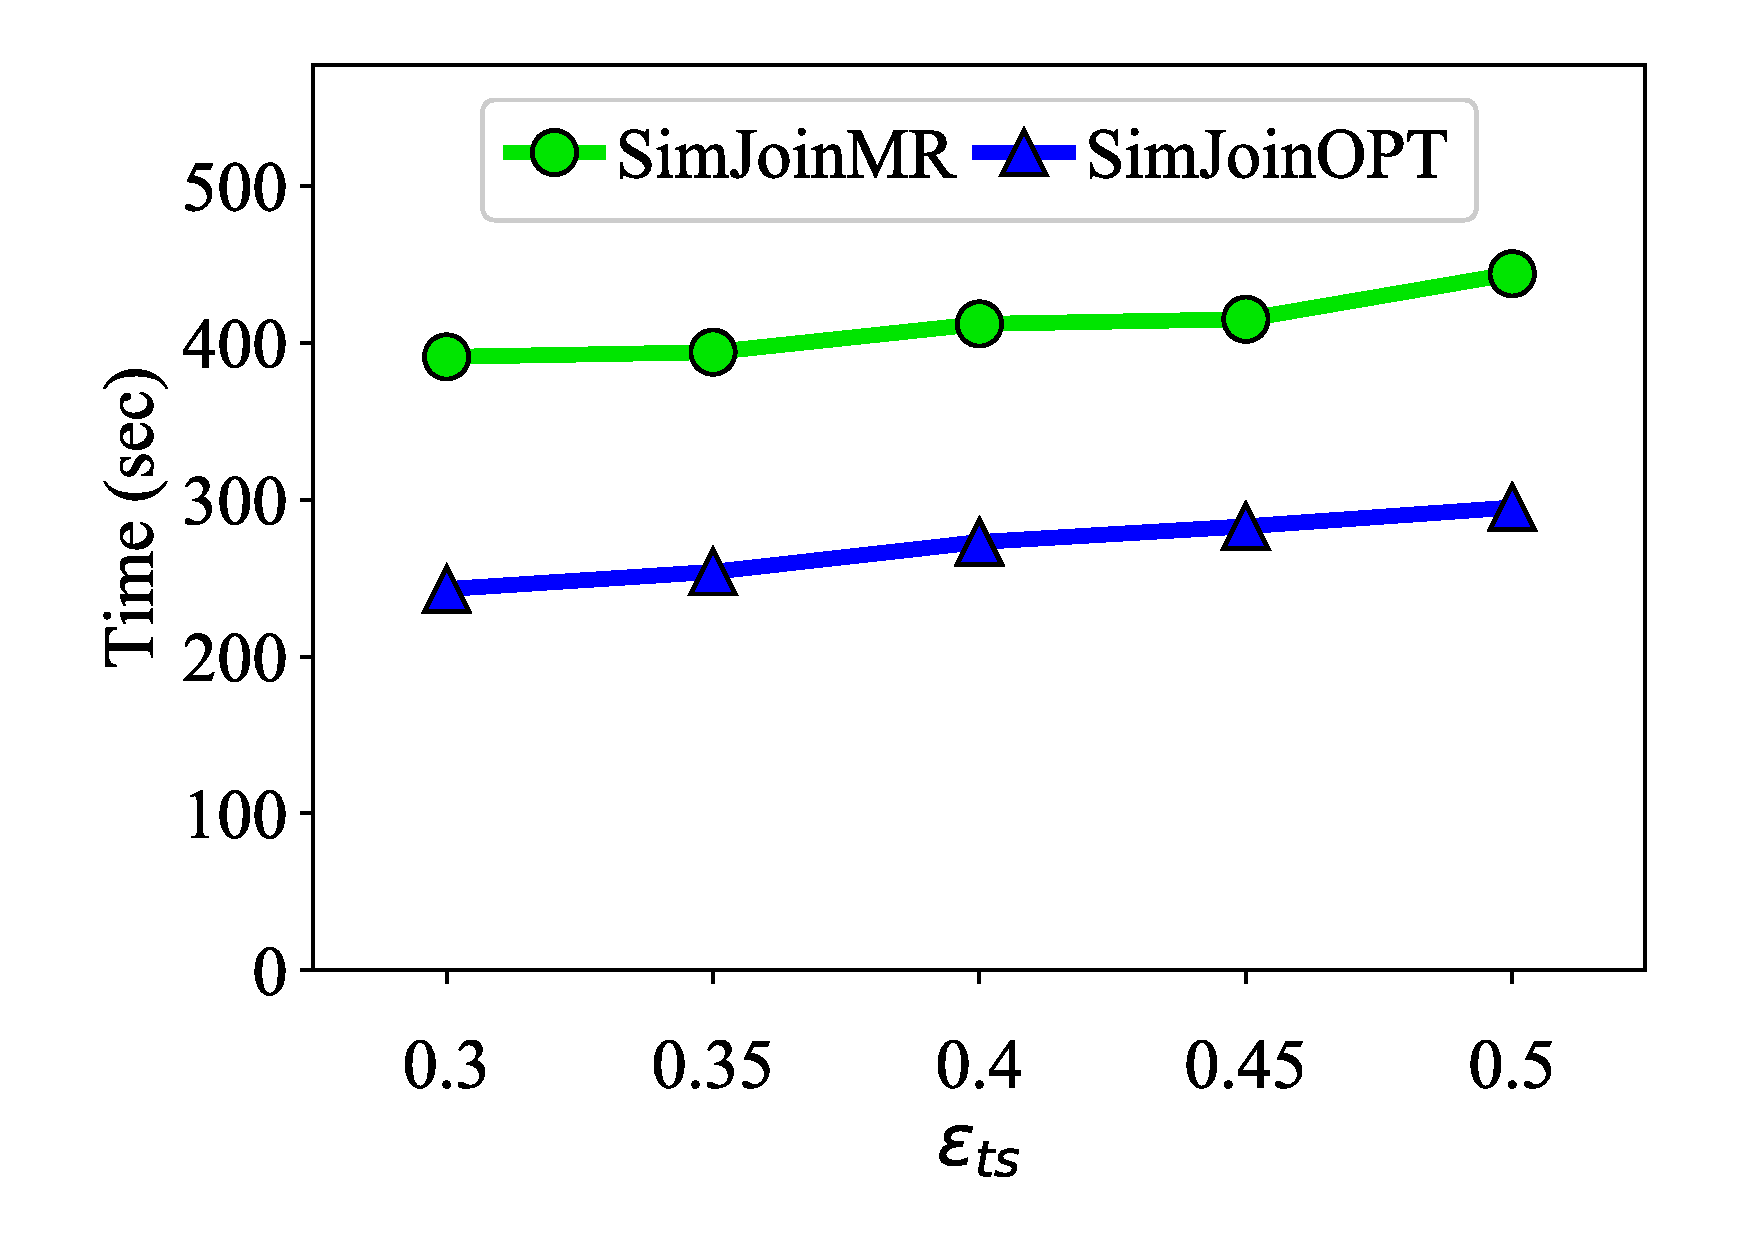
\includegraphics[trim=0.5cm 0.5cm 1cm 1cm, clip, width=0.325\textwidth]{figures/plots/EpsTSDist.pdf}\label{exp:EpsTSDist}}
 \subfloat[Geolocated time series shuffled]
 {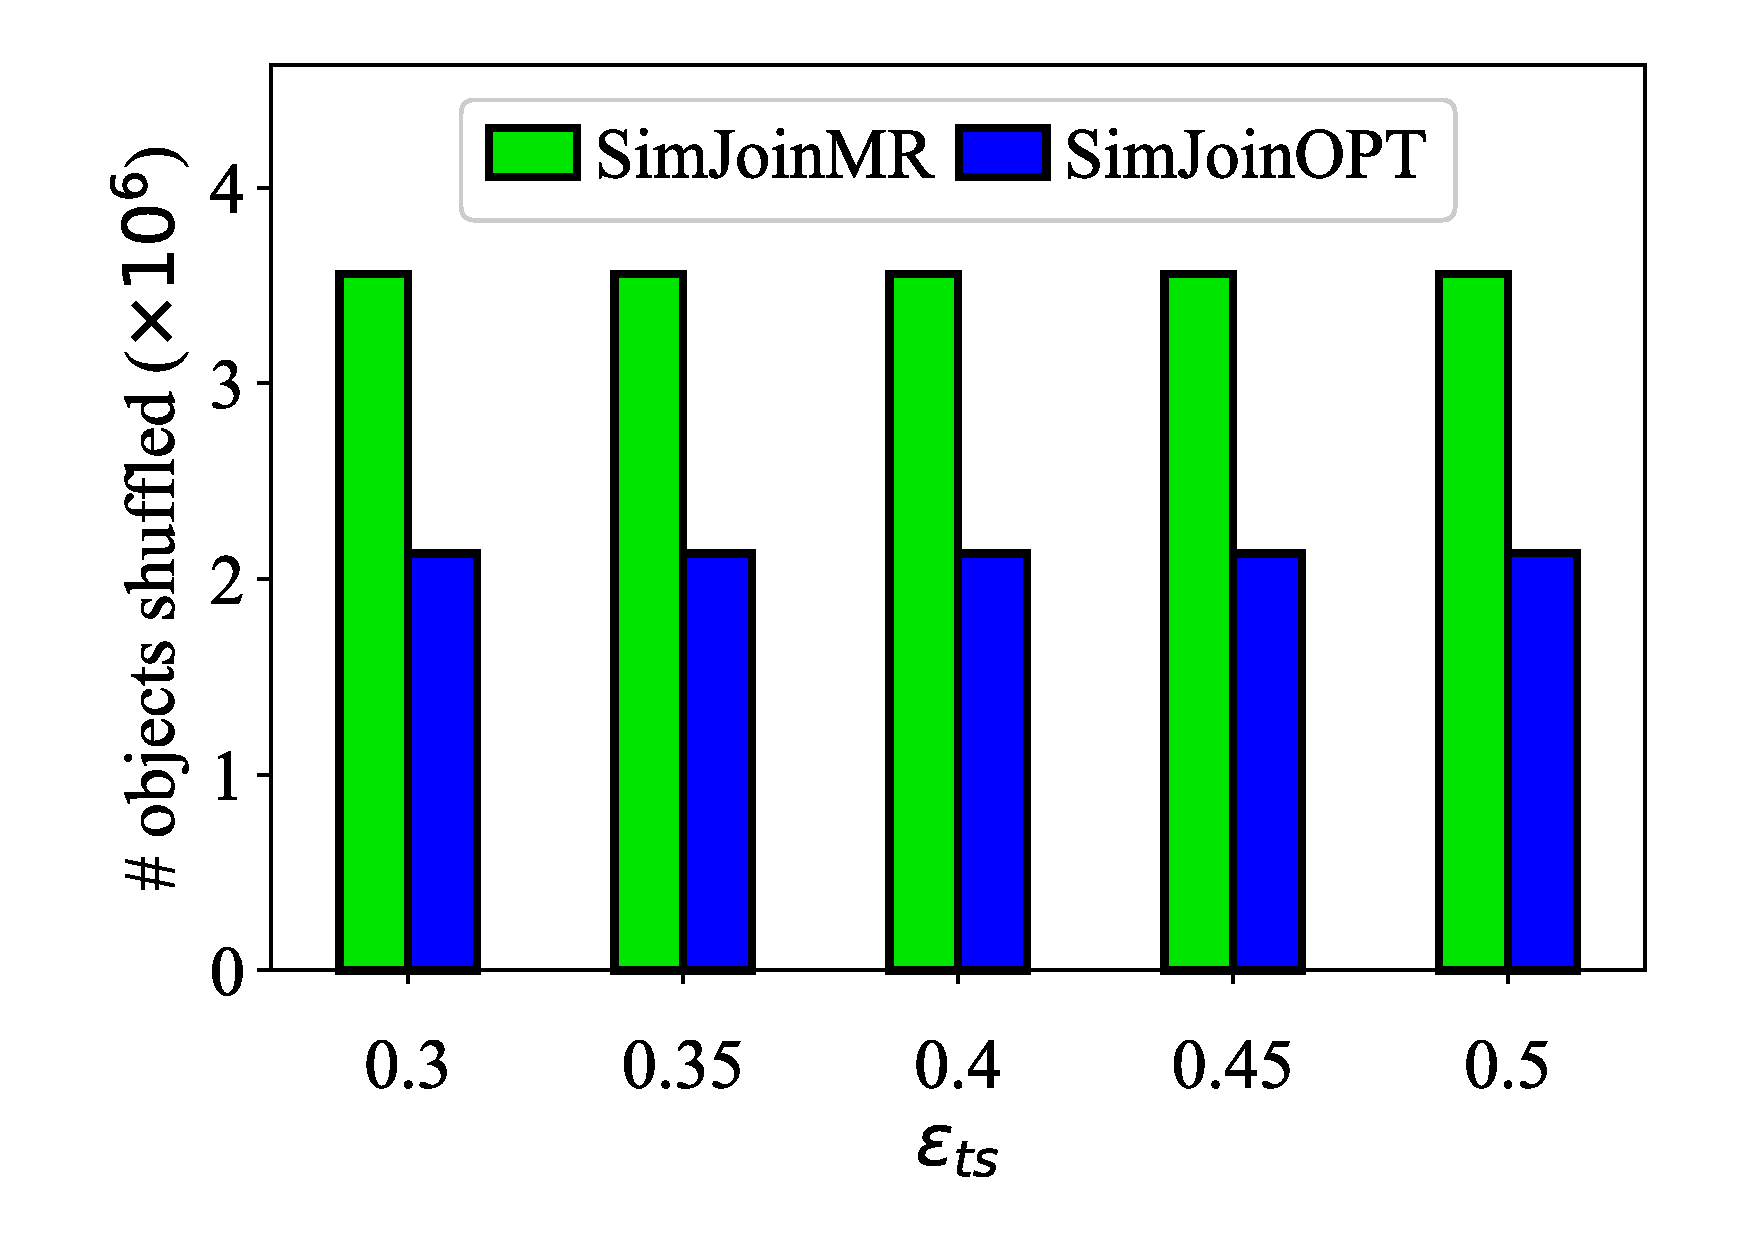
\includegraphics[trim=0.5cm 0.5cm 1cm 1cm, clip, width=0.325\textwidth]{figures/plots/EpsTSDistCommunication.pdf}\label{exp:EpsTSDistCommunication}}
 \subfloat[Query results per phase]{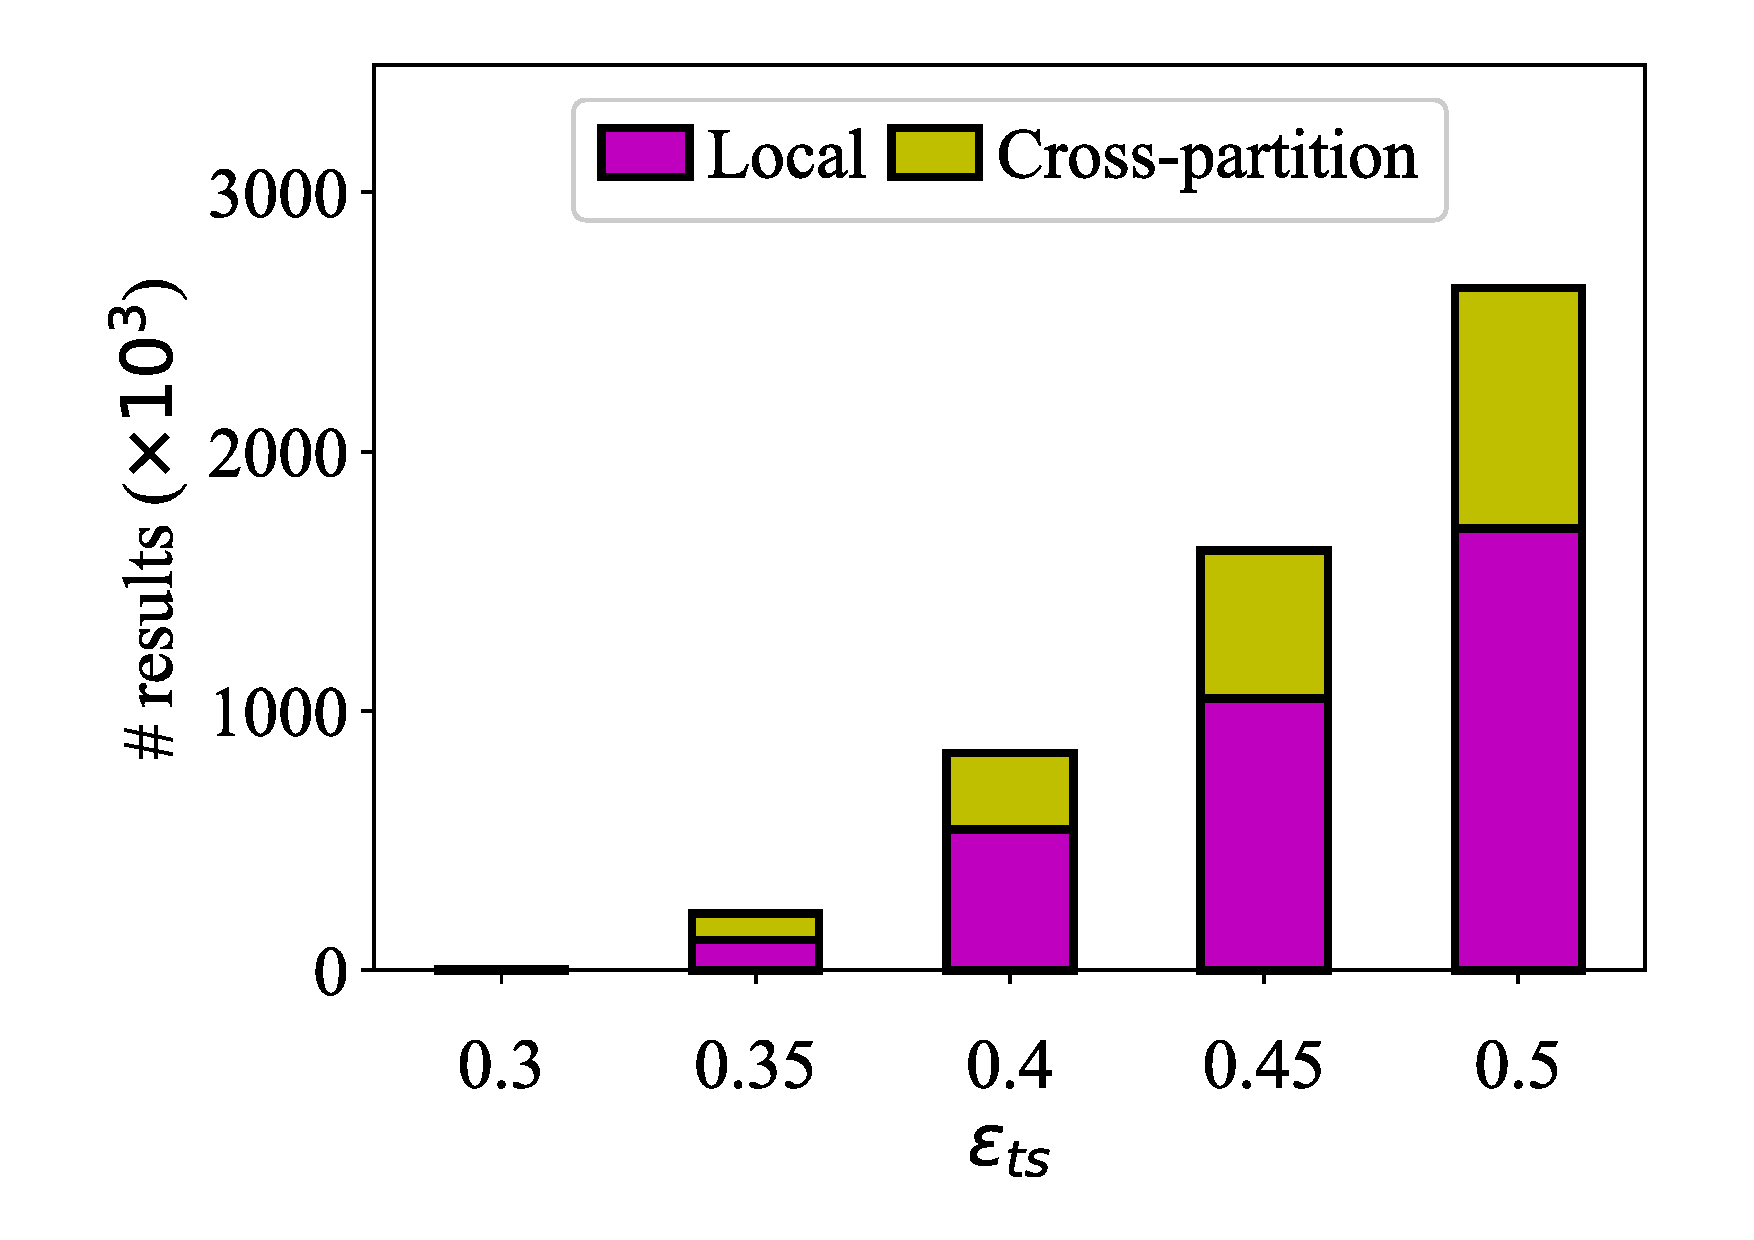
\includegraphics[trim=0 0.5cm 1.4cm 1cm, clip, width=0.325\textwidth]{figures/plots/EpsTSDistResults.pdf}\label{exp:EpsTSDistResults}}
 \caption{Performance results for the {\em distributed} methods with varying $\epsilon_{ts}$.}
 \label{exp:distr_EpsTS}
\end{figure}

Figure \ref{exp:scalability} concerns scalability of the distributed methods with increasing dataset sizes. For smaller datasets, both methods are competitive, but response times for \base escalate with larger sizes. With 2 million geolocated time series as input, this method did not finish, as it required traversal of too many paths in its underlying R-trees per partition, exceeding the capabilities of the workers. Regarding communication (Figure \ref{sexp:ScalabilityCommunication}), \base requires shuffling of more raw data, especially for input size of 1.5 million. In contrast, \opt maintains lower communication overhead, as it uses light-weight indices to guide data shuffling. Figure \ref{exp:ScalabilityResults} indicates that the number of results is growing according to the input size, as the spatial density also increases with larger synthetic datasets that still cover  the same area (Alicante).

 \begin{figure}[!ht]
 \centering 
 \subfloat[Query response time]{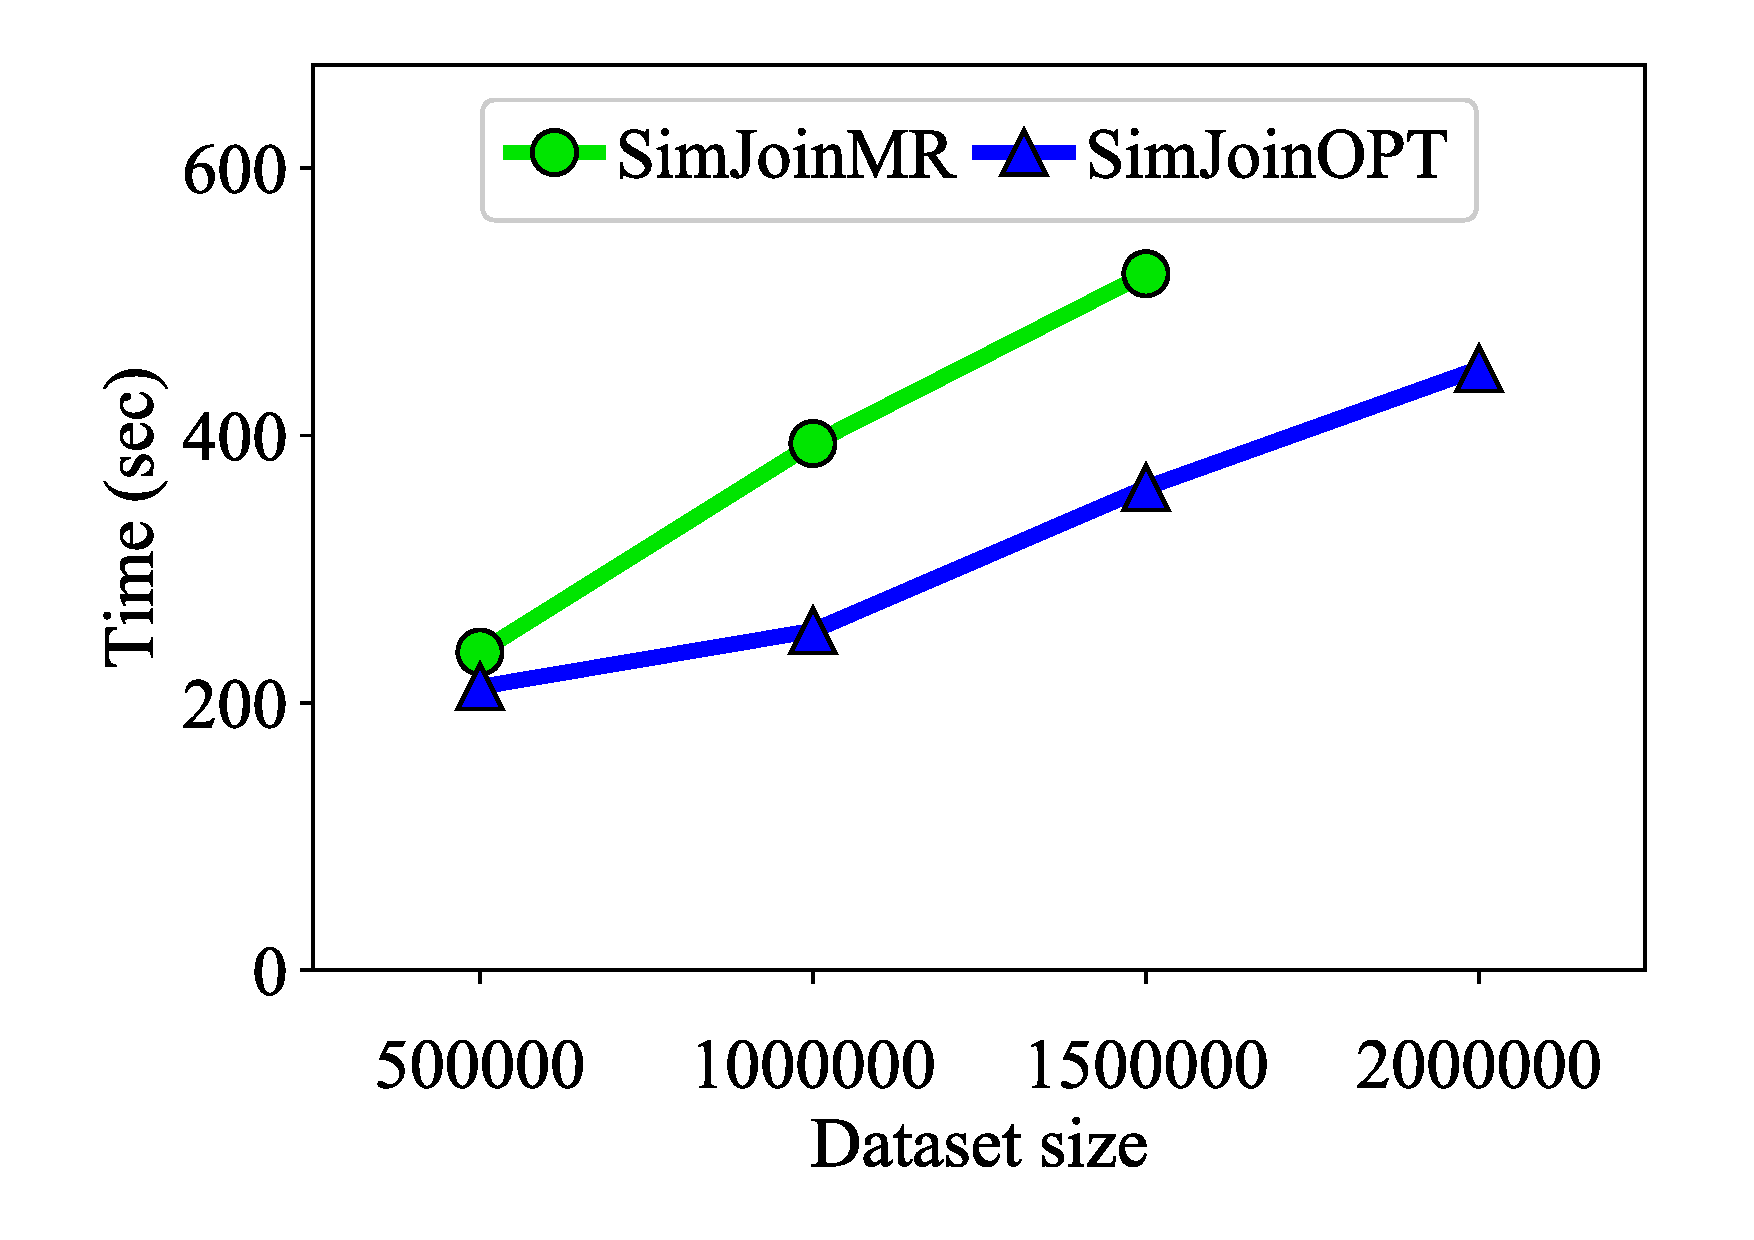
\includegraphics[trim=0.5cm 0.5cm 1cm 1cm, clip, width=0.325\textwidth]{figures/plots/ScalabilityDist.pdf}\label{exp:ScalabilityDist}}
 \subfloat[Geolocated time series shuffled]{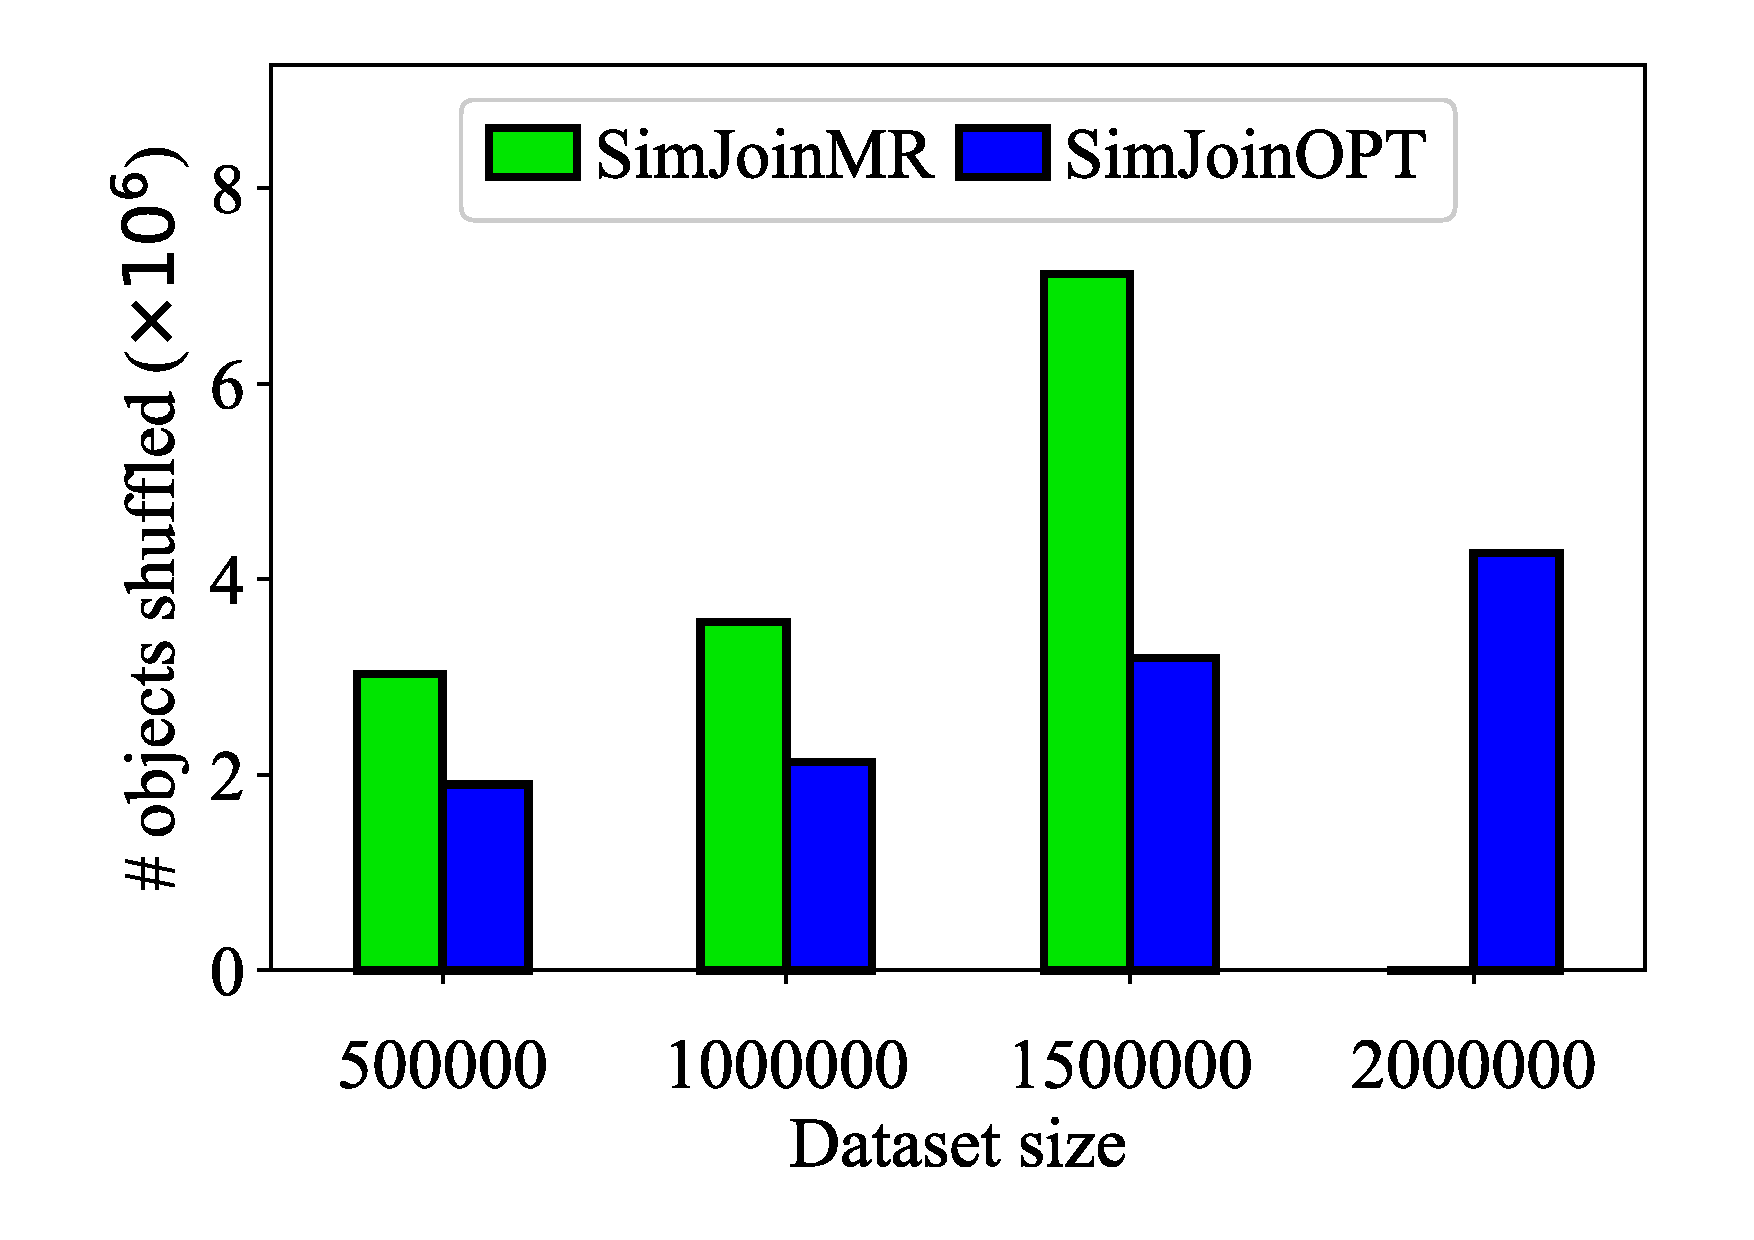
\includegraphics[trim=0.5cm 0.5cm 1cm 1cm, clip, width=0.325\textwidth]{figures/plots/ScalabilityCommunication.pdf}\label{sexp:ScalabilityCommunication}}
 \subfloat[Query results per phase]{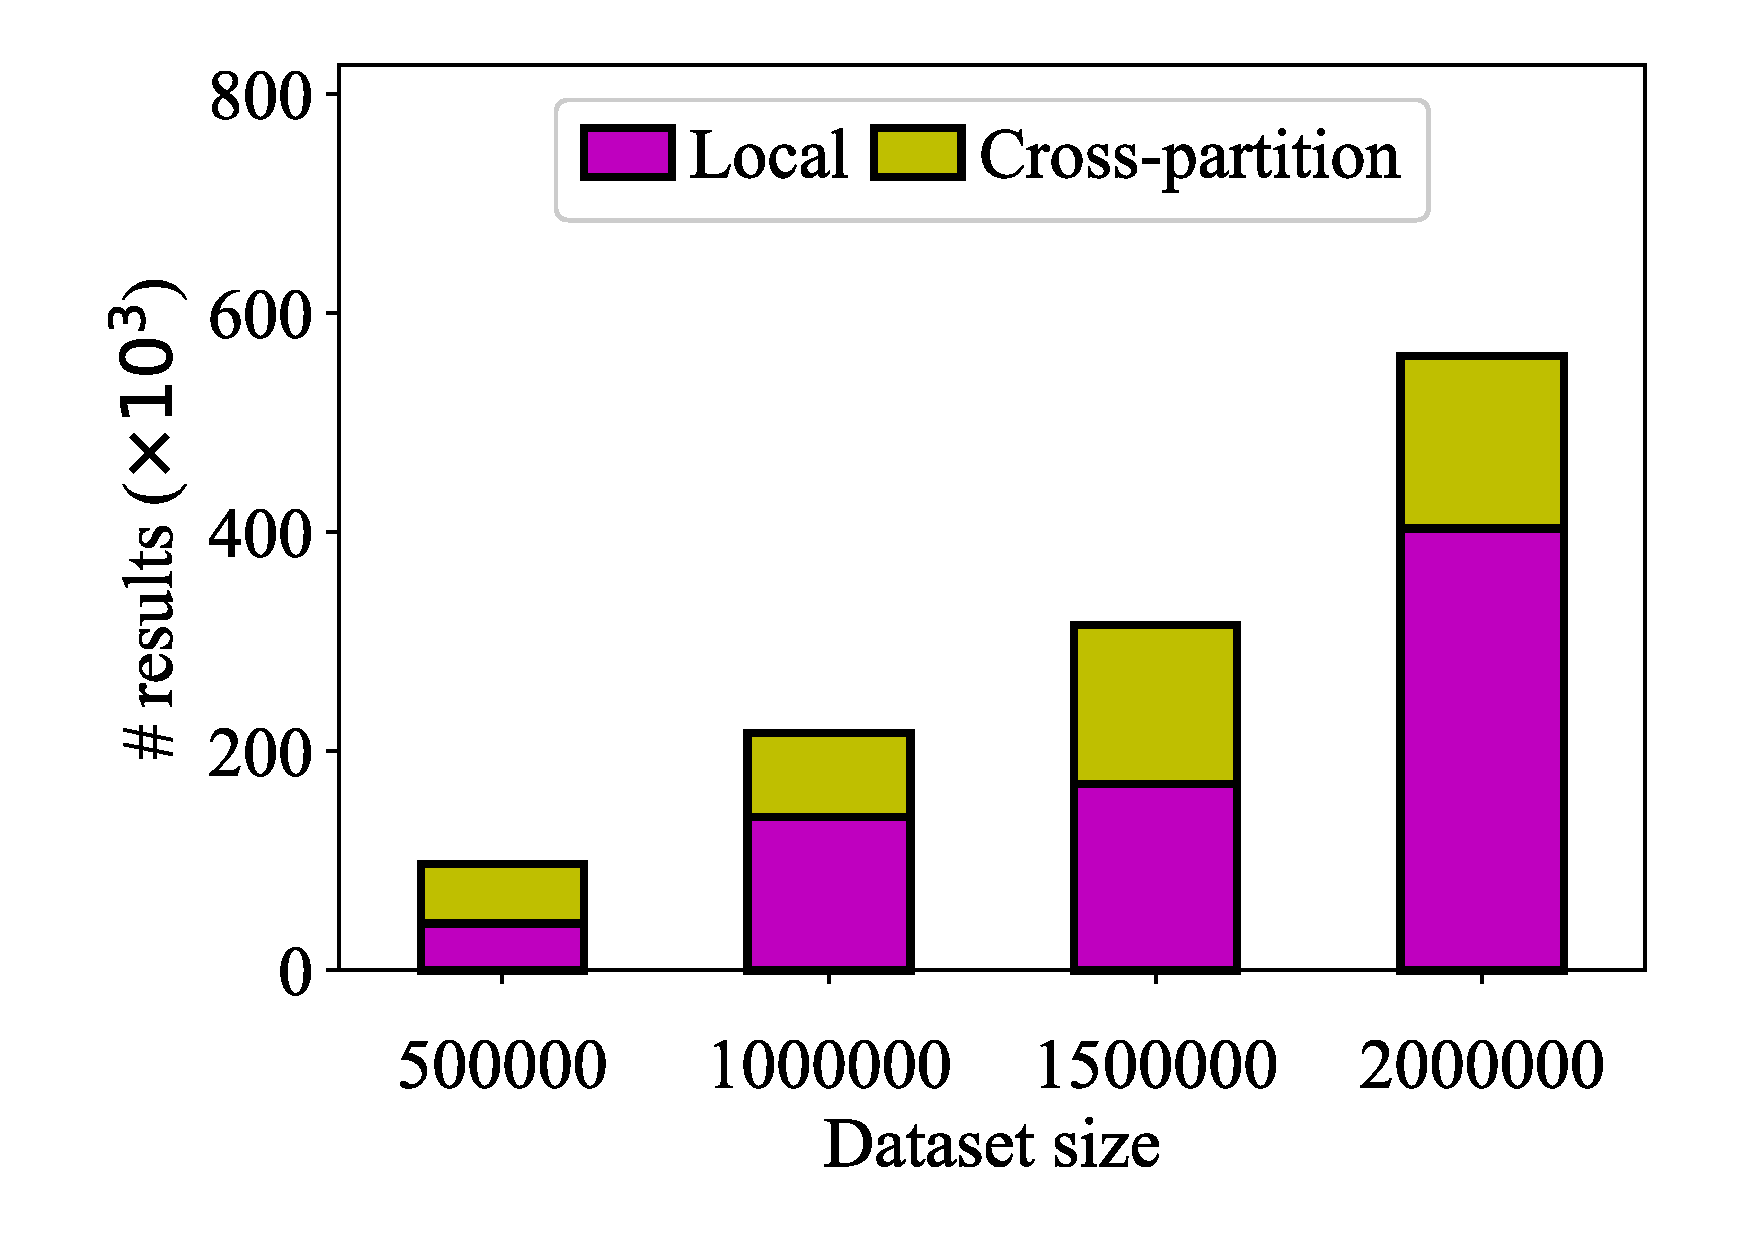
\includegraphics[trim=0.3cm 0.5cm 1.2cm 1cm, clip, width=0.325\textwidth]{figures/plots/ScalabilityResults.pdf}\label{exp:ScalabilityResults}}
 \caption{Scalability of the {\em distributed} methods.}
 \label{exp:scalability}
\end{figure}

Last but not least, we conducted tests concerning partitioning, i.e., varying the grid granularity and distributing input data accordingly. As shown in Figure \ref{exp:Partitioning}, \base was not able to conclude its evaluation over coarser spatial subdivisions, as each resulting partition can hardly cope with the larger subsets of data held locally. For $30 \times 30$ partitions, \opt performs better thanks to  the superiority of \btsr in pruning. But \base overtakes \opt when allowing finer partitioning ($40 \times 40$ partitions or more), as the \rtree overhead diminishes. Each such index has to deal with smaller subsets, although it incurs higher communication overhead compared to \opt (Figure \ref{exp:PartitioningCommunication}). Indeed, having more partitions forces \opt to search for joins pairwise in many more bands and boxes, while also building the respective intermediate indices. So, such optimization really compensates with a coarser partitioning, achieving its best performance with a $20 \times 20$ grid as depicted in Figure \ref{exp:Partitioning}. Finally, Figure \ref{exp:PartitioningResults} indicates that the majority of resulting pairs are derived locally under a coarser partitioning. However, this is reversed with finer partitioning, as the size of blocks (bands and boxes) during the cross-partition checks cover much more area per cell, hence many more qualifying pairs are found while searching across neighboring partitions.


 \begin{figure}[!ht]
 \centering
 \subfloat[Query response time]{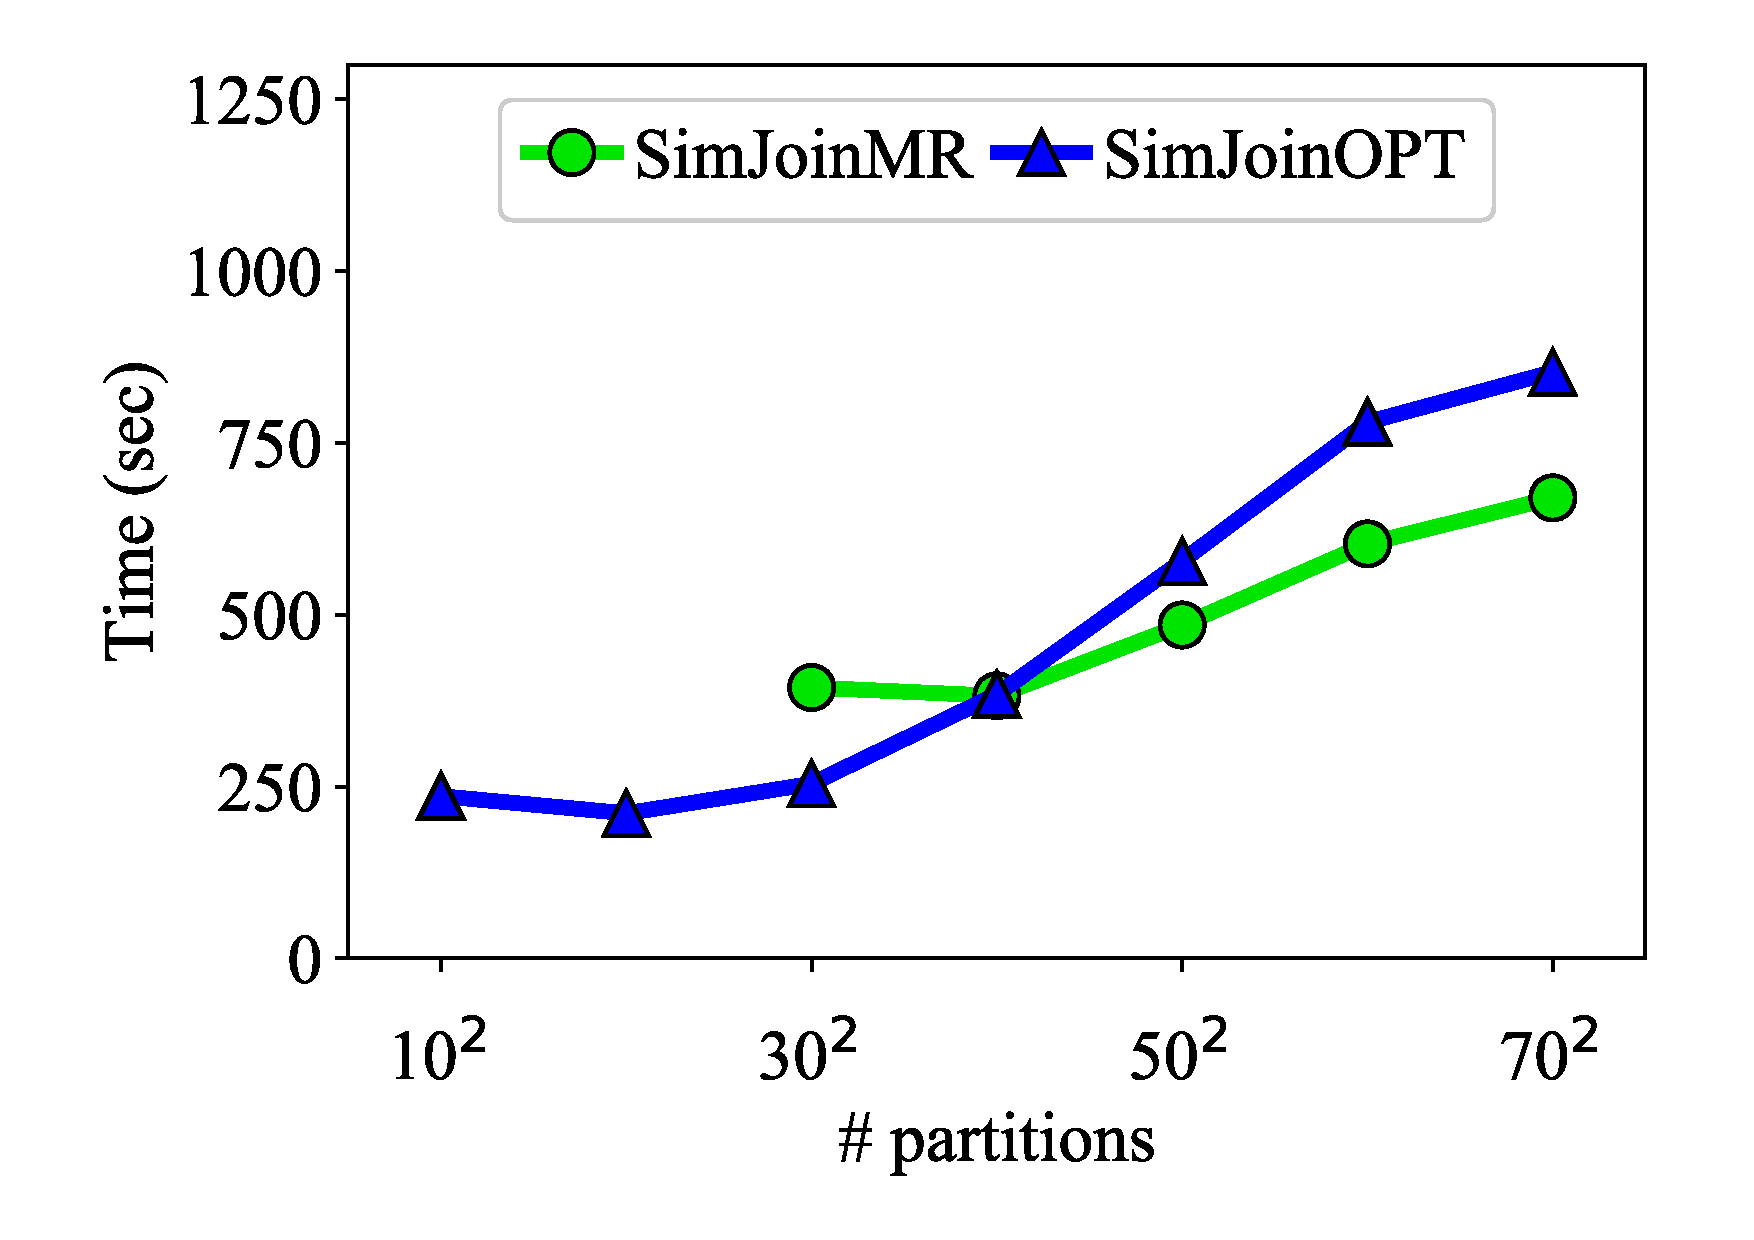
\includegraphics[trim=0.5cm 0.5cm 1cm 1cm, clip, width=0.325\textwidth]{figures/plots/Partitioning.pdf}\label{exp:Partitioning}}
 \subfloat[Geolocated time series shuffled]{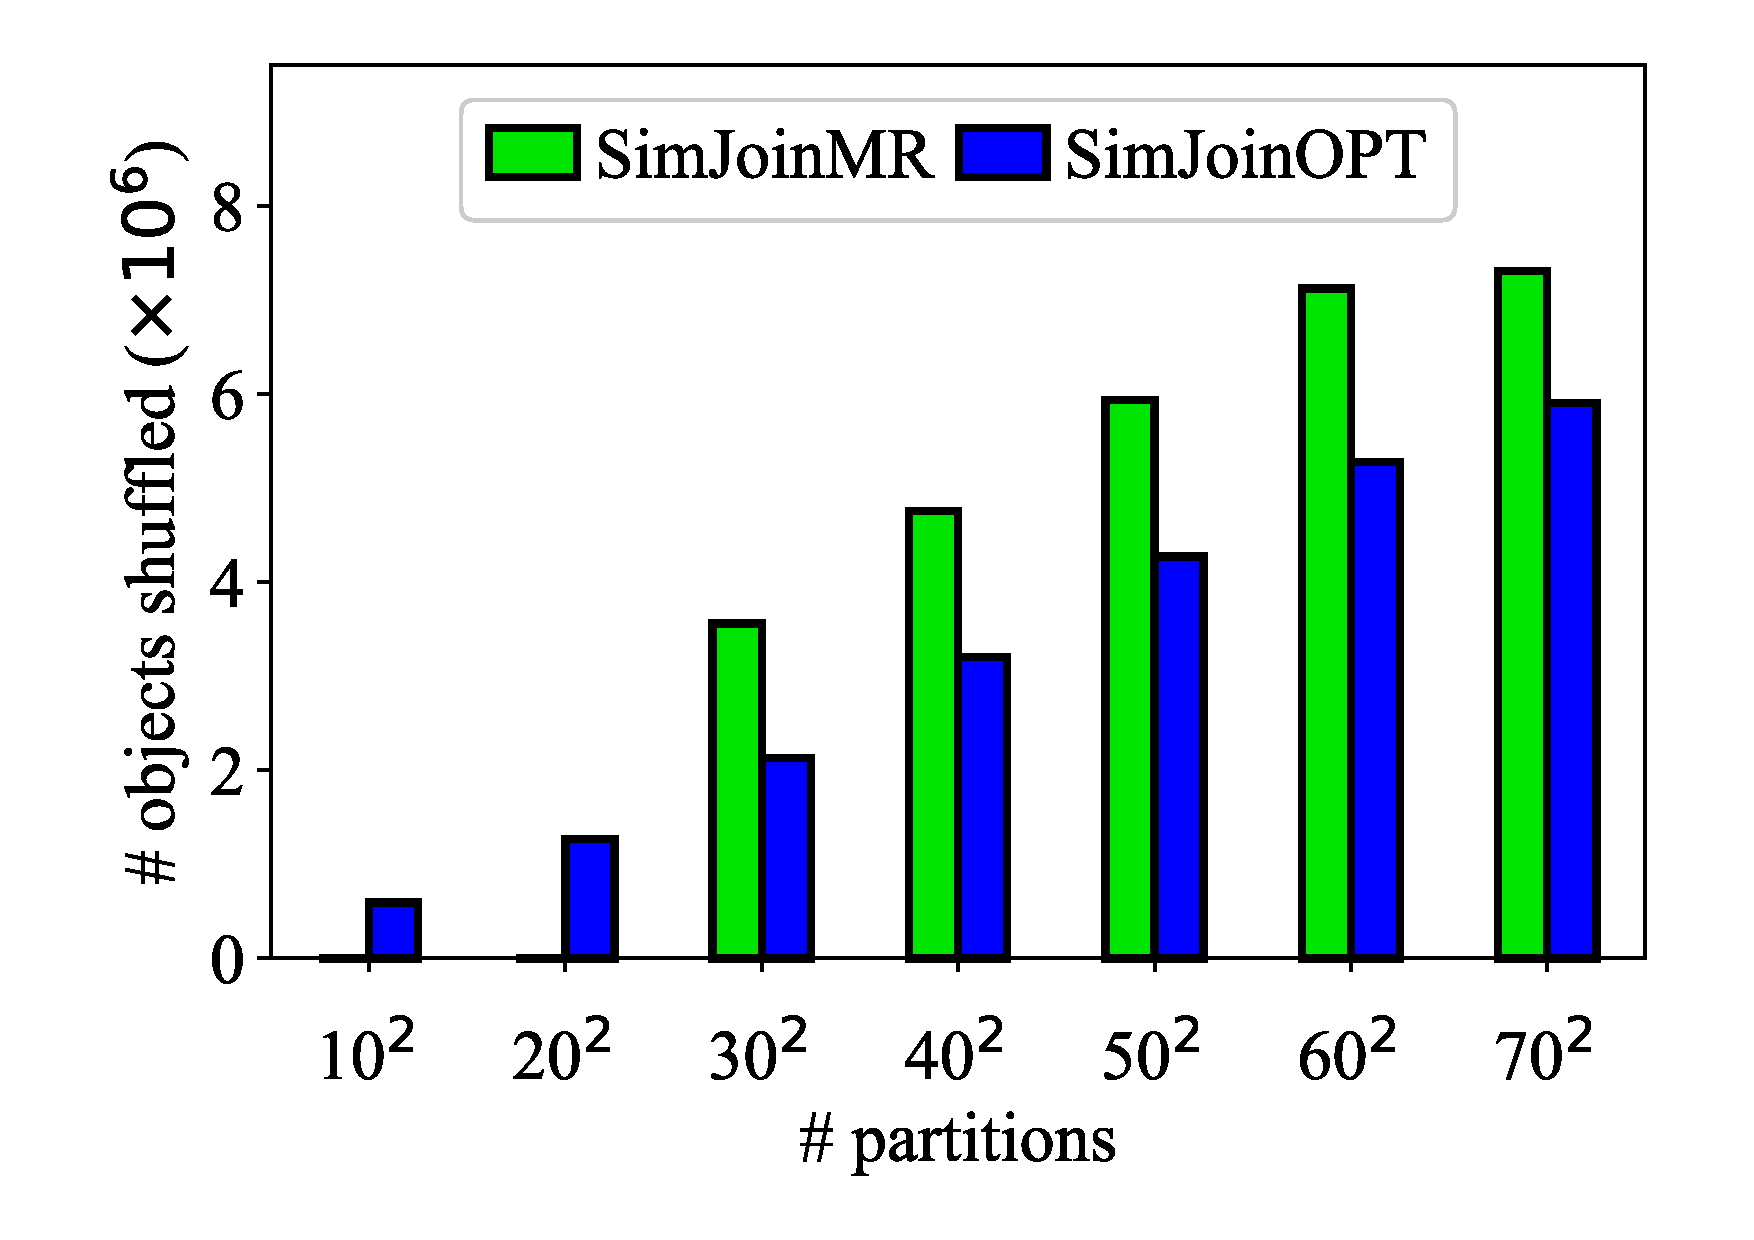
\includegraphics[trim=0.5cm 0.5cm 1cm 1cm, clip, width=0.325\textwidth]{figures/plots/PartitioningCommunication.pdf}\label{exp:PartitioningCommunication}}
 \subfloat[Query results per phase]{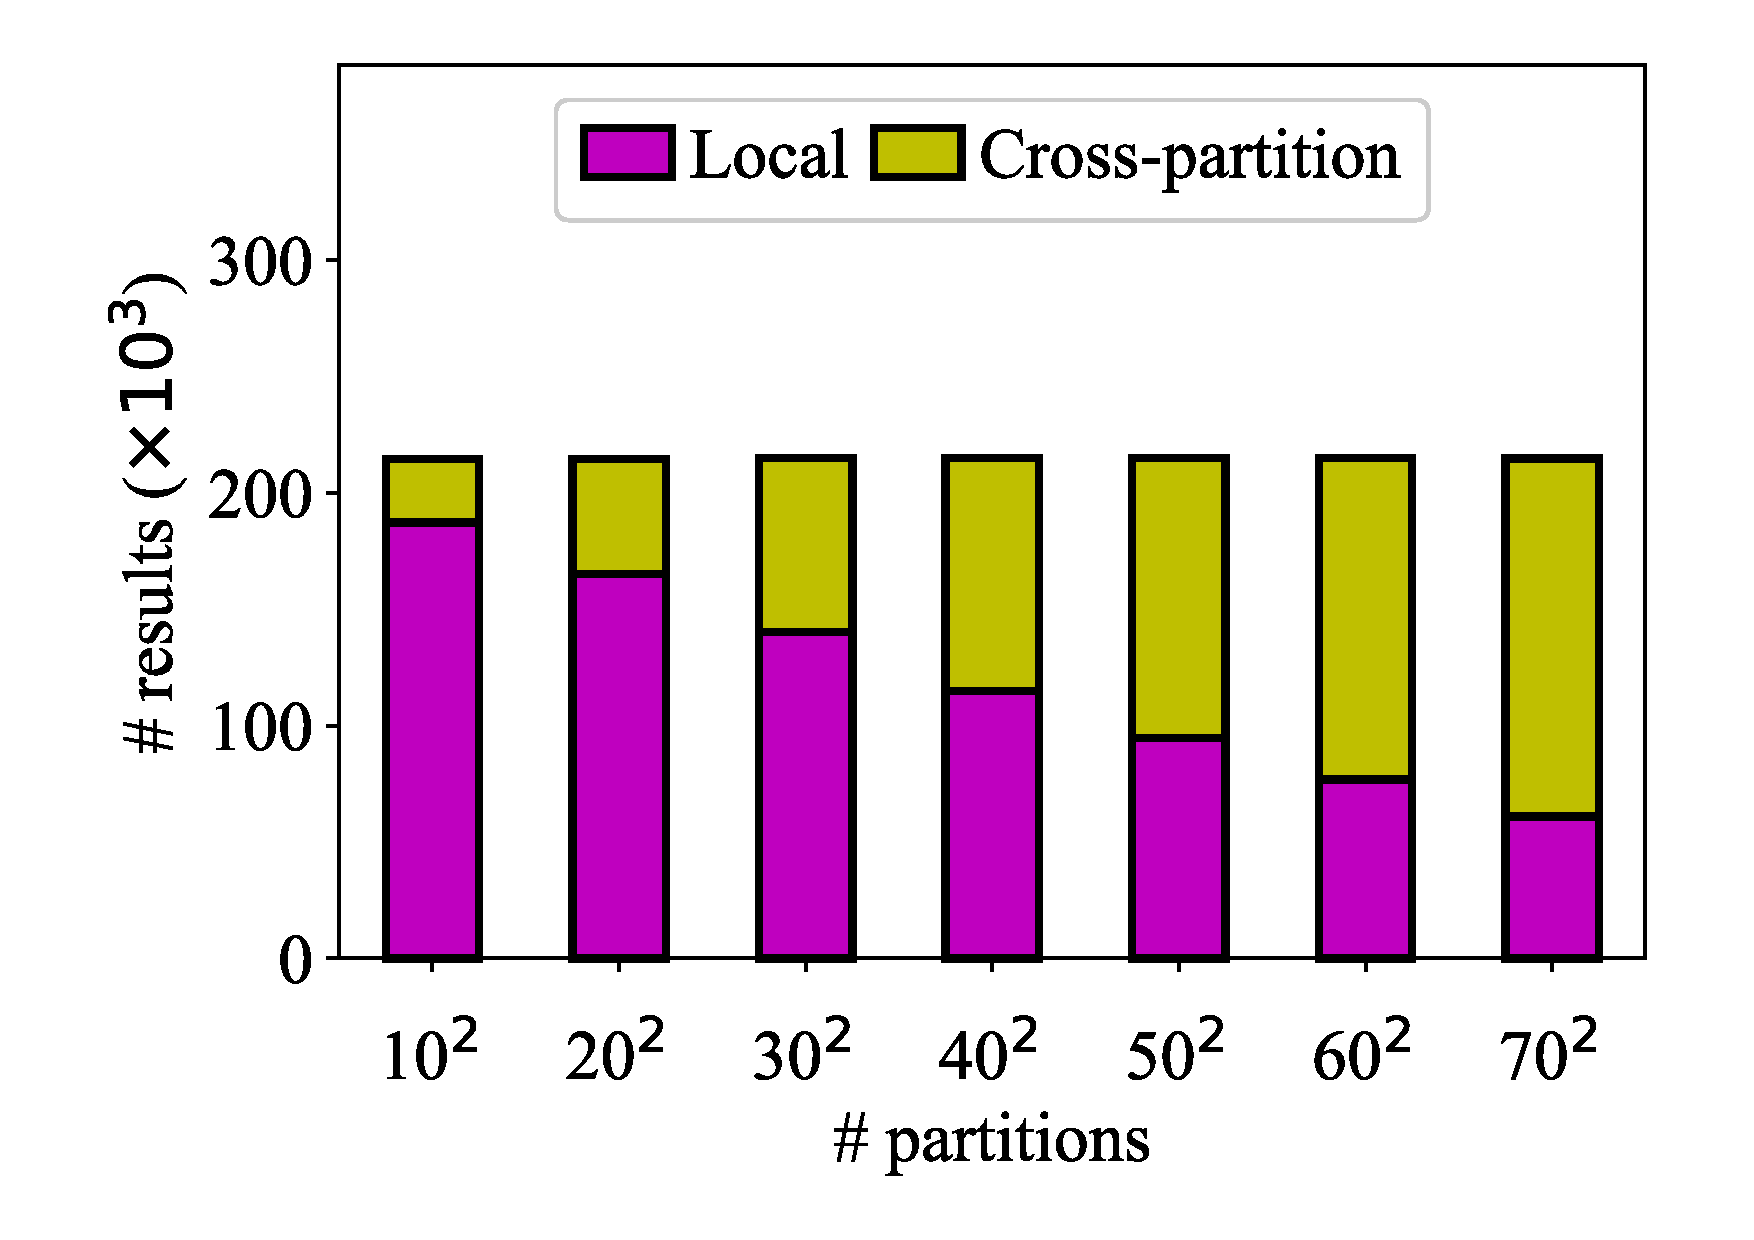
\includegraphics[trim=0.3cm 0.5cm 1.2cm 1cm, clip, width=0.325\textwidth]{figures/plots/PartitioningResults.pdf}\label{exp:PartitioningResults}}
 \caption{Effect of partitioning on the performance of {\em distributed} methods.}
 \label{exp:partitioning}
\end{figure}